\documentclass[a4paper,12pt,openright,twoside]{book}
\usepackage[latin1]{inputenc}
\usepackage{amsmath}
\usepackage{amsfonts}
\usepackage{amssymb}
\usepackage[dvips]{graphicx}
\usepackage{makeidx}
\usepackage{moreverb}
\usepackage{multirow}
\usepackage{parskip}
\usepackage{longtable}
\usepackage{rotating}
\usepackage{array}
\usepackage{listings}
\usepackage[amssymb]{SIunits}
%\usepackage{hyperref}
\usepackage{color}
\usepackage[page,title]{appendix}
\usepackage[onehalfspacing]{setspace}
\newcommand{\mat}{\mathbf}
\usepackage[justification=centering, font=singlespacing]{caption}
% \oddsidemargin 0.72in \evensidemargin 0.12in
%\textwidth 6.15in \topmargin -0.60in \headheight -.0in \textheight 9.210in
\usepackage{vmargin}
\setpapersize{A4}
\setmarginsrb{40mm}{20mm}{20mm}{20mm}
{0pt}{0pt}{12pt}{30pt}
\pagestyle{plain}
%\newenvironment{refs}{
%\begin{list}{}{\leftmargin=0.5cm \topsep=0.06cm \itemindent=-0.5cm
%\listparindent=-0.5cm \parsep=0.035cm
%\itemsep=0.0cm}\item[]}{\end{list}}

%floats
%\renewcommand\floatpagefraction{.9}
%\renewcommand\topfraction{.9}
%\renewcommand\bottomfraction{.9}
%\renewcommand\textfraction{.1}   
%\setcounter{totalnumber}{50}
%\setcounter{topnumber}{50}
%\setcounter{bottomnumber}{50}

%\includeonly{Introduction}

\begin{document}
\begin{titlepage}
\vspace*{\fill}
\begin{center}
{\huge Derivation and Analysis of Malaria Parasite Clearance Times}\\[1cm]
by\\[1cm]
{\large Nicholas Robert George Shrine}\\[4cm]
Submitted in partial fulfilment of the requirements for the MSc in Statistics\\
Department of Probability \& Statistics\\[2cm]
September 2009
\end{center}
\vspace*{\fill}
\end{titlepage}
\clearpage{\pagestyle{empty}\cleardoublepage}
\frontmatter
Abstract of: Derivation and Analysis of Malaria Parasite Clearance Times\\[0.5cm]
Author: Nicholas Robert George Shrine\\[0.5cm]
Date: September 2009\\[0.1cm]
\setlength{\parindent}{0.4in}
\setlength{\parskip}{0.0in}

A clinical trial by Glaxo Smithkline was performed to compare the parasite clearance times for an antimalarial drug used alone and in combination with another drug. The primary endpoint is the time at which 90\% of the parasites have been cleared from the blood (PC90). The data consists of parasite counts per microlitre of blood before first dose of antimalarial and then at multiple times up to 48 hours from first dose for each of 43 subjects. There were 22 male and 21 female subjects, with 23 on the single-drug treatment and 20 on the combined-drug. Subjects were treated at two centres, with 24 and 19 at each respectively. 

Three methods were investigated for making interpolated estimates of the PC90 time between times at which parasite counts were taken: linear cubic polynomial regression, non-linear logistic regression and simple log-linear interpolation. The log-linear interpolation method was identified as the most suitable with problems with logistic regression previously applied to this data highlighted.

The estimated PC90 clearance times were analysed by 3-way ANOVA by centre, sex and treatment using appropriate variance stabilising transformations. There is evidence to reject the hypothesis of no interaction of sex and treatment ($p<0.05$). It is found that female subjects on the combined treatment have mean PC90 13.1 hours shorter (95\% confidence interval: 5.0, 22.7 hours) than on the single-drug treatment. There is no evidence to reject the hypothesis at the 5\% level that male subjects have the same mean PC90 on both treatments. The results of non-parametric resampling tests confirm the conclusions of the parametric analysis.

No evidence of a difference in mean PC50 between groups was found at the 5\% level. Good evidence to reject the hypothesis of mean PC99 times being equal between treatment groups was found ($p<0.0005$), with mean PC99 times for subjects on the combined-drug treatment being 12 hours shorter (95\% CI: 8, 16) than for subjects on the single drug.

The decrease in clearance times for combined-drug therapy is observed in other similar studies, but no other study reviewed finds a sex-treatment interaction effect.

Functional data analysis, used to model the speed of clearance, finds that the combined-drug treatment reaches its maximum rate of clearance 15 hours before the single-drug treatment.
\pagebreak
\begin{center}
{\large Acknowledgements}\\[1cm]
\end{center}
The author acknowledges Glaxo Smithkline for the provision of the data analysed in this dissertation.
%I would also like to thank my dissertation supervisor Professor John Biggins and all the members of staff involved with the MSc course at Sheffield. 

\pagebreak
\vspace*{\fill}
{\large The views and opinion contained in this dissertation shall not be construed or interpreted whether directly or indirectly to be the views or opinions of any of the officers or employees of GlaxoSmithKline Research and Development Limited or any of its affiliated companies forming part of the GlaxoSmithKline group of companies. Further, reliance on the information contained in this dissertation is at sole risk of the user. The information is provided ``as is" without any warranty or implied term of any kind, either express or implied, including but not limited to any implied warranties or implied terms as to quality, fitness for a particular purpose or non infringement. All such implied terms and warranties are hereby excluded.}
\vspace*{\fill}
\tableofcontents
%\listoffigures 

\mainmatter
\setlength{\parindent}{0.0in}
\setlength{\parskip}{0.1in}
\chapter{Introduction}\label{ch:intro}
\section{Background}
\subsection{Malaria}
Malaria is a serious, potentially fatal disease caused by infection of the blood by a parasitic organism. The parasite is transmitted between people by mosquito bites. Over one million people a year die of malaria and this number is rising due to increasing resistance of the parasite to antimalarial drugs\cite{who}. Malaria is also a health hazard for people travelling to areas of the world where Malaria is endemic.

Treatment for malaria is by drug therapy, often using a combination of drugs. Unlike many other diseases the level of infection in cases of malaria may be quantified by counting the number of parasites present\cite{white}. Therefore, a measure of the efficacy of an antimalarial drug treatment is the reduction in the number of parasites in the blood. 

\subsection{Clinical trials for antimalarial drug treatments}
The World Health Organization (WHO) uses systematic reviews of randomized trials, that compare two or more treatments, as its basis for recommendation of malaria treatment\cite{who}. Many recent studies are now looking at how to treat drug-resistant malaria with combined-drug treatments, primarily in areas of the world where there is a high prevalence of drug-resistant strains of the parasite such as south-east Asia\cite{smithuis}. Based on systematic review of randomized clinical trials, the The WHO recommends Artesiminin\footnote{Artesiminin is a drug that has been used in China for thousands of years \texttt{http://en.wikipedia.org/wiki/Artemisinin}}-based combination therapy over other combination therapies or single-drug treatments\cite{who}. 

\subsubsection*{Protocols}
A common technique is a randomized, double-blind trial are used where the randomization is performed by computer code\cite{bell, newton, vries}. Open label studies are also used\cite{wootton, smithuis}, perhaps with partial blinding, for example when the subjects and clinicians know which treatment is being administered, but the technicians analysing the data do not\cite{wootton}. Non-randomized studies are also used whereby patients are allocated to treatments based on symptoms and level of infection\cite{carmello}.

\subsubsection*{Data collection}
Generally the parasite count per microlitre are obtained my taking blood samples from subjects at multiple times after treatment and counting the parasites present by microscopy. The WHO recommends that all blood samples should be checked by two microscopists and that the average of the two counts be used\cite{protocolWHO}.

\subsubsection*{Endpoints}
In comparing malaria treatments various endpoints are used. One of the most common ones in the parasite clearance time (PCT), usually the time until parasites are no longer detectable on a blood film\cite{white}. Other commonly used times are PC50, PC90 and PC99 which are the time for 50\%, 90\% and 99\% of the parasites to be cleared from the blood respectively. These times are determined by comparing the parasite count before treatment (the \textit{baseline}) with the count taken at time intervals after first treatment. As the parasite count will usually fall to one of the endpoint percentages between counts being taken some method of interpolation is required to infer the time to the chosen endpoint.

Another endpoint used is the parasite reduction ratio (PRR), which is the reduction in the parasite count over a certain time period. White\cite{white} states that the parasite reduction ratio over 48 hours (PRR$_{48}$) is a useful index as 48 hours is the asexual lifecycle of the parasite. Carmello \textit{et al.}\cite{carmello} also use the parasite reduction rate at 24 hours (PRR$_{24}$) and the percentage of patients with no detectable parasites after 48 hours (PPUP$_{48}$).

Sometimes symptomatic endpoints are used rather than parasite reduction levels.  Fever clearance times, the time for the axillary temperature to fall below 37.5$^\circ$C, is one such measure\cite{bell,newton}.

\subsubsection*{Statistical methodology}
The parasite count is usually analysed after logarithmic transformation\cite{wootton, vries, carmello}, although no explicit justification for this is given in the literature reviewed here. Times to reduce the parasite count by 50\%, 90\% and 99\% (PC$_{50}$, PC$_{90}$ and PC$_{99}$) are calculated by interpolating between parasite counts at times straddling the time of interest, either by a linear (actually log-linear) interpolation\cite{carmello, newton} or the fitting of regression mode to the data such as a linear polynomial\cite{vries} or an exponential\cite{vries} or logistic non-linear model\cite{wootton}.

Comparison of parasite clearance times is usually performed using parametric test such as $t$ test and ANOVA stratified by experimental factors\cite{vries, smithuis, wootton, carmello}. Explicit verification of normality, as required by these tests, is not found in the literature. However, some studies make use of equivalent non-parametric tests, for data they identify as non-normal, such as Mann-Whitney, Wilcoxon signed rank test\cite{carmello, newton} and Kruskall-Wallis\cite{pukri}.\label{stat-tests}

For categorical data, such as proportions of patients with no detectable parasites, $\chi^{2}$ tests with Yates' correction and Fisher's exact test are used in some studies\cite{newton, smithuis}.

A 5\% significance level is invariably used, sometimes with a Bonferonni correction for multiple comparisons. 95\% confidence intervals are given as recommended by WHO protocol\cite{protocolWHO}. Some studies include a power calculation such as Wootton \textit{et. al}\cite{wootton} who calculate that 22 patients are required in each arm to detect a 9 hour change in clearance time with 5\% significance and 90\% power; Newton \textit{et al.}\cite{newton} give power calculations for mortality rates.
\section{The Glaxo Smithkline Clinical Trial}
A clinical trial was conducted by Glaxo Smithkline (GSK) comparing parasite clearance times for an existing antimalarial drug against those for this drug when administered in combination with different dose levels of another antimalarial. Parasite counts per microlitre were recorded from blood samples taken prior to first dose (baseline) and then at multiple time points (1, 2, 3, 4, 6, 8, 12, 18, 24, 30, 36, 42, 48 hours) after first dose.

\subsection{Data description}
The data were received as an email attachment from our contact at Glaxo Smithkline. The attachment was a \emph{SAS} data set which was able to be read into \emph{R} by first exporting from \emph{SAS} in dbf format and then read into \emph{R} using the \texttt{read.dbf} function.
Table \ref{rdata} shows the data as an \emph{R} data frame. 
\begin{table}[h]
\centering
\caption{Data as an R data frame}\label{rdata}
\begin{boxedverbatim}
CENTREID SUBJID SEX                    plantm   acttm  parct trt
     001     54   M                  PRE-DOSE -2.8333  14092   A  
     001     54   M  2 HOURS AFTER FIRST DOSE  2.0333   7592   A  
     001     54   M  4 HOURS AFTER FIRST DOSE  4.0500   1170   A  
     001     54   M  6 HOURS AFTER FIRST DOSE  6.0000     52   A  
     001     54   M  8 HOURS AFTER FIRST DOSE  8.0500      0   A  
\end{boxedverbatim}
\end{table}

The columns are:
\begin{itemize}
\item\texttt{CENTREID} - The centre at which the study was undertaken, either centre \texttt{001} or \texttt{002}.
\item\texttt{SUBJID} - A numerical identifier for each subject (patient) participating in the trial. There are 43 subjects.
\item\texttt{SEX} - The sex of each subject, either \texttt{M} for male or \texttt{F} for female.
\item\texttt{plantm} - The planned time of taking a blood sample for measuring parasite load, either \texttt{PRE-DOSE} i.e. before the drug treatment is administered, or \texttt{n HOURS AFTER FIRST DOSE}.
\item\texttt{acttm} - The actual time in hours that the blood sample was taken relative to the time the treatment was administered, hence all pre-dose times are negative.
\item\texttt{parct} - The parasite count per $\mu L$ of blood.
\item\texttt{trt} - An indicator of which treatment was used \texttt{A} or \texttt{B}.
\item\texttt{trttxt} (not shown) - A description of treatments \texttt{A} and \texttt{B}: \texttt{alone}, meaning that a single drug was used or \texttt{combi} meaning that a combination treatment was used.
\end{itemize}

As this data was released by GSK purely for training purposes only the minimum data was disclosed to allow a methodological study of estimating and analysing parasite clearance times. Hence, we have no information on the actual drug combination used, nor the dosage. We know nothing more about the subject than their sex, nor how they were allocated to treatment groups.

\section{Project Aims}
\subsection{Derivation of parasite clearance times}
It was stated by GSK that the endpoint of primary importance in this trial was PC90 i.e. the time for the parasite count to be reduced 90\% from its baseline ``PRE-DOSE'' level. Accordingly, one of the aims of this project is to investigate methods for estimating the time to PC90 with a view to the method being able to be applied to large number of patients in a clinical trial setting automatically i.e. giving an estimate from the data via a computer function without human input being required for every estimate.

It was stated by our contact at GSK that an approach based on logistic regression had already been used for PC90 estimation on this data. A logistic curve was fitted to the log-transformed parasite counts ($y$) over time. The simple logistic curve used has the following form: 
$$
y=\alpha+\frac{\lambda}{1+e^{-\beta(x-\mu)}}
$$
where $\alpha$ is the lower asymptote, $\alpha+\lambda$ is the upper asymptote, $\mu$ is the time of maximum rate of reduction (i.e. point of inflexion) and $x$ is time from first dose (in hours), $\beta$ is the fitted coefficient for time; $y = log(1 + P_{(time=x)})$ (P is parasite count), hence $P = e^{y}-1$. They stated that model fit and so consequent validity of derived PC90 estimates were then reviewed.

In this study this method based on logistic regression is evaluated and compared to other methods chosen by investigating the form of the parasite count with time from first dose and behaviour around the PC90 region of interest. The aim is to determine the most accurate, precise and practical method of determining the time to PC90 in terms of being implemented in software for automatic PC90 estimation given such data.

\subsection{Analysis of parasite clearance times}
The PC90 parasite clearance times will then be analysed in order to determine the level of evidence that use of the combined drug treatment speeds up eradication of malaria parasites from the blood and, if so, estimate the average decrease in clearance times with the appropriate confidence intervals.

In order to determine the effect of the factors centre, sex and treatment on the clearance time, the appropriate statistical test must be chosen after checking the form of the distribution of the data. This may be parametric tests such as ANOVA or non-parametric; some of the common ones by researchers for this kind of data were summarised on page \pageref{stat-tests}.

\section{Dissertation overview}
\begin{description}
\item[Chapter \ref{ch:intro}, Introduction] - An overview of clinical trials for antimalarial drug treatments is given with a summary of the statistical techniques used in the literature for the kind of parasite count data that is analysed in this dissertation. A description of the data received from GSK is given. The two main aims of this study are outlined.
\item[Chapter \ref{ch:data}, Exploratory data analysis] - Exploratory data analysis of the raw parasite counts is presented. This is initially performed by graphical analysis of the parasite count plotted against time in separate plots for each subject, grouped by centre, sex and treatment. The main features of the data are described and their possible implications for modelling.

The derivation of the parasite count and its distributional properties are discussed. The distribution of the pre-dose count is analysed and a normalizing transformation is suggested.

The development of the parasite count with time is explored graphically by comparing the mean counts between treatments and with some preliminary ANOVA analysis.
\item[Chapter \ref{ch:derivation}, Derivation of clearance times] - An transformation of the count appropriate for clearance time estimation is identified and 3 different methods of estimating the PC90 clearance time are presented based on regression and interpolation techniques.

The performance of the 3 methods is evaluated and compared for consistency or otherwise, both graphically and by statistical tests. The effect on PC90 estimates of interaction between the estimation method and experimental factors is investigated.

The merits of each method are summarized and a recommendation for PC90 estimation is made.
\item[Chapter \ref{ch:analysis}, Analysis of clearance times] - The effect of centre, sex and treatment on PC90 clearance times is investigated graphically.

The residuals from 3-way ANOVA analysis of the clearance times are investigated to determine the distributional properties of clearance times between the groups. Accordingly, a transformation and modelling method are identified in order to make a valid statistical comparison of the treatment effect.

The effect of the treatment and sex and centre factors are quantified with appropriate confidence intervals.
\item[Chapter \ref{ch:alternative}, Alternative measures of clearance times] - Other commonly used clearance times PC50 and PC99 are analysed to complement the analysis in chapter \ref{ch:analysis}.

The relatively new statistical technique of \emph{functional data analysis} is employed to develop a functional model of the parasite clearance profiles for the sex and treatment groups. The effect of treatment on the speed of parasite reduction over time is also investigated using functional data analysis. 
 
\item[Chapter \ref{ch:discussion}] - 

\end{description}

\chapter{Exploratory Data Analysis}\label{ch:data}

\section{Raw count profiles}
Figures \ref{raw1} and \ref{raw2} show the parasite counts plotted against time in hours. The data is as received from GSK. The number above each plot is the patient identifier. Note that the vertical scales vary for each plot in order to show the main features of the data and hence the parasite counts are not directly comparable.
%\begin{figure}[h]
%\centering
%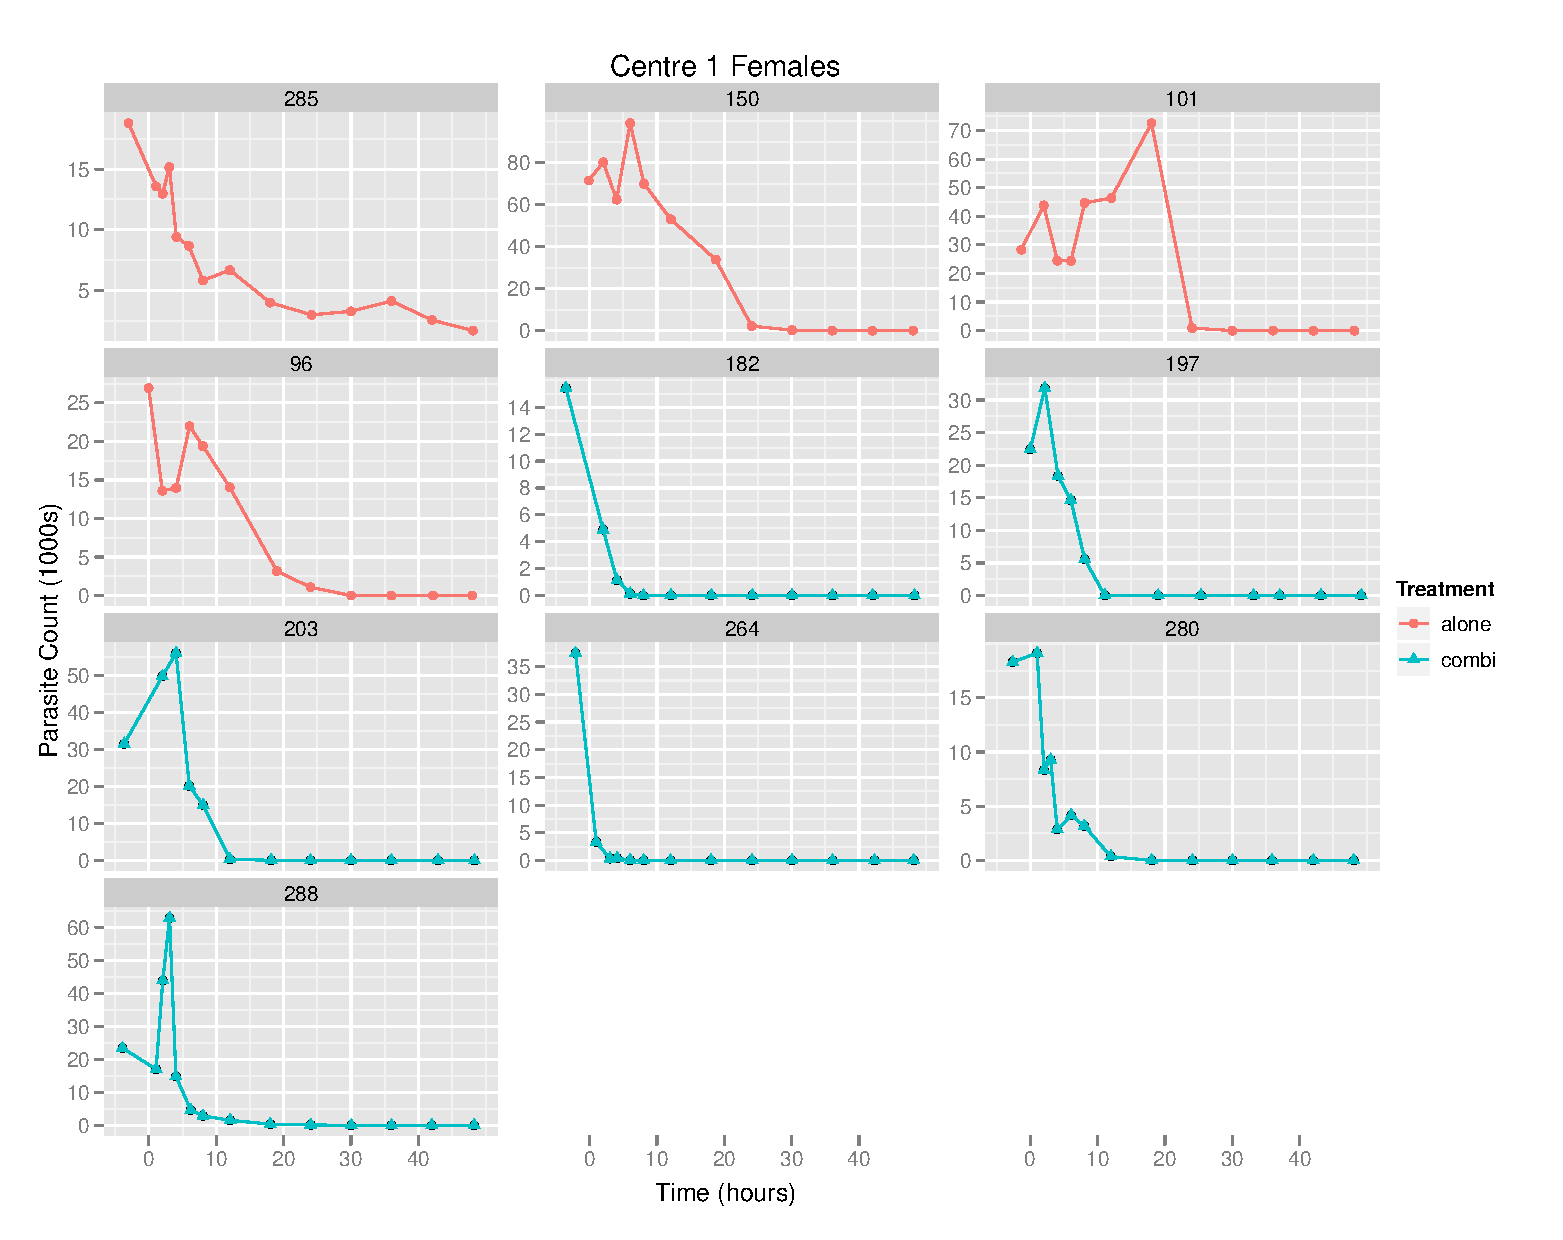
\includegraphics[width=150mm]{raw1f.eps}
%\caption{Parasite count for centre 1 females}\label{raw1F}
%\end{figure} 
%\begin{figure}[h]
%\centering
%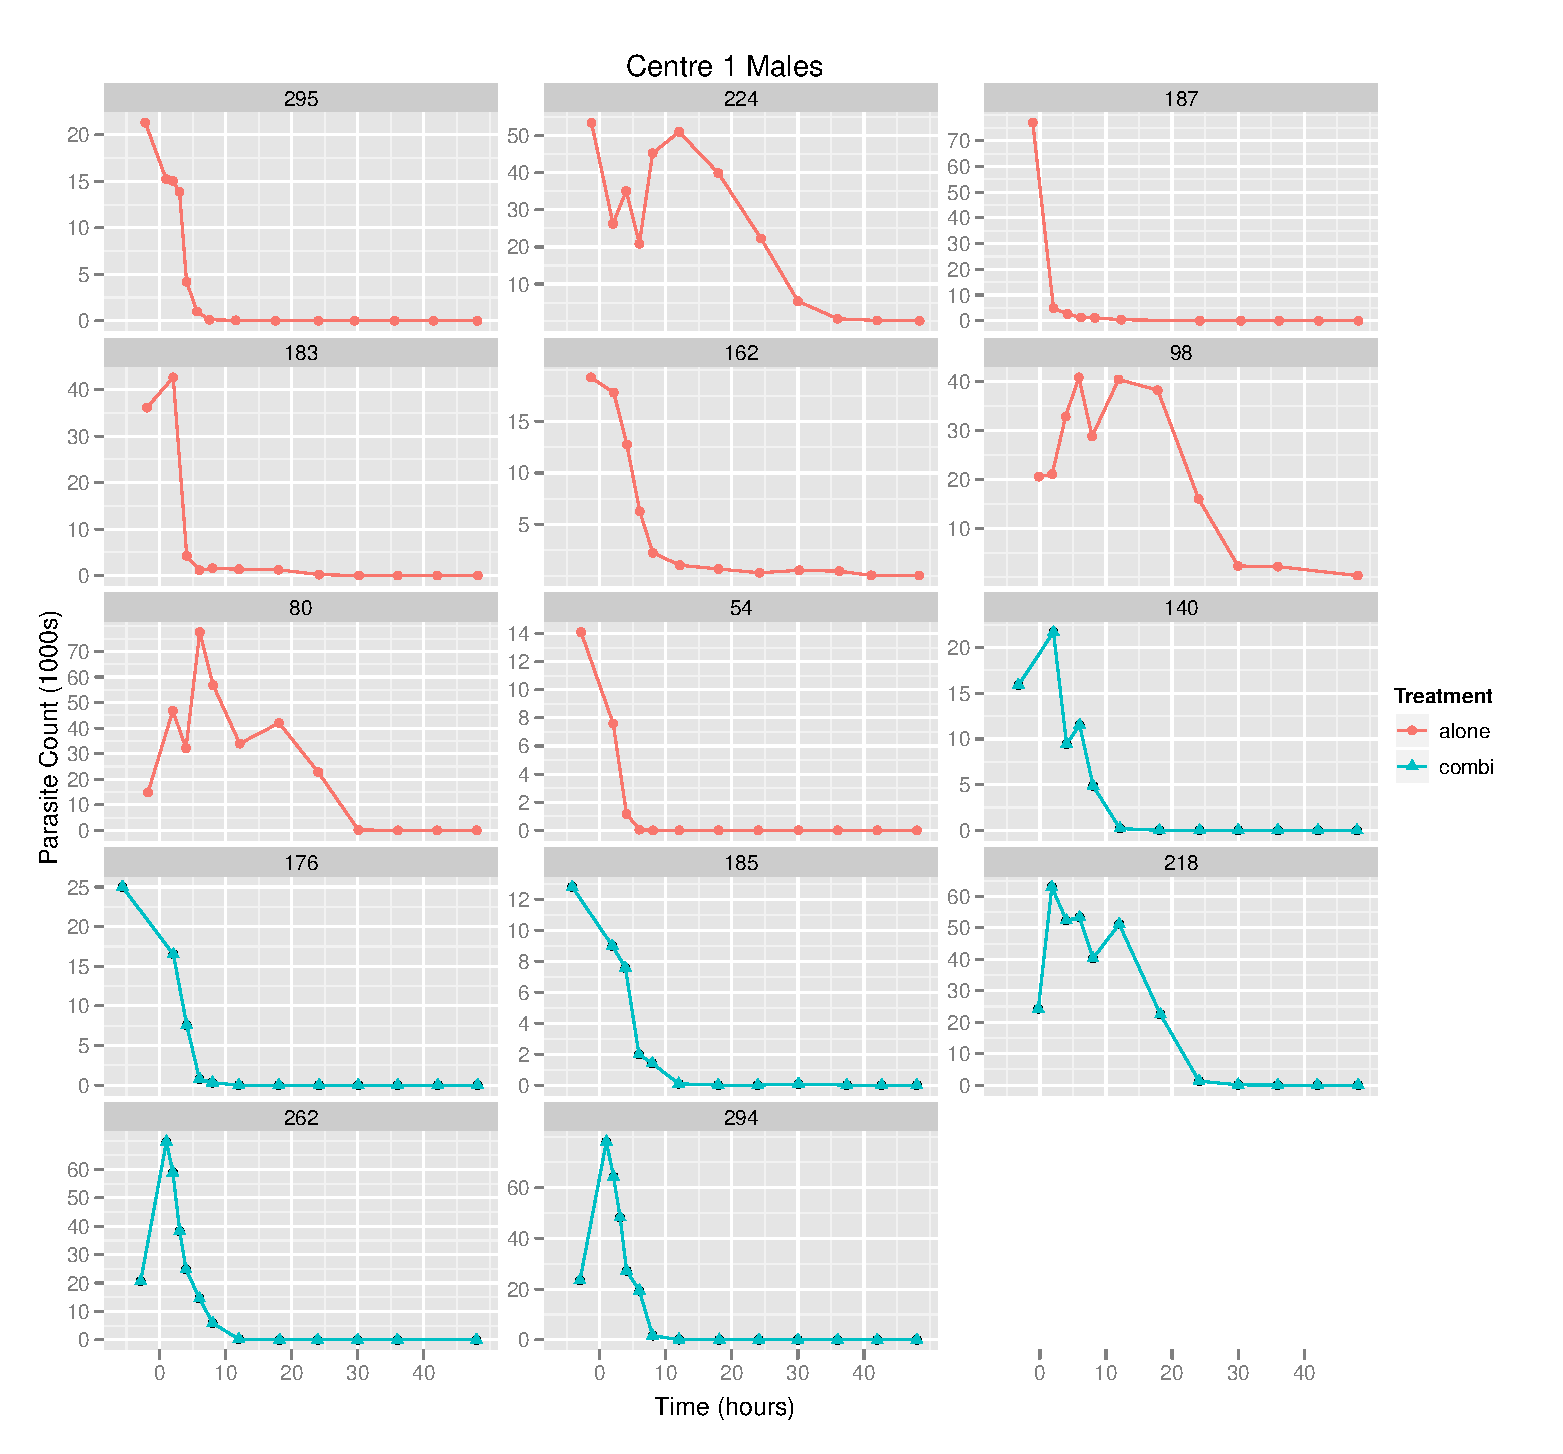
\includegraphics[width=150mm]{raw1m.eps}
%\caption{Parasite count for centre 1 males}\label{raw1M}
%\end{figure} 
%\begin{figure}[h]
%\centering
%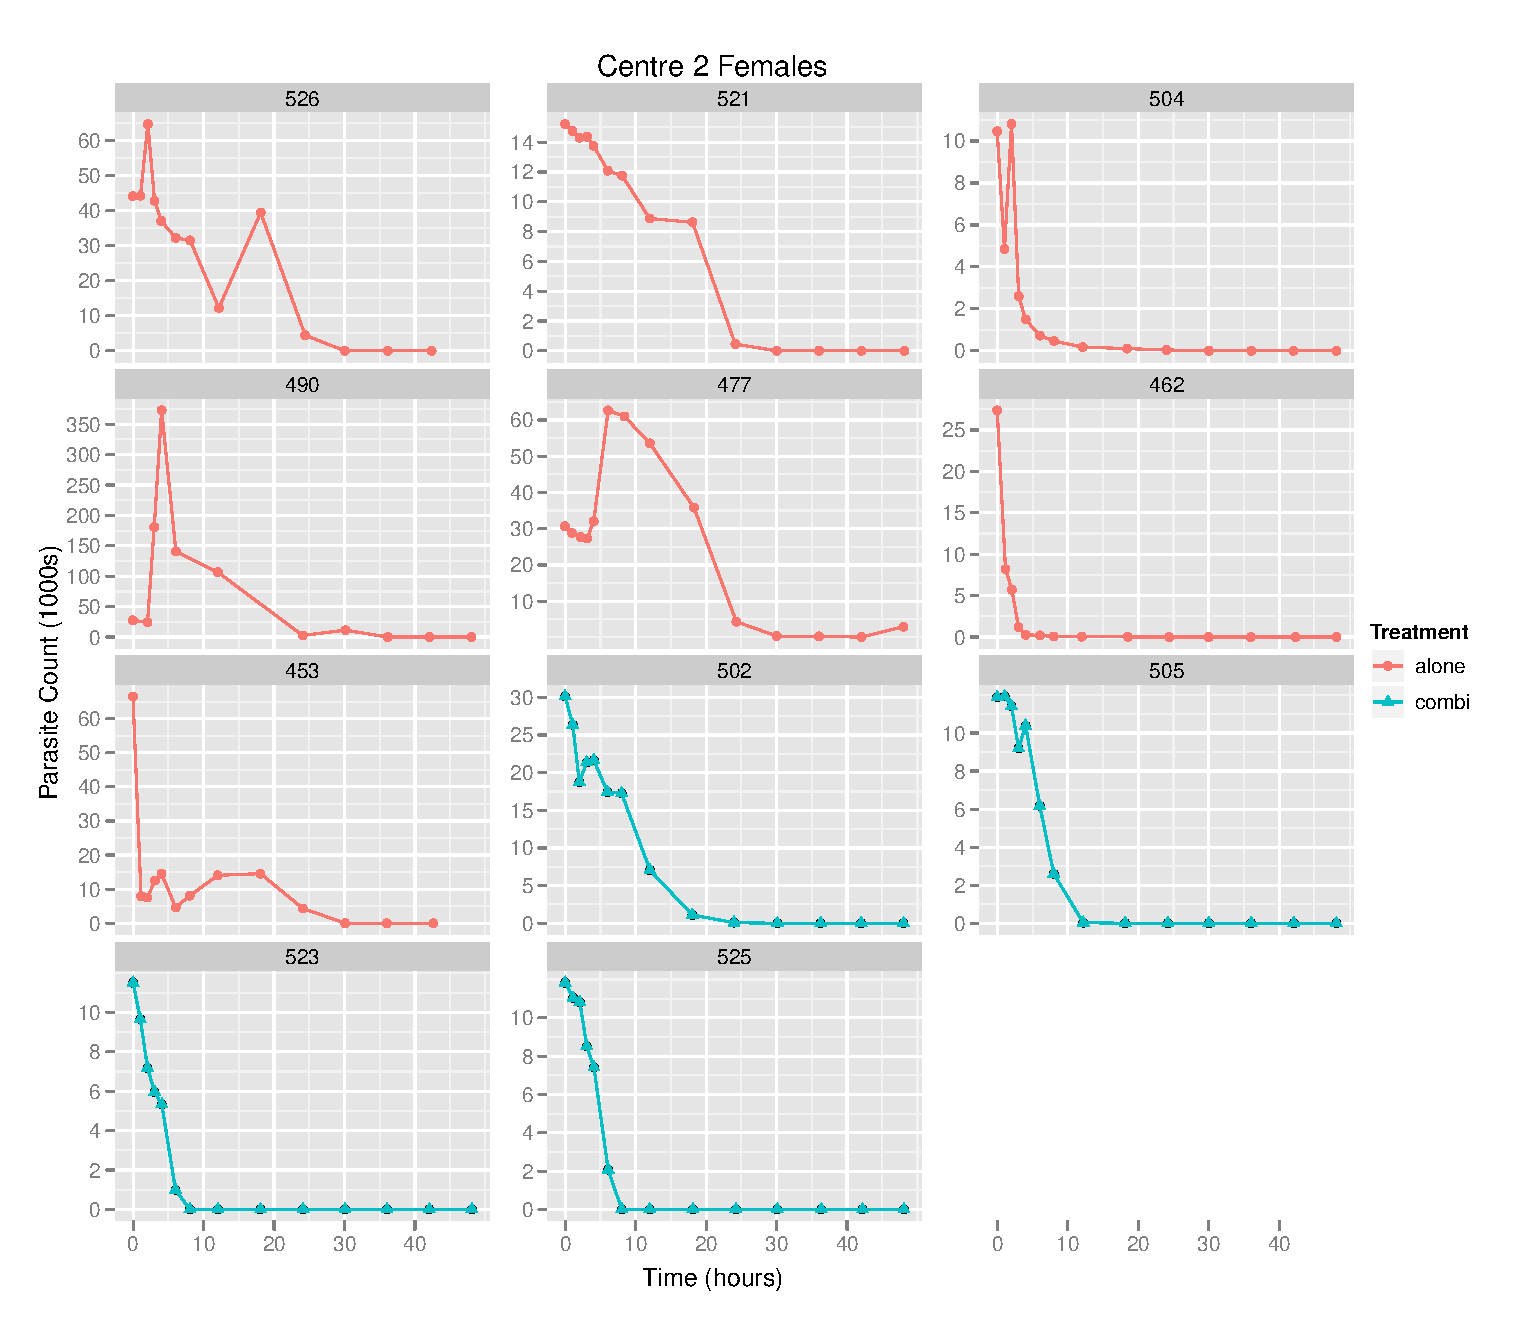
\includegraphics[width=150mm]{raw2f.eps}
%\caption{Parasite count for centre 2 females}\label{raw2F}
%\end{figure} 
%\begin{figure}[h]
%\centering
%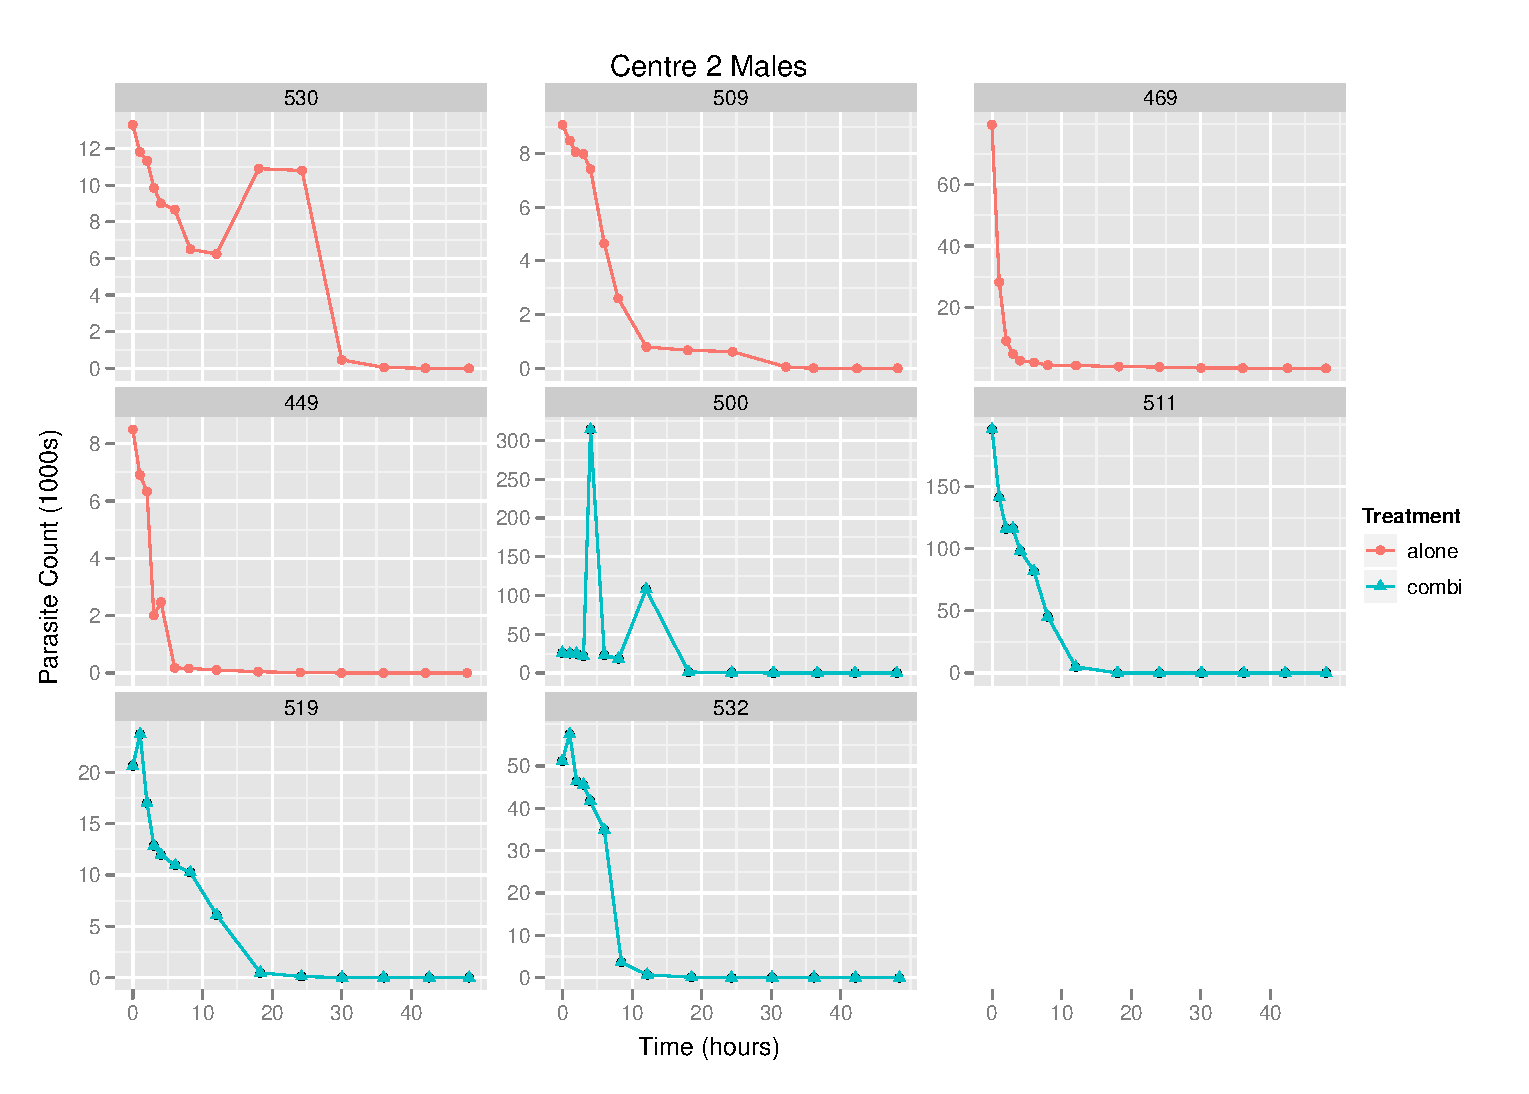
\includegraphics[width=150mm]{raw2m.eps}
%\caption{Parasite count for centre 2 males}\label{raw2M}
%\end{figure} 

\begin{sidewaysfigure}[p]
\centering
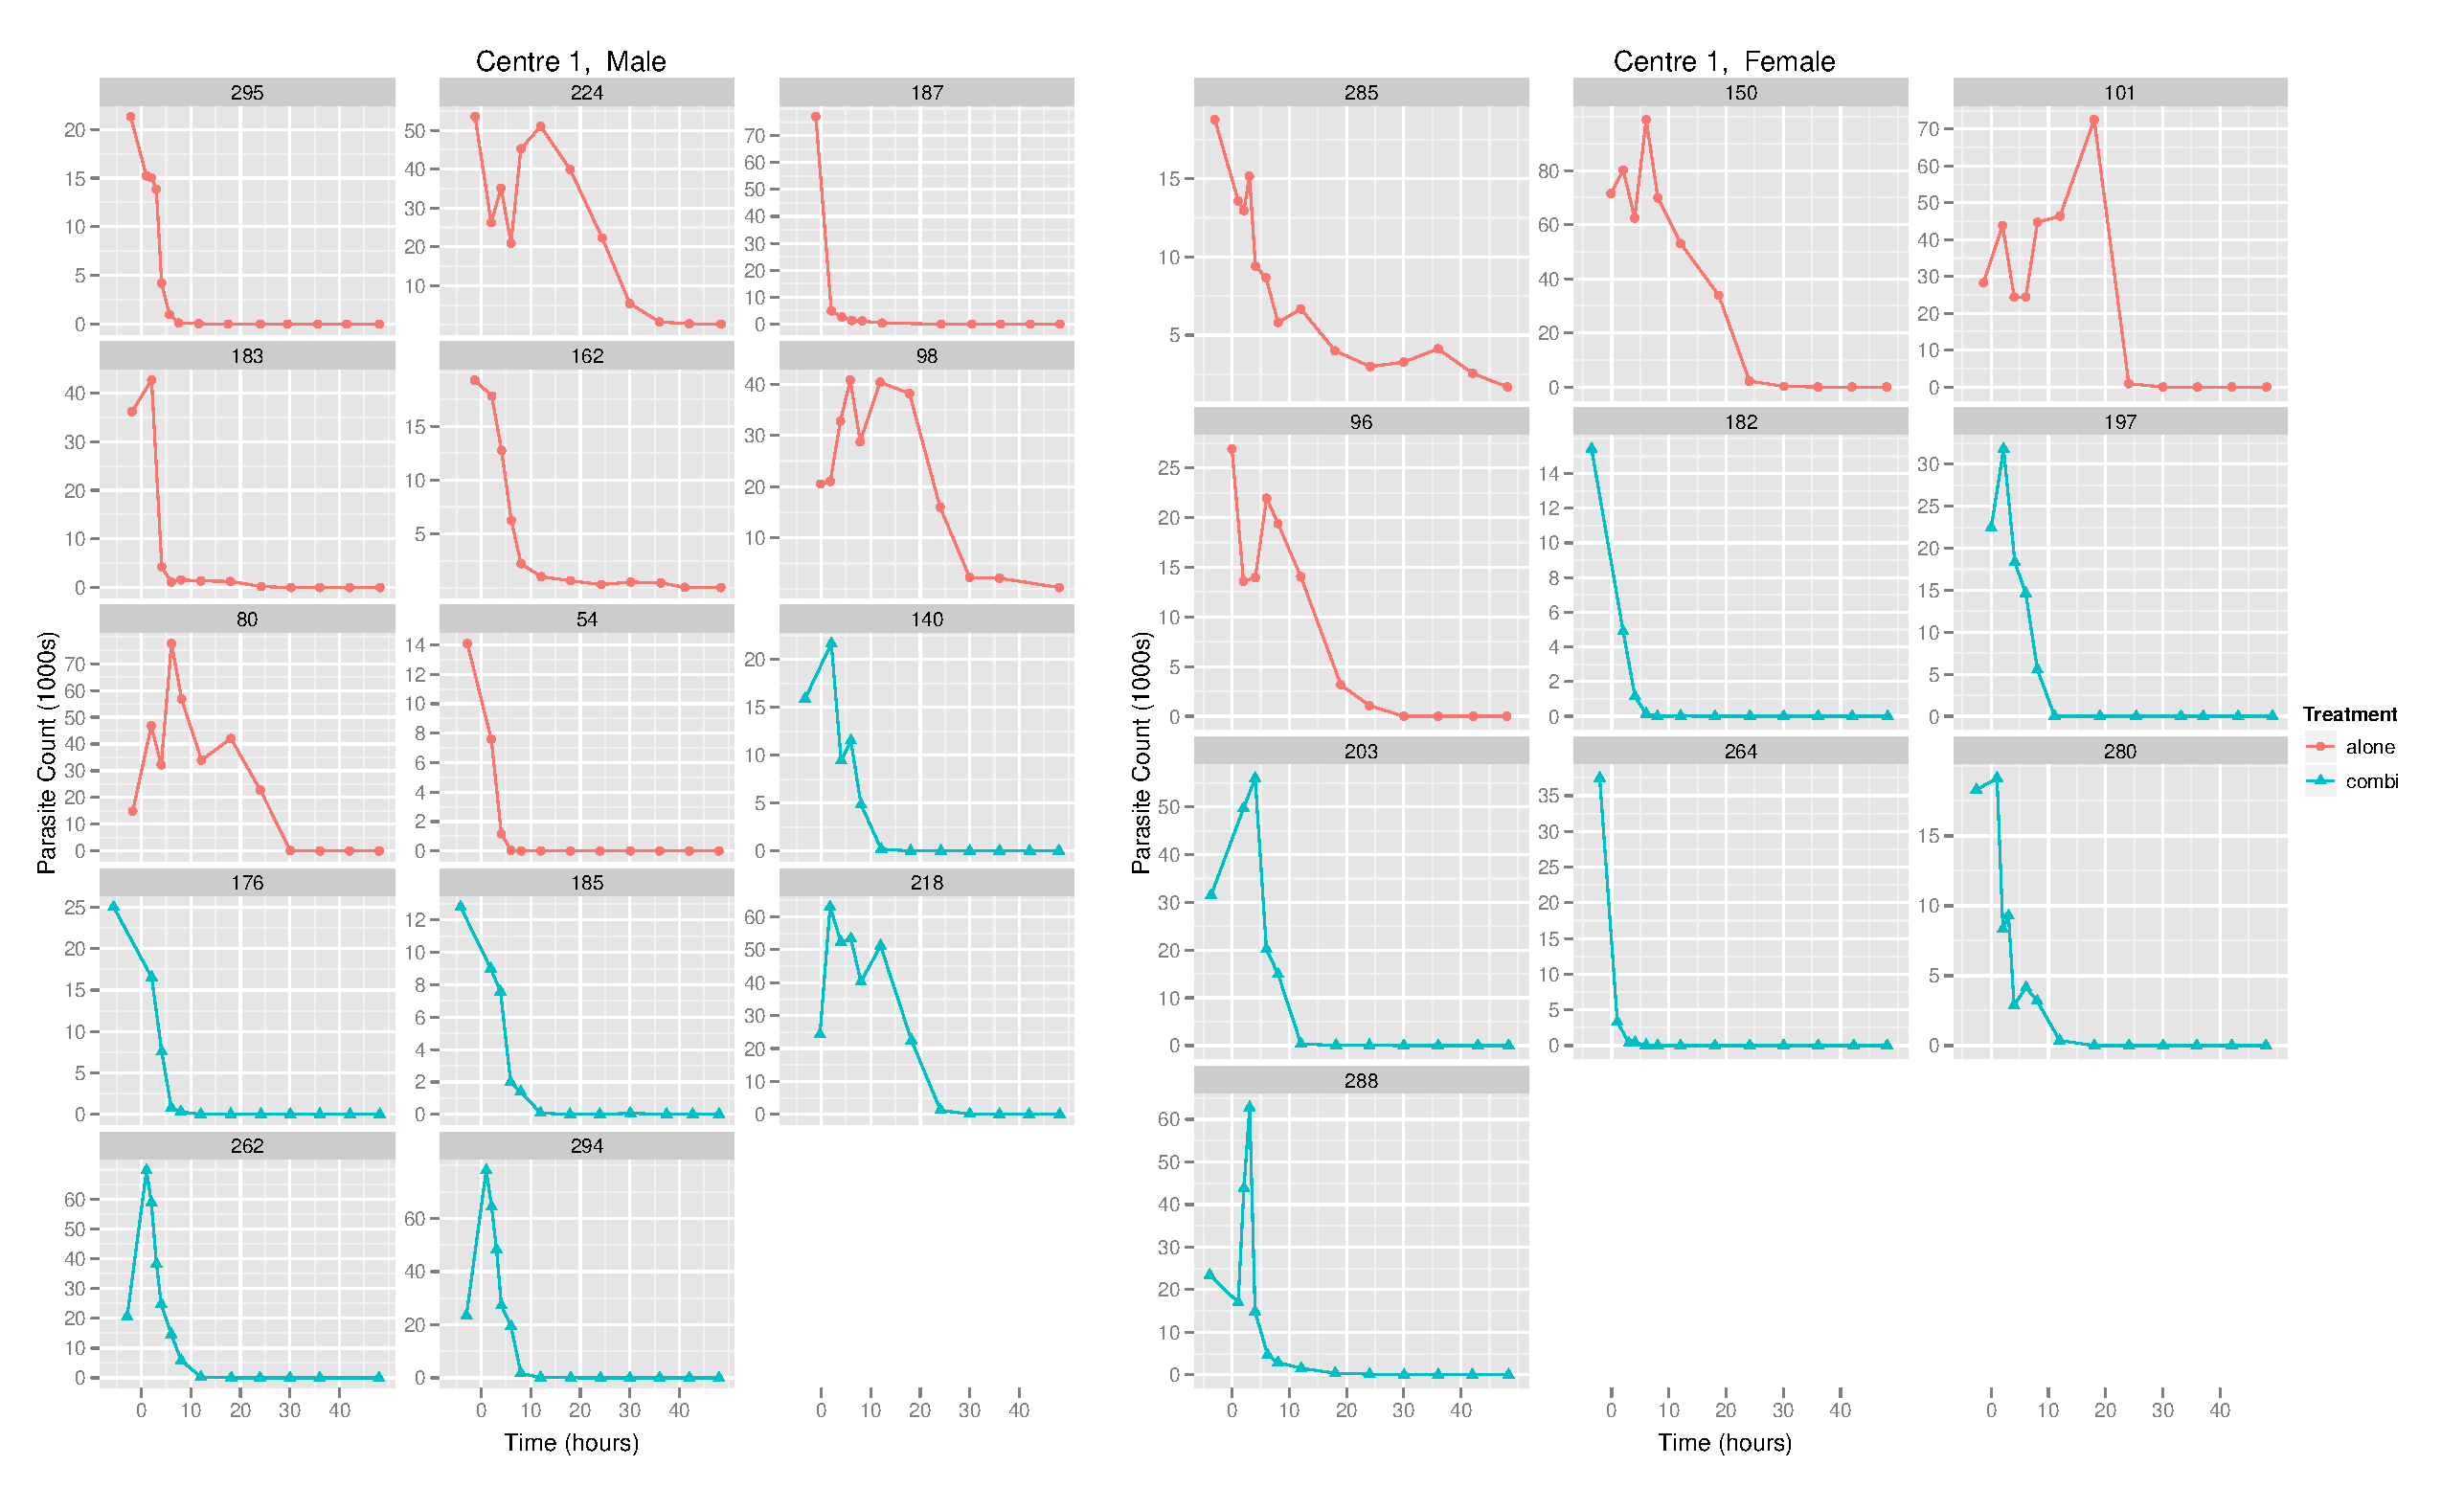
\includegraphics[height=150mm]{raw1.eps}
\caption{Parasite count for centre 1}\label{raw1}
\end{sidewaysfigure} 
\begin{sidewaysfigure}[p]
\centering
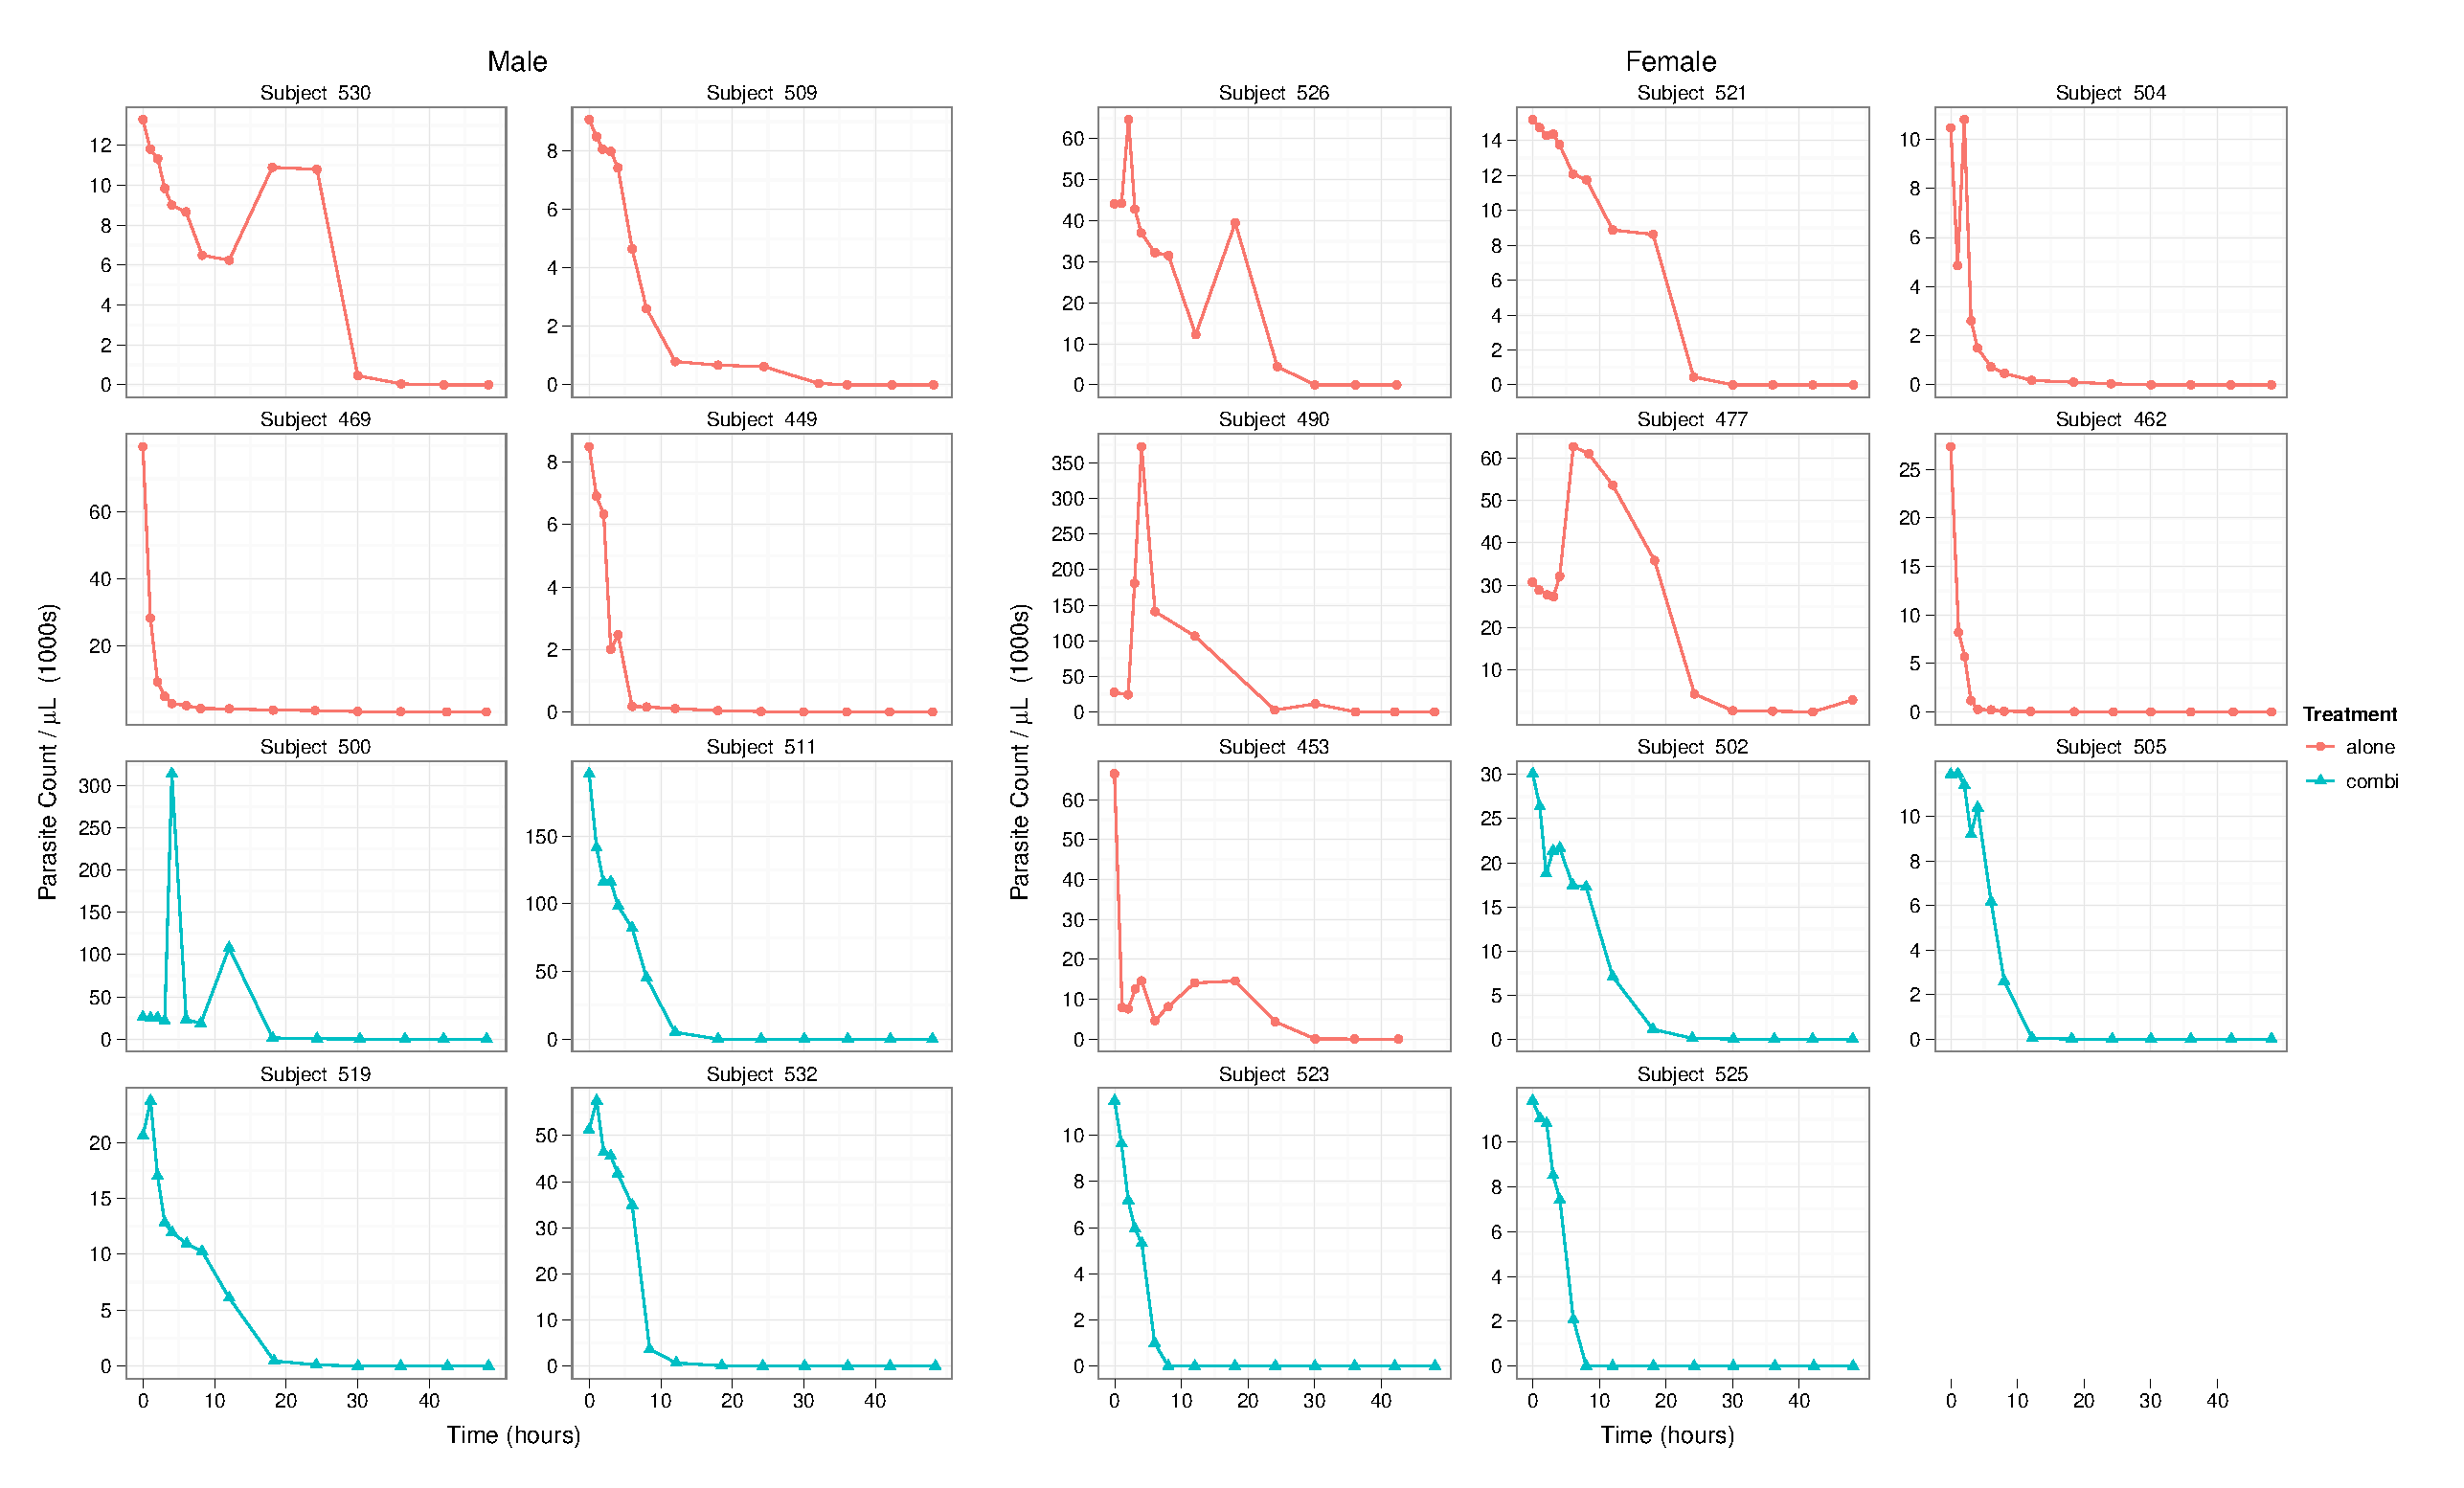
\includegraphics[height=150mm]{raw2.eps}
\caption{Parasite count for centre 2}\label{raw2}
\end{sidewaysfigure} 

\subsection{Main features of the data}
Generally, there appears to be a drop in the parasite count from an initial high level to zero or near zero within about 20 to 30 hours from first treatment. In some cases there is a rapid monotonic drop off within 10 hours. In other cases the \textit{recorded} parasite count fluctuates up and down before dropping to zero over a longer period.

To briefly summarise, the main behaviours observed are:
\begin{itemize}
\item A relatively steep monotonic drop in the count e.g. centre 1 female subjects 182 and 264, centre 1 male subjects 187, 162, 54, 176 and 185 (Figure \ref{raw1}), centre 2 female subjects 462, 523 and 525 and centre 2 male subjects 509, 469 and 511 (Figure \ref{raw2}).

A variation of this type has the parasite count increasing after the first dose before falling e.g. subjects 197 and 203 and subjects 262 and 294 (Figure \ref{raw1}). White\cite{white} notes that ``\textit{parasitemia may rise alarmingly in the hours following treatment}'' and gives reasons therein.
\item A more erratic and slower drop in the parasite count e.g. centre 1 female subjects 285 and 96, centre 1 male subjects 295 and 140 (Figure \ref{raw1}) and centre 2 female subjects 521, 502 and 505 (Figure \ref{raw2}). 
\item The parasite count seems to fluctuate about a constant level before falling e.g. centre 1 female subjects 150 and 101 and centre 1 male subjects 224, 98, 80 and 218 (Figure \ref{raw1}). 
\end{itemize}
There are some profiles that we might suspect contain anomalous data such as subject 500 in Figure \ref{raw2} where there are two unusually high values compared to the main trend. We might suspect that some inconsistency in the counting procedure explains this behaviour rather than the patient's parasite count jumping by a large amount on these occasions. Looking at how the parasite count was obtained should give an insight into potential sources of inconsistency.
\subsection{Implications for modeling}
It can be seen from the parasite count profiles in Figures \ref{raw1} and \ref{raw2} that no simple linear model will closely approximate the behaviour of all patients' counts over the whole time range. However, as we are primarily interested in estimating the time to reduction of the parasite count by 90\% it is only really in this region that it is critical to find a good model. It may be that the erratic behaviour of some parasite counts at short times after first dose is of little relevance. With this in mind, one possible approach may be to use a logarithmic transform of the parasite count thereby emphasising the behaviour at low counts.

\section{Properties of the Parasite Count}

\subsection{Derivation of the Parasite Count}
One of the first questions addressed was whether the parasite count is a true count, and thus Poisson statistics would be applicable, or whether it is a derived measurement. Our contact informed us that the method used to arrive at the parasite count values given is broadly as follows.
\begin{enumerate}
 \item A microscopist would choose ``suitable area'' of a slide of blood and work from left to right counting parasites ($N_p$) and white blood cells ($N_w$).
\item If by the time they have counted around 200 white blood cells they have seen less than 10 parasites then they continue counting until they have counted around 500 white blood cells.
\item The number of white blood cells in a $\mu L$ of blood ($\rho_w$) is automatically counted by a machine.
\end{enumerate}
Accordingly the number of parasites in a $\mu L$ of blood (\texttt{parct}) is given by:
$$\mathtt{parct}=\frac{N_p}{N_w}\rho_w$$
and thus we cannot treat this derived measurement as a count for modeling purposes.

\subsection{The Pre-dose parasite count}
%We were also informed that the white blood cell count is right skewed and so we might expect that the parasite count per $\mu L$ will be also.
%Table \ref{predose} shows the pre-treatment parasite counts in the subjects from each test centre and of each sex. It can be seen that for 3 cases the mean is larger than the median meaning that the distributions are right skewed. This is to be expected for non-negative data such as this. When model fitting to this data we may have to choose some transformation of the parasite count such as taking logarithms.
Figure \ref{preaov} shows the pre-dose parasite counts grouped by sex, centre and treatment. There does not seem to be an obvious dependence of the level of the pre-dose parasite count on sex, centre or treatment, although there appears to be a greater dispersion of the count for patients on the single treatment.
\begin{figure}[p]
\begin{center}
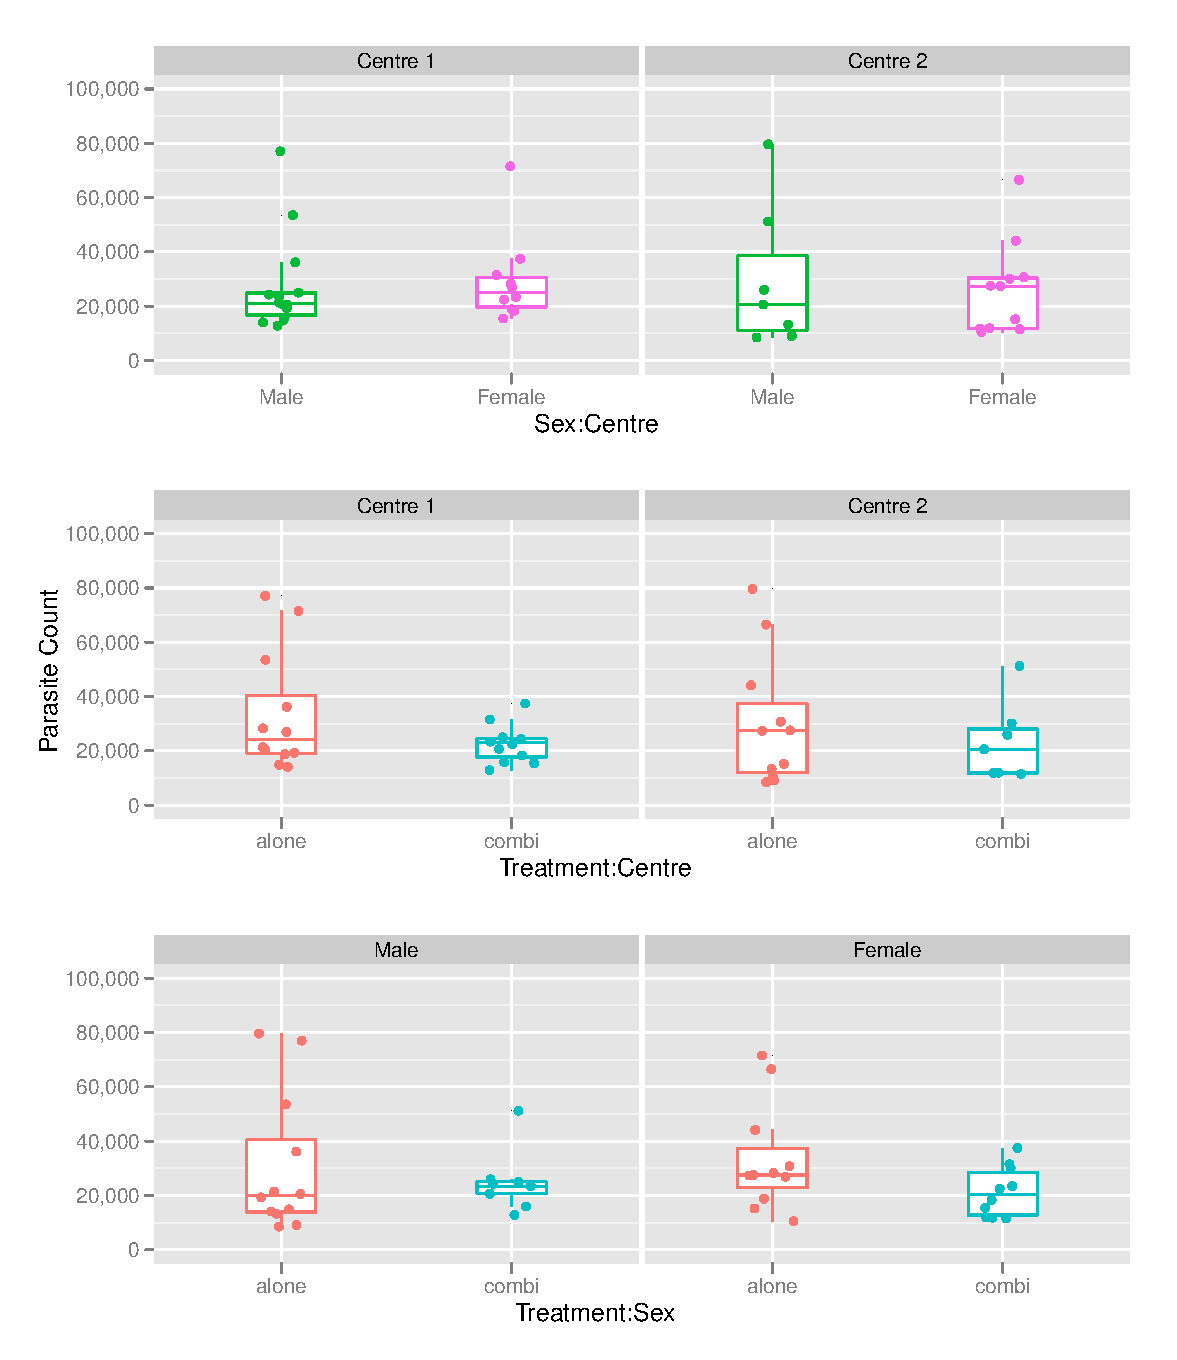
\includegraphics[width=150mm]{preaov.eps}
\caption{Pre-dose parasite counts by sex, centre and treatment, with box plots showing median and quartiles.}
\label{preaov}
\end{center}
\end{figure}

If we perform 3-way ANOVA of the pre-dose parasite count by sex, centre and treatment with all interactions we obtain the residuals shown in Figure \ref{preaovres}. It can be seen that they are right-skewed and heteroscedastic with unstable variance between groups and correlated with fitted parasite count.
\begin{figure}[p]
\begin{center}
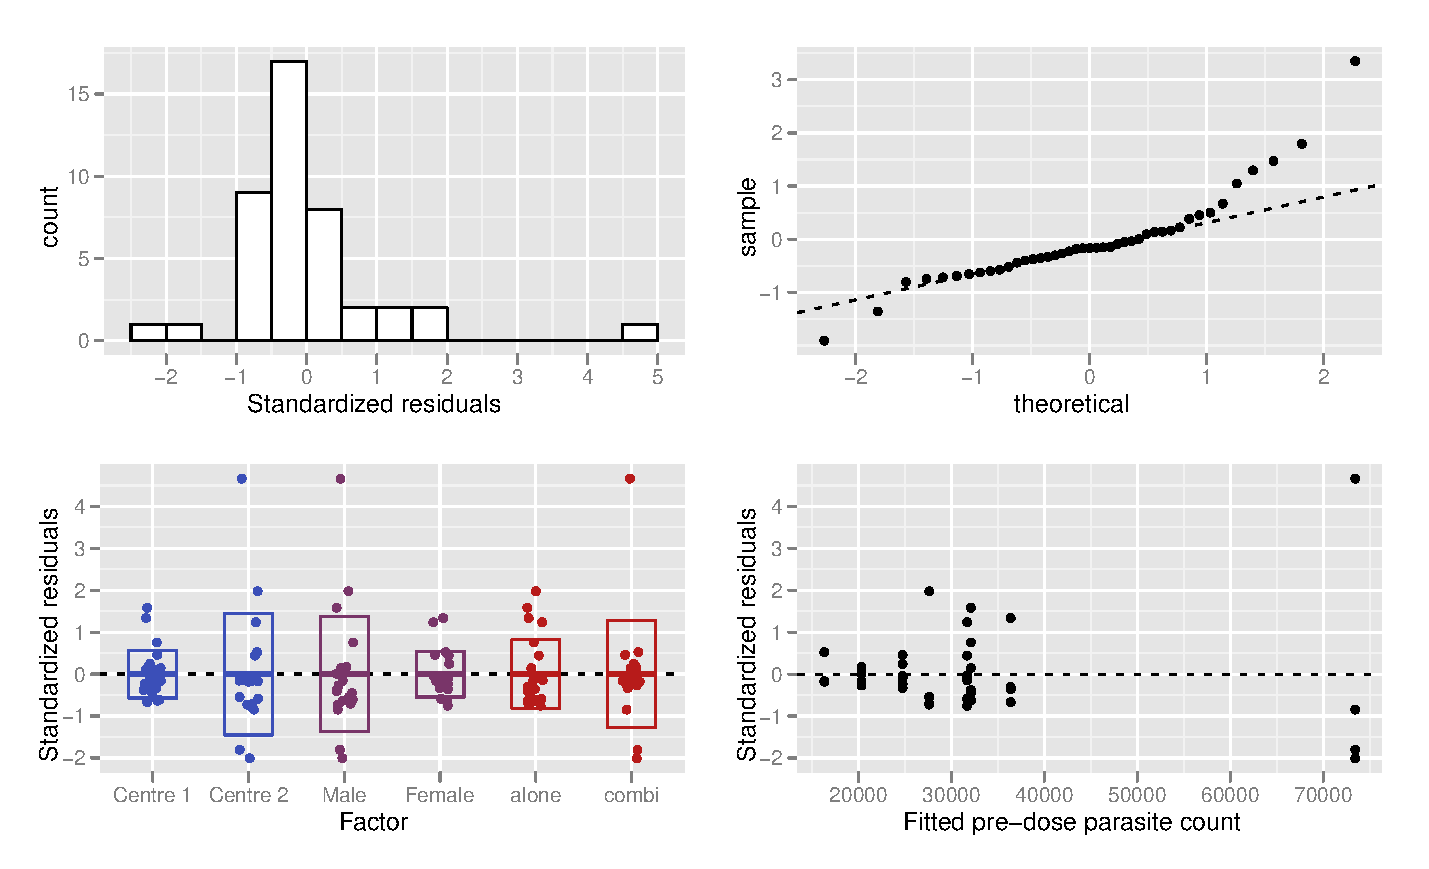
\includegraphics[width=150mm]{preaovres.eps}
\end{center}
\caption{Residuals from 3-way ANOVA of pre-dose parasite counts. Panels from top-left are histogram, QQ normal, residuals vs. factors with mean and $1\sigma$ range shown, residuals vs. fitted values.}
\label{preaovres}
\end{figure} 

If we repeat the ANOVA but with the logarithm of the pre-dose parasite count we find that the residuals are approximately normally distributed and homoscedastic as shown in Figure \ref{logpreaovres}.
\begin{figure}[p]
\begin{center}
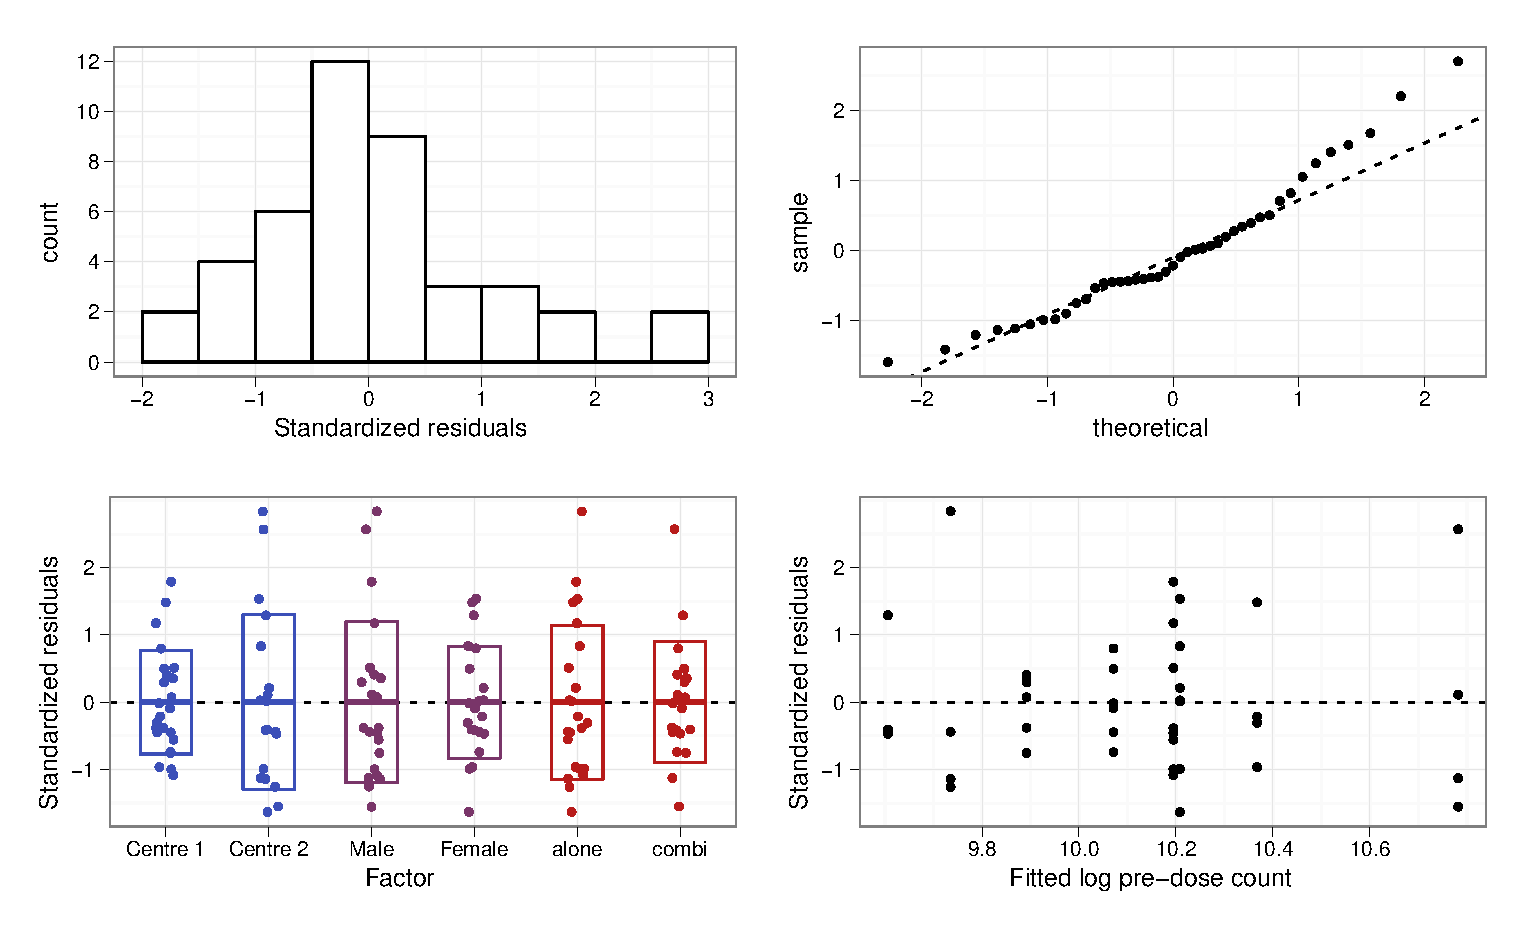
\includegraphics[width=150mm]{logpreaovres.eps}
\end{center}
\caption{Residuals from 3-way ANOVA of log pre-dose parasite counts}
\label{logpreaovres}
\end{figure} 
Using the square-root of the count does not produce as good a normalising transformation: Shapiro-Wilk normality test returns $P<0.0001$ compared to $0.1<P<0.05$ for the logarithmic transformation. The results of the ANOVA analysis are shown in Table \ref{aovpre}.
%                    Df  Sum Sq Mean Sq F value  Pr(>F)  
%CENTREID             1  0.0022  0.0022  0.0055 0.94157  
%SEX                  1  0.0259  0.0259  0.0651 0.80016  
%trttxt               1  0.0722  0.0722  0.1815 0.67273  
%CENTREID:SEX         1  0.4650  0.4650  1.1690 0.28700  
%CENTREID:trttxt      1  0.4580  0.4580  1.1515 0.29058  
%SEX:trttxt           1  1.3336  1.3336  3.3527 0.07562 .
%CENTREID:SEX:trttxt  1  1.7117  1.7117  4.3032 0.04546 *
%Residuals           35 13.9223  0.3978       
\begin{table}[h]
\centering
\caption{ANOVA table for log parasite count at 6 hours after first treatment}\label{aovpre}
\begin{tabular}{l|rrrrrl}
Source&Sum Sq.&df&Mean Sq.&$F$&P($>F$)\\
\hline
$Centre$     &                0.002  &1& 0.002 & 0.006 &0.942&\\
$Sex$        &              0.026  &1& 0.026 & 0.065 &0.800\\
$Treatment$  &            0.072  &1& 0.072  &0.182 &0.672 &\\
$Centre\times Sex$ &             0.465 &1&  0.465 & 1.17 &0.287&\\
$Centre\times Treatment$ &        0.458  &1& 0.458 & 1.15 &0.291&\\
$Sex\times Treatment$     &     1.33  &1& 1.33 & 3.35 &0.076 &\\
$Centre\times Sex\times Treatment$ &  1.71  &1& 1.71 & 4.30 &0.045 &*\\
$Residuals$      &    13.92 &35&  0.398  &&&\\
\hline
Total&17.99&42&&&
\end{tabular}\\
\hspace{20em}*$<0.05$
\end{table}

It can be seen that there is no evidence to reject the hypotheses that none of the factors centre, sex or treatment are related to the pre-dose parasite count, although there is some marginal evidence ($p\approx 0.05$) to reject the hypothesis of no 3-way interaction being present. The Kruskal-Wallis non-parametric equivalent test also does not reveal any evidence of a dependence.
% \begin{table}[h]
% \centering
% \caption{Pre-dose parasite counts}\label{predose}
% \begin{tabular}{|cc|cccccc|}
% \hline
% Centre&Sex&N&Mean&Median&SD&1st Qu.&3rd Qu.\\\hline
% \multirow{2}{*}{001}&M&14&27060&20960&17820.9&16750&24830\\
% &F&10&29410&25170&16221.2&19700&30700\\\hline
% \multirow{3}{*}{002}&M&8&50540&23290&63679.9&12240&58290\\
% %&$M^*$&\textit{7}&\textit{29750}&\textit{20610}&\textit{26436.6}&\textit{11180}&\textit{38580}\\
% &F&11&26110&27360&17262.4&11860&30400\\\hline
% \end{tabular}
% \end{table}

\section{Development of the parasite count with time}\label{sec:develt}
Figure \ref{allaov} shows the progression of the parasite count for all patients with the mean level for each treatment shown.
\begin{figure}[p]
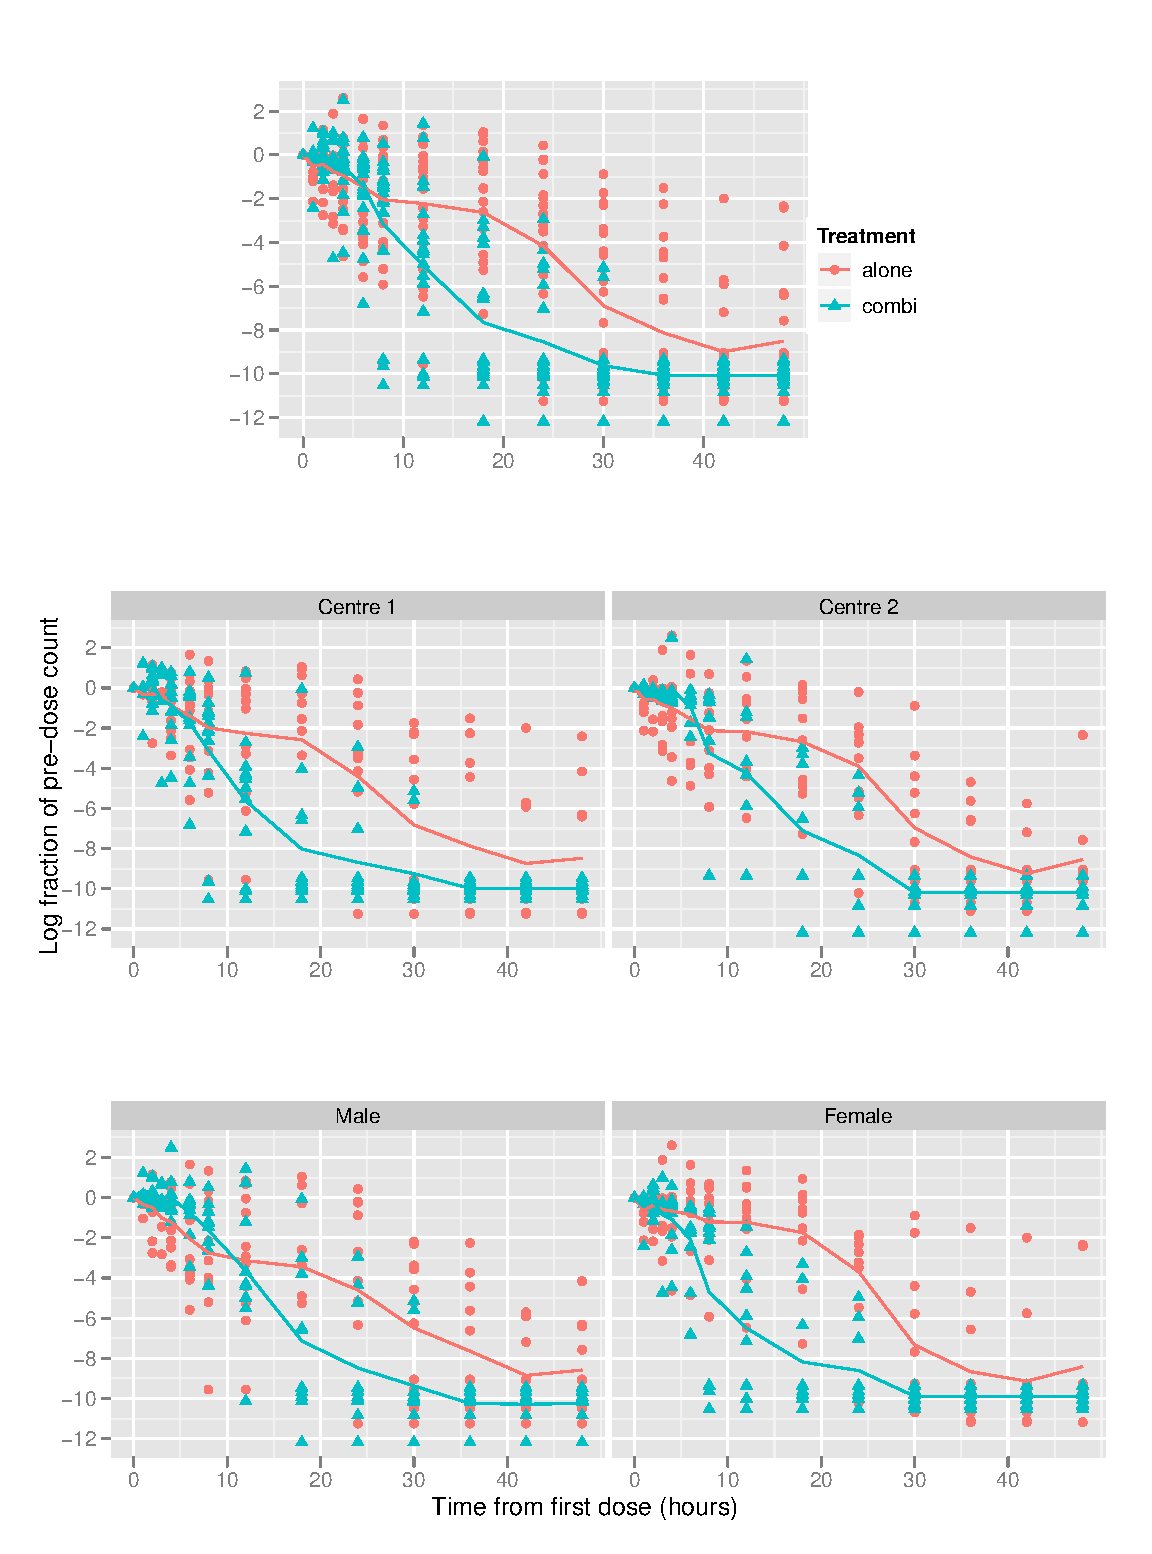
\includegraphics[width=150mm]{allaov.eps}
\caption{Parasite count as proportion of pre-dose count with time from first dose with mean levels shown}
\label{allaov}
\end{figure}
The vertical axis is the logarithm of the fraction of the pre-dose parasite count:
$$y=log\left(\frac{1+P_t}{P_0}\right)$$
where $t$ is the time from first dose and $P_0$ is the pre-dose count. $1+P_t$ is used to avoid problems with taking the logarithm when the parasite count goes to 0. The progression with time is also shown split by centre and then by sex.

With regard to Figure \ref{allaov}, the behaviour as indicated by the average response lines can be summarised as follows:
\begin{itemize}
 \item For female patients on the single-drug (``alone'') treatment the parasite count remains close to the initial level up to about 20 hours from first dose before beginning to fall off.
 \item For male patients on the single-drug treatment the parasite count falls off at a fairly constant rate from first dose, perhaps increasing in fall-off rate after 20 hours.
\item There doesn't seem to be as remarkable a difference between male and female subjects on the combined-drug treatment with parasite counts starting to show an appreciable fall off after about 5 hours in both cases.
\item There is not a readily noticeable difference between centres.
\end{itemize}
In summary it appears from this first rough comparison that the combined treatment is more effective in terms of clearance times than the single treatment. This improvement over the single treatment seems more marked for female patients, but primarily because the single treatment seems to be less effective for female patients with the combined treatment fall-off profile being similar for both sexes.

If we repeat the 3-way ANOVA as for the pre-dose counts but with the logarithm of the counts at 6, 12, 18 an 24 hours from first dose then we find the residuals are normally distributed to a good approximation. The ANOVA analysis shows strong evidence of a dependence of the count on the treatment, which can be seen graphically in Figure \ref{allaov}. We also find at 6 and 12 hours evidence of an interaction between sex and treatment, $P<0.05$ and $P<0.01$ respectively, bearing in mind we are making multiple hypothesis tests and therefore should be more hesitant to draw any early conclusions. At 18 and 24 hours there is no evidence of an interaction with sex, only a treatment effect $P<0.0001$.

The results of the ANOVA analysis at 6 and 24 hours are shown in Tables \ref{aov6} and \ref{aov24}.
%> summary(t6.aov)
%                 Df    Sum Sq   Mean Sq   F value  Pr(>F)  
%SEX               1     0.011     0.011    0.0027 0.95912  
%CENTREID          1     0.810     0.810    0.2055 0.65315  
%trt               1 4.038e-04 4.038e-04    0.0001 0.99198  
%SEX:CENTREID      1     0.110     0.110    0.0278 0.86859  
%SEX:trt           1    26.277    26.277    6.6624 0.01420 *
%CENTREID:trt      1     9.314     9.314    2.3615 0.13336  
%SEX:CENTREID:trt  1 9.205e-05 9.205e-05 2.334e-05 0.99617  
%Residuals        35   138.043     3.944                    
%---
%Signif. codes:  0 �***� 0.001 �**� 0.01 �*� 0.05 �.� 0.1 � � 1        
\begin{table}[h]
\centering
\caption{ANOVA table for log parasite count at 6 hours after first treatment}\label{aov6}
\begin{tabular}{l|rrrrrl}
Source&Sum Sq.&df&Mean Sq.&$F$&P($>F$)\\
\hline
$Sex$     &                0.011  &1& 0.011 & 0.003 &0.959&\\
$Centre$        &              0.810  &1& 0.810 & 0.206 &0.653\\
$Treatment$  &            0.0004  &1& 0.0004  &0.0001 &0.992 &\\
$Centre\times Sex$ &             0.110 &1&  0.110 & 0.028 &0.869&\\
$Sex\times Treatment$ &        26.27  &1& 26.27 & 6.66 &0.014&*\\
$Centre\times Treatment$     &     9.31  &1& 9.31 & 2.36 &0.133 &\\
$Centre\times Sex\times Treatment$ &   $9.2\times 10^{-5}$ &1&  $9.2\times 10^{-5}$ & $2.3\times 10^{-5}$& 0.996&\\
$Residuals$      &    138.04 &35&  3.944  &&&\\
\hline
Total&174.6&42&&&
\end{tabular}\\
\hspace{20em}*$<0.05$
\end{table}
%                 Df Sum Sq Mean Sq F value    Pr(>F)    
%SEX               1   0.87    0.87  0.0885    0.7679    
%CENTREID          1   5.56    5.56  0.5687    0.4558    
%trt               1 209.80  209.80 21.4462 4.865e-05 ***
%SEX:CENTREID      1   8.72    8.72  0.8910    0.3517    
%SEX:trt           1   7.74    7.74  0.7913    0.3798    
%CENTREID:trt      1   1.06    1.06  0.1082    0.7441    
%SEX:CENTREID:trt  1   0.17    0.17  0.0170    0.8971    
%Residuals        35 342.39    9.78          
\begin{table}[h]
\centering
\caption{ANOVA table for log parasite count at 24 hours after first treatment}\label{aov24}
\begin{tabular}{l|rrrrrl}
Source&Sum Sq.&df&Mean Sq.&$F$&P($>F$)\\
\hline
$Sex$     &                0.870  &1& 0.087 & 0.089 &0.768&\\
$Centre$        &              5.56  &1& 5.56 & 0.569 &0.456\\
$Treatment$  &            209.8  &1& 209.8  &21.45 &$4.9\times 10^{-5}$&***\\
$Centre\times Sex$ &             8.72 &1&  8.72 & 0.891 &0.352&\\
$Sex\times Treatment$ &        7.74  &1& 7.74 & 0.791 &0.380&\\
$Centre\times Treatment$     &     1.06  &1& 1.06 & 0.108 &0.744 &\\
$Centre\times Sex\times Treatment$ &   0.17 &1&  0.17 & 0.017& 0.897&\\
$Residuals$      &    342.39 &35&  9.78  &&&\\
\hline
Total&576.3&42&&&
\end{tabular}\\
\hspace{20em}***$<0.0001$
\end{table}
   
We can attempt to get some insight into the interaction of sex and treatment effects by looking at the bottom panel of Figure \ref{allaov}. It appears that there is a greater difference between the treatments for female subjects than for male, with the single-drug treatment parasite count remaining relatively high for female subjects.
\section{Key findings}
Our initial findings after exploratory graphical and preliminary ANOVA analyses are:
\begin{itemize}
\item The parasite data appears to be right-skewed and a logarithmic transformation seems to be appropriate to remedy this. Wootton \textit{et al.}\cite{wootton} chose a logarithmic transformation of the parasite count in their study of similar data.
\item The pre-dose parasite count does not seem to be related to sex, centre or intended treatment or combinations of these.
\item The parasite count after treatment shows dependence on the treatment with possibly some interaction with the sex of the subject at early time points.
\end{itemize}

In the next chapter we will go on to look at how to estimate the endpoint of primary importance for subjects, the time to reduce the parasite count by 90\%.
\chapter{Derivation of Parasite Clearance Times}\label{ch:derivation}
\section{Estimating the primary endpoint}
The endpoint of primary importance is PC90, the time to achieve a reduction of the parasitaemia by 90\% from the baseline level. The baseline level is the pre-dose parasite count. We have data for parasite counts taken at approximately fixed times after first dose. Therefore we will have a measurement of the parasite count at a time when the count was above 10\% of the baseline count, followed by one where it where it is below 10\% and hence we need to find an appropriate interpolation to determine a time at which the parasite count was 10\% of baseline i.e. has fallen by 90\%.

As a first attempt at deriving estimates of PC90 from the data, simple linear polynomial fits to the logarithm of the parasite count with time from first dose are investigated. This is followed by non-linear logistic regression as has been used by others\cite{wootton}. We also look at simple linear log-linear interpolation\footnote{Linear interpolation between two points plotted in cartesian co-ordinates where one axis has a logarithmic scale.}, which has also been used for data of this kind\cite{carmello}.
\subsection{Using a transformation of the count}
In the previous chapter it was noted that a logarithmic transformation was appropriate to remove the skew of the parasite count distribution. Figure \ref{comprawlog} shows the untransformed parasite count for centre 1 males with a horizontal line indicating the PC90 level on the left, with the corresponding log-transformed parasite count on the right.
\begin{sidewaysfigure}[p]
\begin{center}
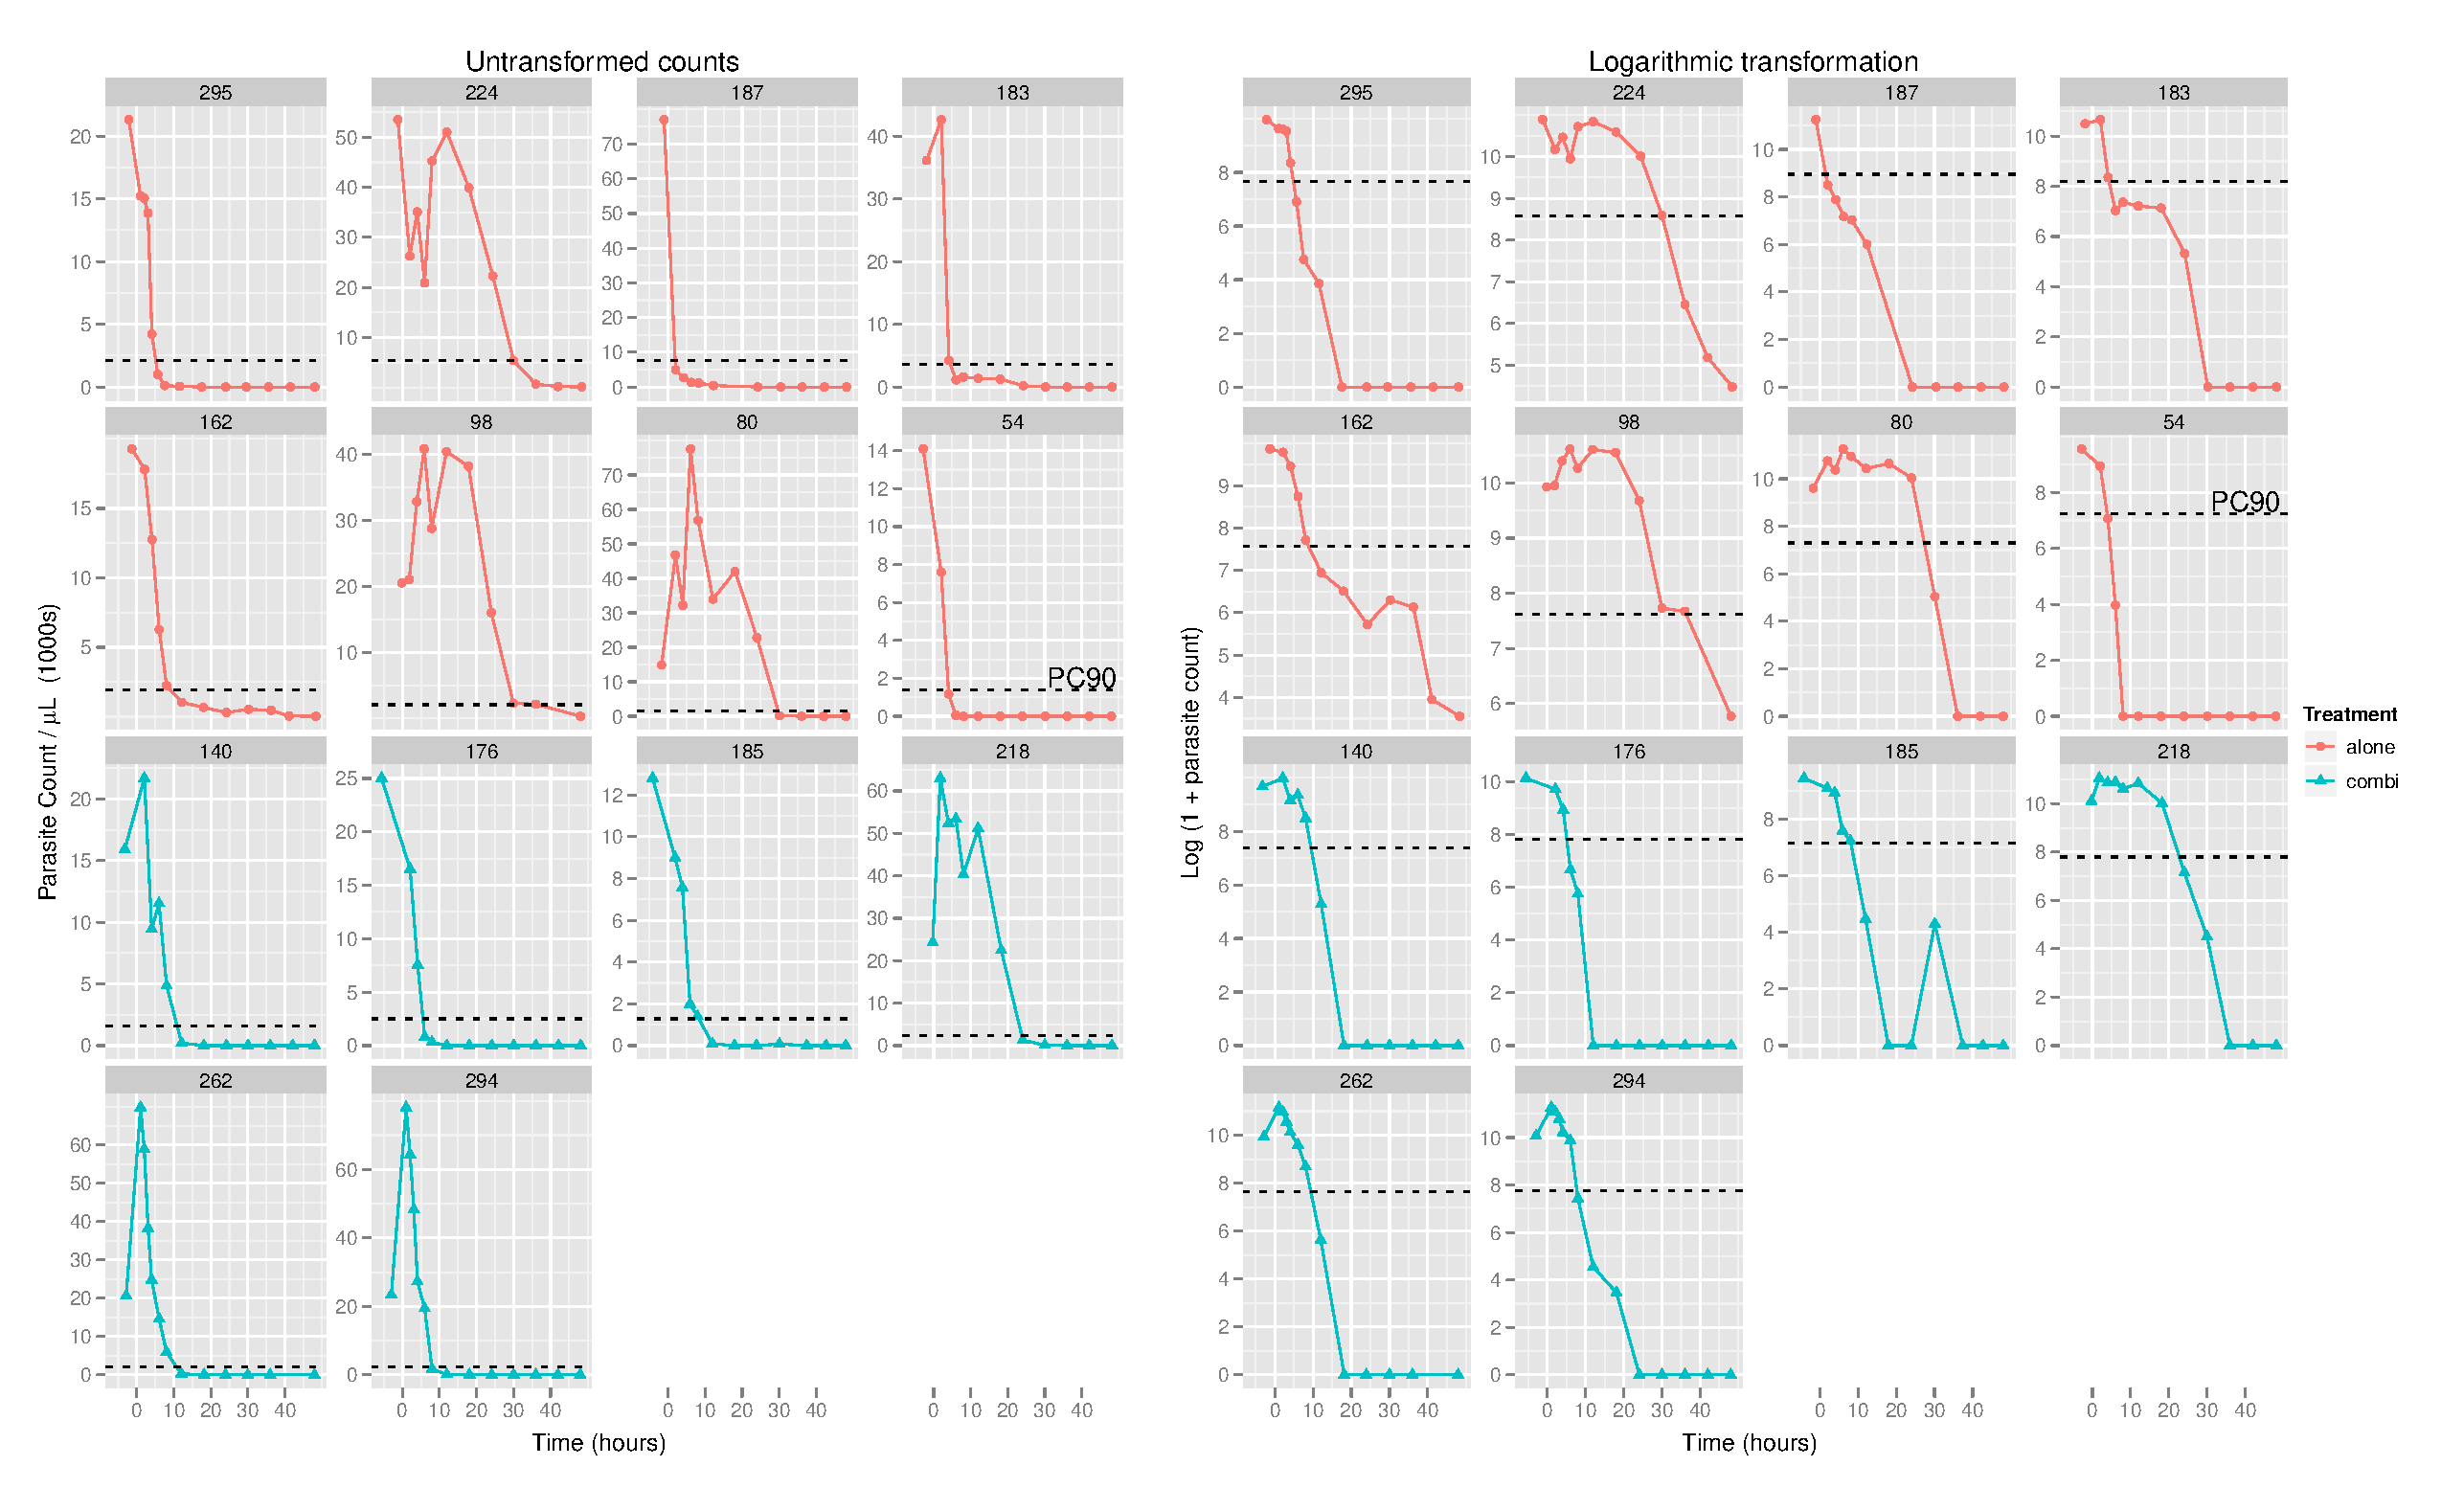
\includegraphics[height=150mm]{comprawlog90.eps}
\caption{Comparison of using untransformed counts and logarithmic transformation for estimation of PC90}
\label{comprawlog}
\end{center}
\end{sidewaysfigure}

We can see that the logarithmic transformation reduces the significance of large fluctuations in the parasite count soon after first dose and brings the region around the PC90 level into greater prominence. Consequently, interpolated estimates of PC90 in these log-linear co-ordinates will be more accurate and any regression will be more influenced by data close to the region of interest.  

\section{Estimation techniques}
\subsection{Polynomial linear regression}
It was found that a cubic polynomial was the most suitable model, if we include the data only up to the first zero parasite count. For some patients where the parasite count drops quickly to zero a fit that includes the subsequent run of zeroes would pull the cubic fit away from the most sensible estimate of PC90. It is more suitable for the purpose of estimating PC90 to only model the drop in the count to zero.

A cubic model was fitted to the log-transformed parasite count $P_{t}$ with time from first dose $t$ as the explanatory variable thus
$$\log(1+P_{t})=\beta_0+\beta_1t+\beta_2t^2+\beta_3t^3+\epsilon\quad\quad\epsilon\sim N(0,\sigma^2)$$
where $\log(1+P_{t})$ is used so that the dependent variable is zero at zero parasite count.

Figure \ref{cubics} shows the cubic fits to the log parasite count for centre 1, male subjects. It can be seen that the model describes the data fairly well, but it looks as if the combined treatment data is more closely modelled, with the single treatment data showing more dispersion about the fitted model. 
\begin{figure}[h]
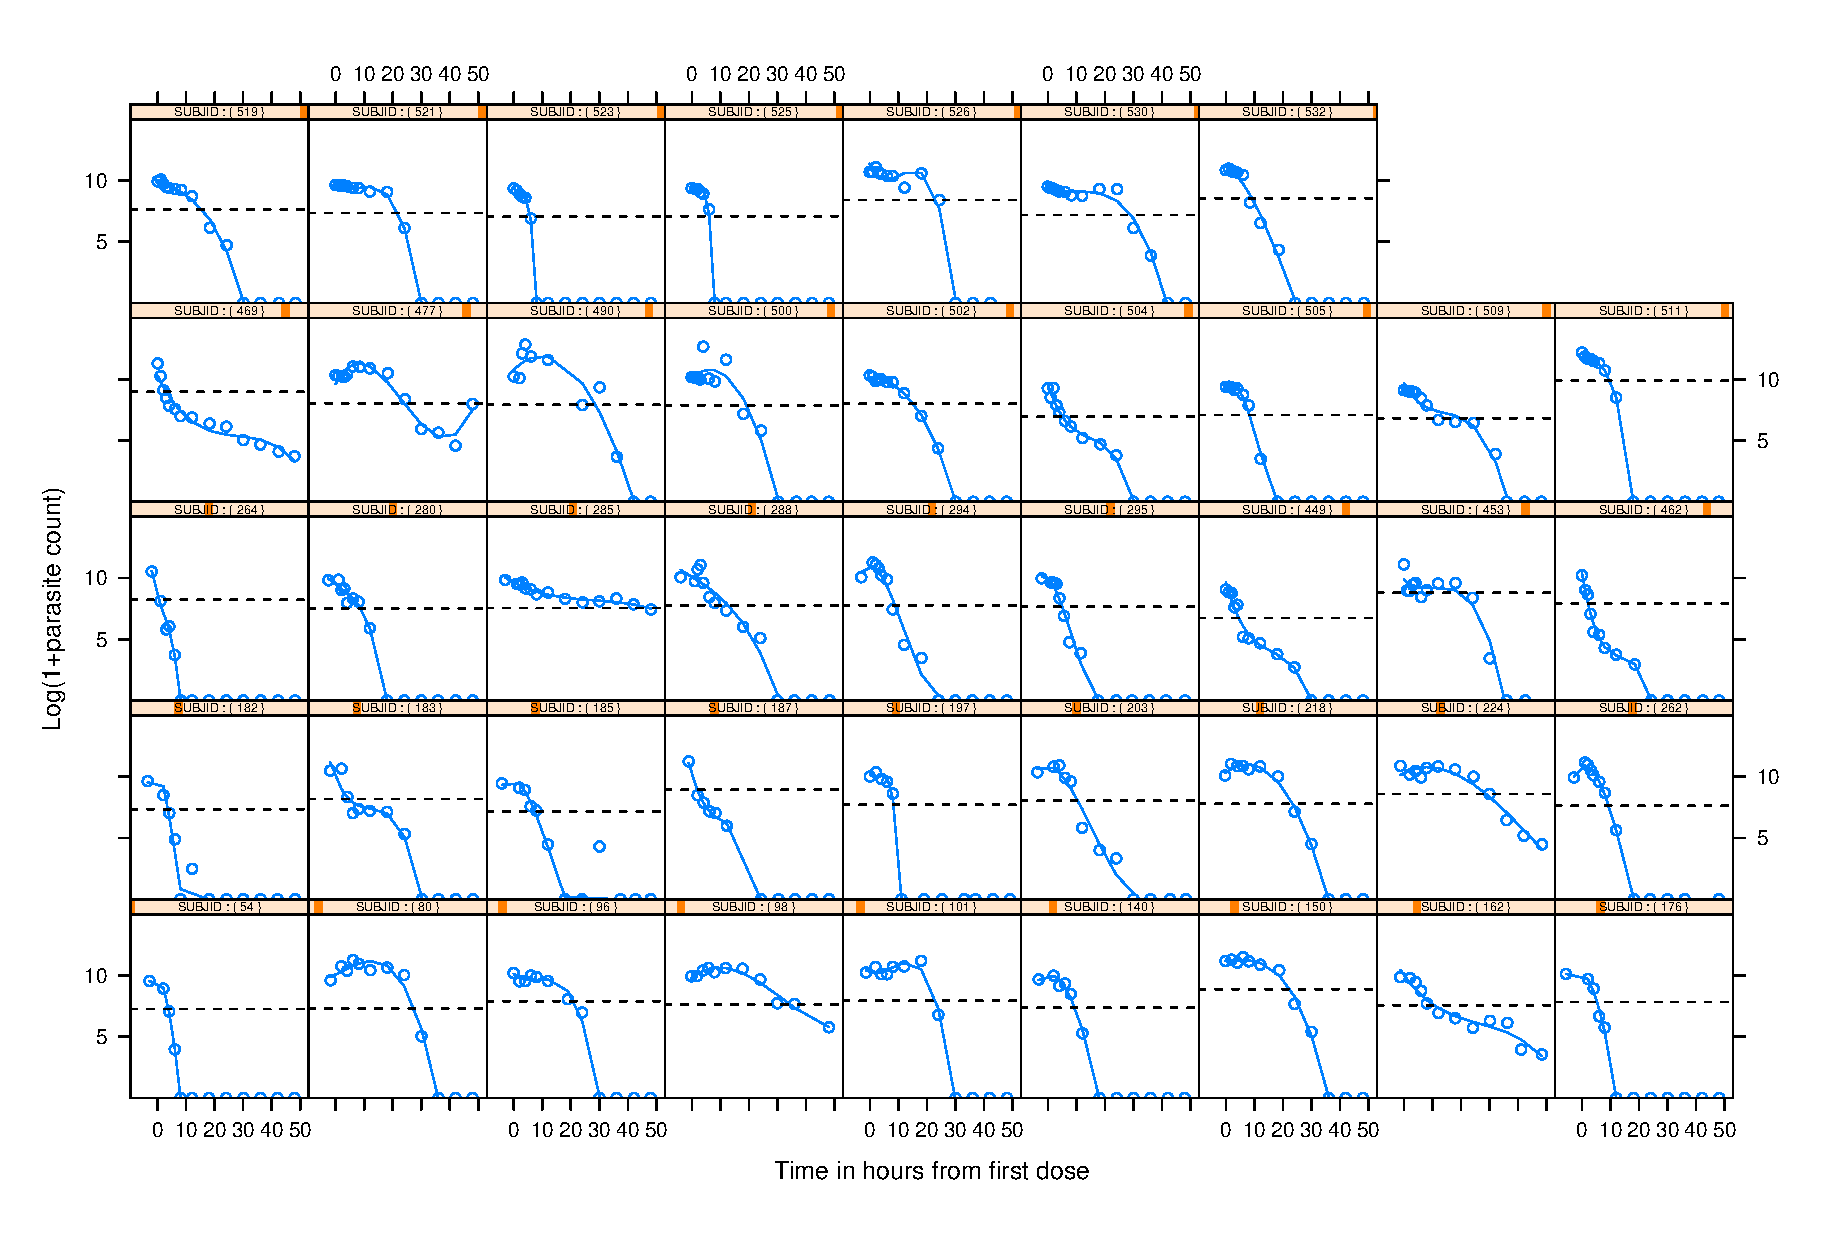
\includegraphics[width=150mm]{cubics.eps} 
\caption{Cubic fits to log parasite count up to first zero reading}\label{cubics}
\end{figure}

Figure \ref{cubicsresid} shows the standardized residuals ($e/\hat{\sigma}$) for the cubic fits.
\begin{figure}[h]
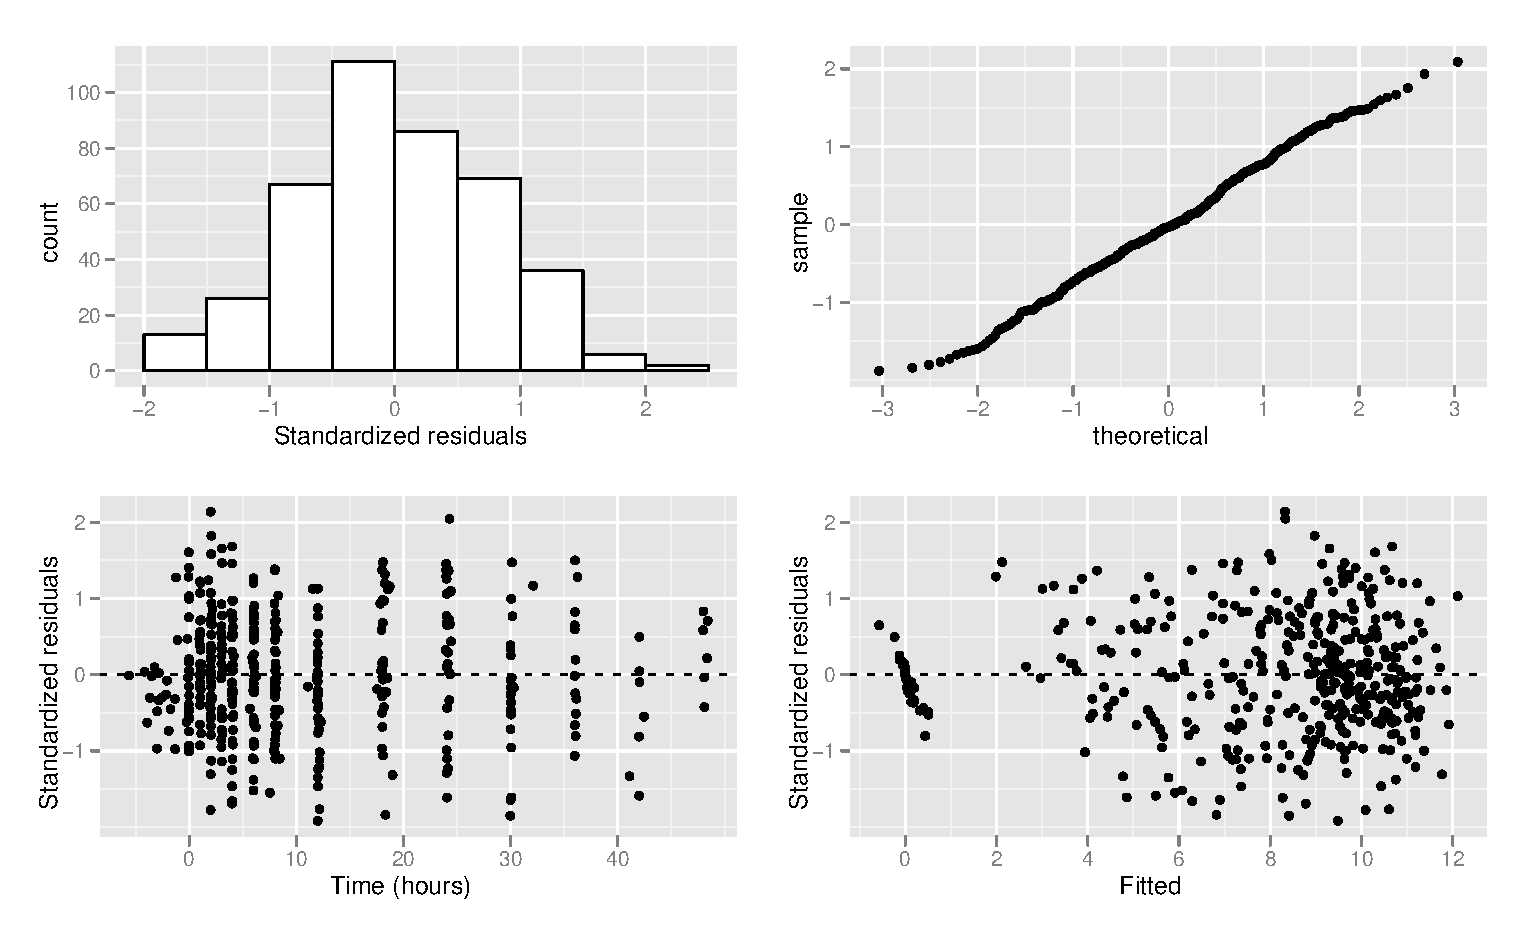
\includegraphics[width=150mm]{cubicsresid.eps} 
\caption{Standardized residuals for cubic fits}\label{cubicsresid}
\end{figure}
It can be seen that they are normally distributed and show no obvious correlation with time from first dose or with fitted count. The cluster of small magnitude residuals at zero fitted value occurs because, in the fitting, this datum is not random but always zero each subject. Strictly this invalidates the assumptions of the fitted model but there isn't a more suitable choice for determining the shape. The cubic model is really only used as a convenient method of interpolation and we are not interested in inference regarding the fitted parameters as long as there is no systematic bias. 

\subsubsection*{Determining PC90 from the fitted model}
The value of PC90 i.e. the time t at which the parasite count has fallen to 10\% was found by finding the positive root of the cubic equation
$$\hat{\beta_0}-\hat{\beta_1}t-\hat{\beta_2}t^2-\hat{\beta}_3t^3-0.1{P_{0}}=0$$
that lies within our time period, where $P_0$ is the pre-treatment parasite count, $t$ is the time from first dose and $\hat{\beta_i}$ are the fitted coefficients for the cubic model. This root was found numerically using the \emph{R} \texttt{uniroot} function\cite{R}, which takes as an argument the interval over which to search for the root.

\subsection{Non-linear logistic regression}
The logistic model that GSK specified had been tried for this data and also used by Wootton \textit{et al}.\cite{wootton}, is
$$\log(1+P_t)=\alpha+\frac{\lambda}{1+e^{-\beta(t-\mu)}}+\epsilon\quad\quad\epsilon\sim N(0,\sigma^2)$$
This was fitted to all the data as it can model a drop from an initial count level to a level of zero, unlike the cubic model. $\alpha$ is the lower asymptote which we would expect to be zero. $\alpha+\lambda$ is the upper asymptote which we would generally expect to be $P_0$ except in the cases where there is a marked increase in the parasite count after the first dose. $\beta$ determines the rate of reduction with time and $\mu$ is the point of inflection (maximum rate of reduction). This model was fitted using the \emph{R} non-linear least-squares function \texttt{nls}\cite{R}. Logistic fits to the same subjects as the cubic fits in Figure \ref{cubics} are shown in Figure \ref{logistics}.
\begin{figure}[h]
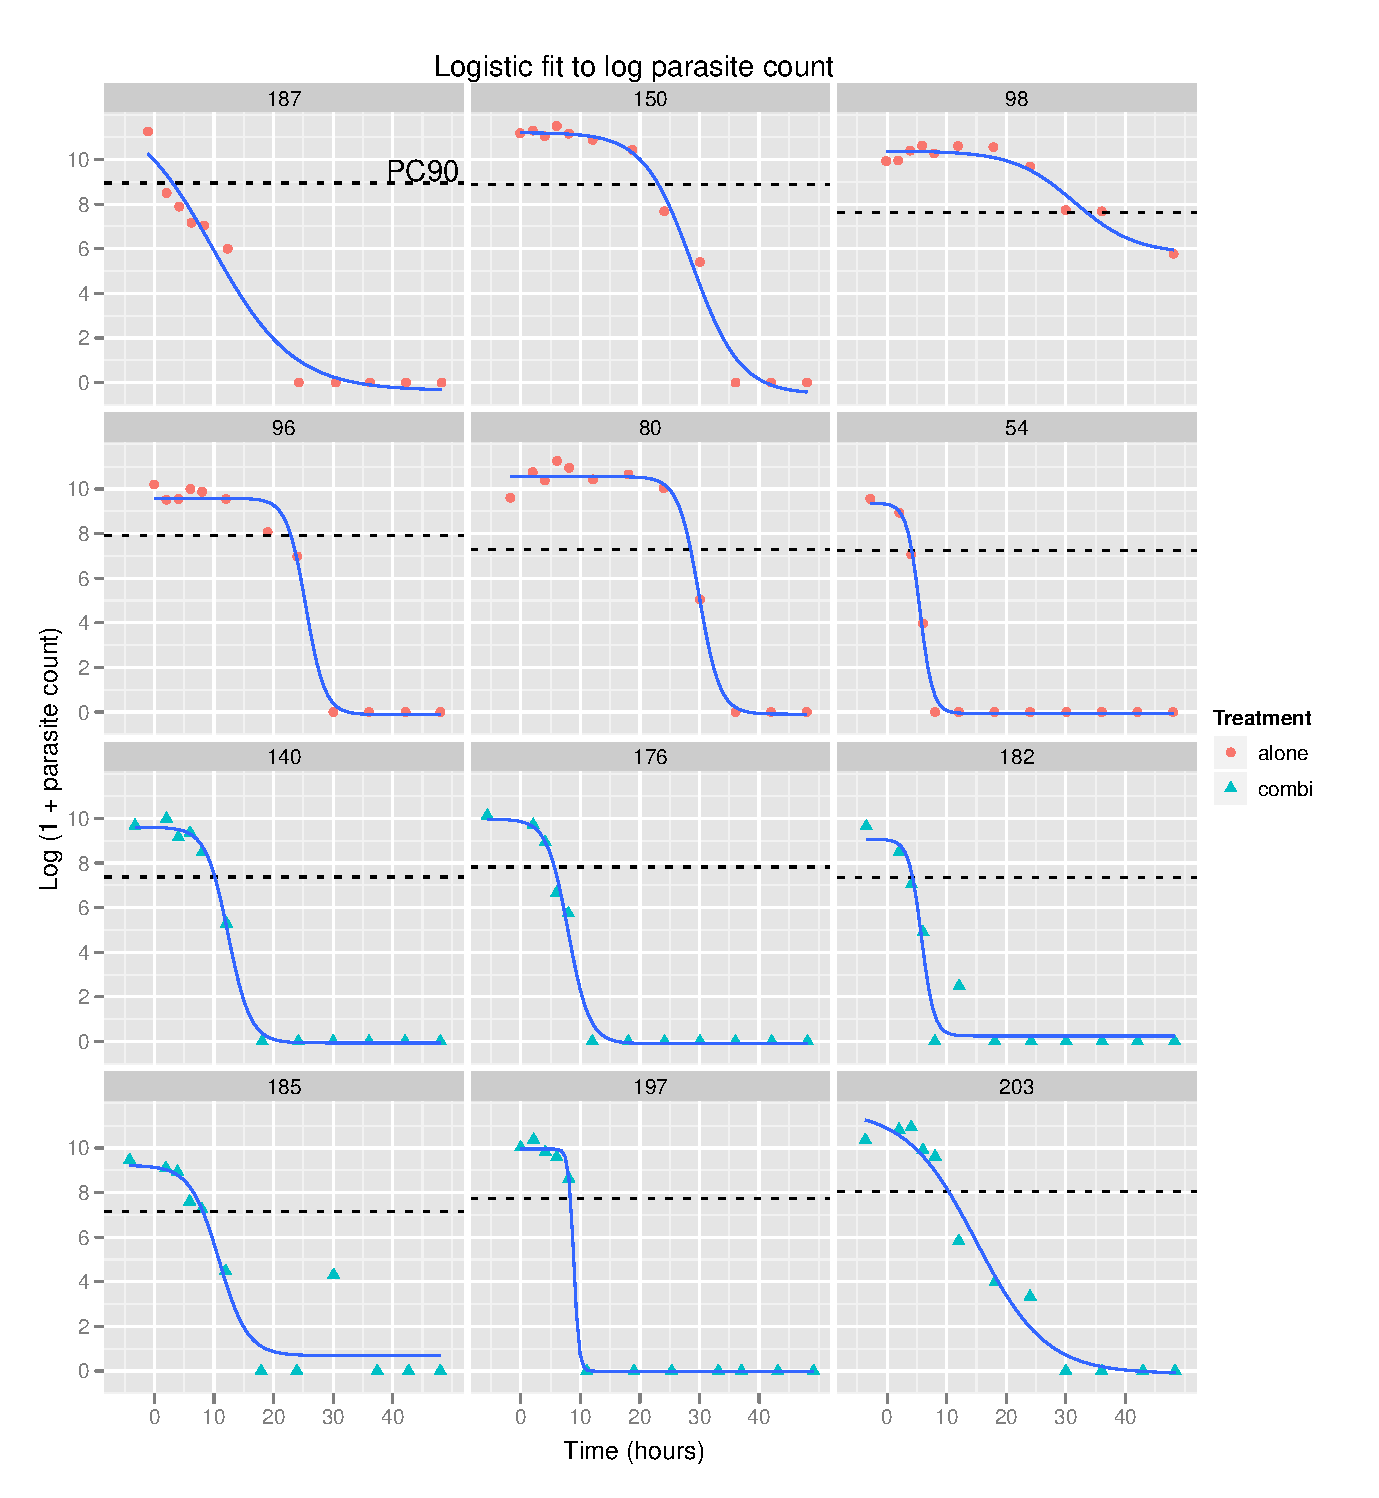
\includegraphics[width=150mm]{logistics.eps} 
\caption{Logistic fits to log parasite count}\label{logistics}
\end{figure}

It can be seen that the logistic model describes the data about as well as the cubic model for these subjects except perhaps slightly worse for subject 96 and slightly better for subject 80.

If we look at the standardized residuals from the logistic fitting in Figure \ref{logisticresid} we can see that the logistic model is not an appropriate statistical model for this data. The residuals are not normally distributed and they are correlated with time and fitted parasite count. Again, inclusion of the run of non-random zero counts is partially responsible for this. However, this does not entirely invalidate this approach as all we are really concerned with here is a method that will automatically give us a sensible PC90 estimate in the region of interest; formulating an appropriate statistical model of the behaviour over the whole time period not the aim here.
\begin{figure}[h]
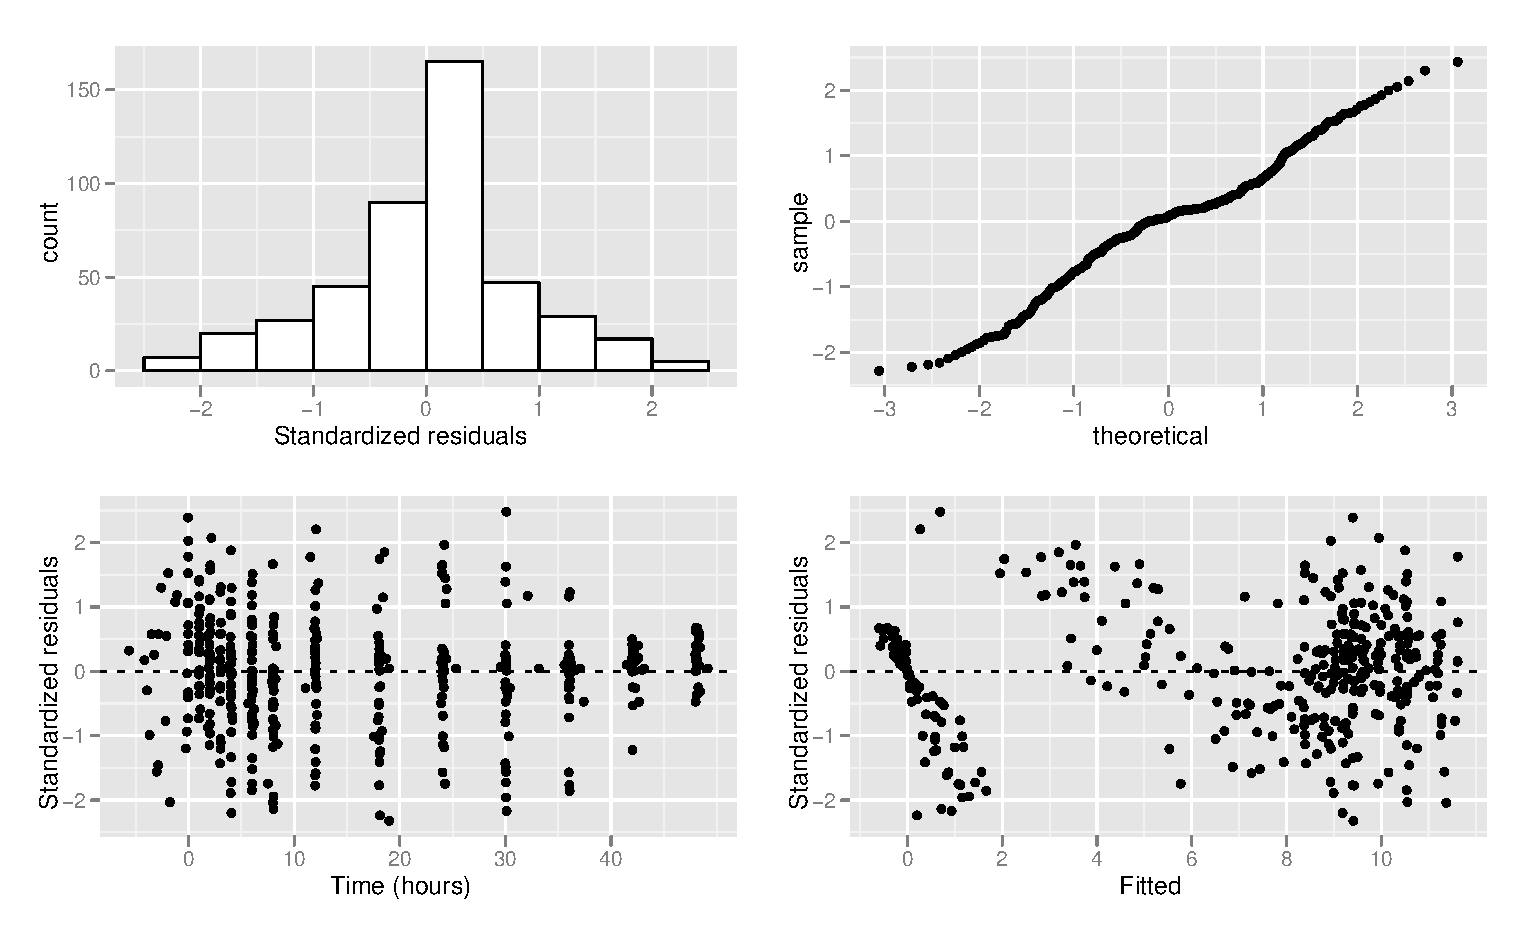
\includegraphics[width=150mm]{logisticresid.eps} 
\caption{Standardized residuals for logistic fits}\label{logisticresid}
\end{figure}

\subsubsection*{Determining PC90 from the fitted model}
As before the \emph{R} \texttt{uniroot} function was used to find $t$ lying within our time period satisfying the equation
$$\log(1+P_t)=\hat{\alpha}+\frac{\hat{\lambda}}{1+\exp[-\hat{\beta}(t-\hat{\mu})]}-0.1{P_{0}}=0$$
where $\hat{\alpha}$, $\hat{\lambda}$, $\hat{\beta}$ and $\hat{\mu}$ are the fitted coefficients of the model.
\subsubsection*{Choosing starting values for the parameters}
Figure \ref{logparms} shows the roles the parameters of the logistic model play in shaping the fitted curve. The \texttt{nls} non-linear, least-squares fitting routine can take starting values for the parameters to be estimated.
\begin{figure}[ht]
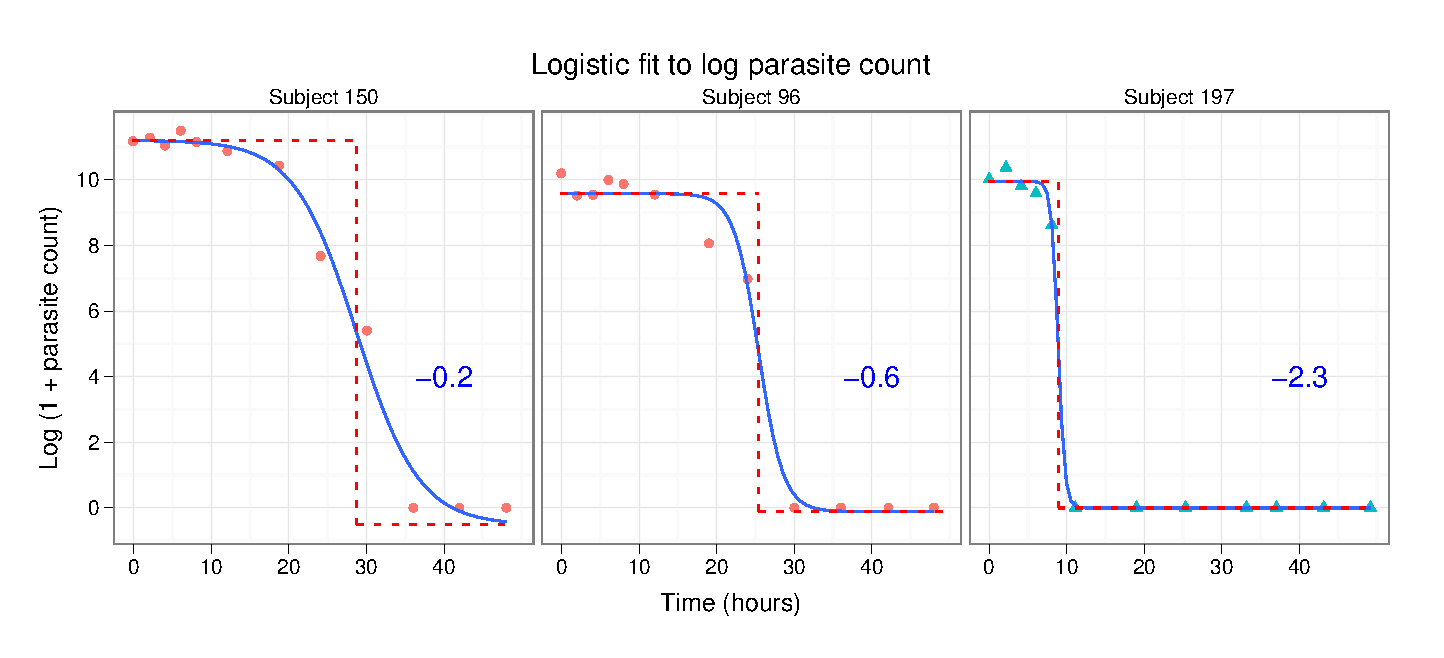
\includegraphics[width=150mm]{logparms.eps} 
\caption{Illustration of parameters for logistic fits.\newline
The horizontal red lines show $\log(1+P_t)=\alpha$ (lower) and $\log(1+P_t)=\alpha+\lambda$ (upper), the vertical red line shows $t=\mu$ and the coefficient $\beta$ (rate of reduction) is given in blue.}\label{logparms}
\end{figure}

Looking at Figure \ref{logparms} it clearly follows that sensible starting values are:
\begin{itemize}
\item $\alpha$ = the minimum parasite count; usually 0.
\item $\lambda$ = the maximum minus the minimum count; usually the maximum.
\item $\mu$ = the time corresponding to the parasite count closest to halfway between the maximum and minimum counts.
\end{itemize} 
It was found by experimentation that the most suitable starting value for $\beta$ was -0.5, but that the fitting was insensitive to choice of $\beta$ if varied over the range of fitted $\beta$ values observed (and somewhat beyond).

\subsubsection*{Failure of logistic fitting}
Despite careful selection of starting parameters, it was found for several subjects that a logistic model is simply not appropriate. In these cases either the non-linear fitting routine failed to converge or, if convergence criteria were relaxed, would fit a model highly dependent on choice of starting parameters which, when plotted with the data, obviously does not model the data satisfactorily. The data for these subjects where logistic fitting failed are shown in Figure \ref{failures}.
\begin{figure}[h]
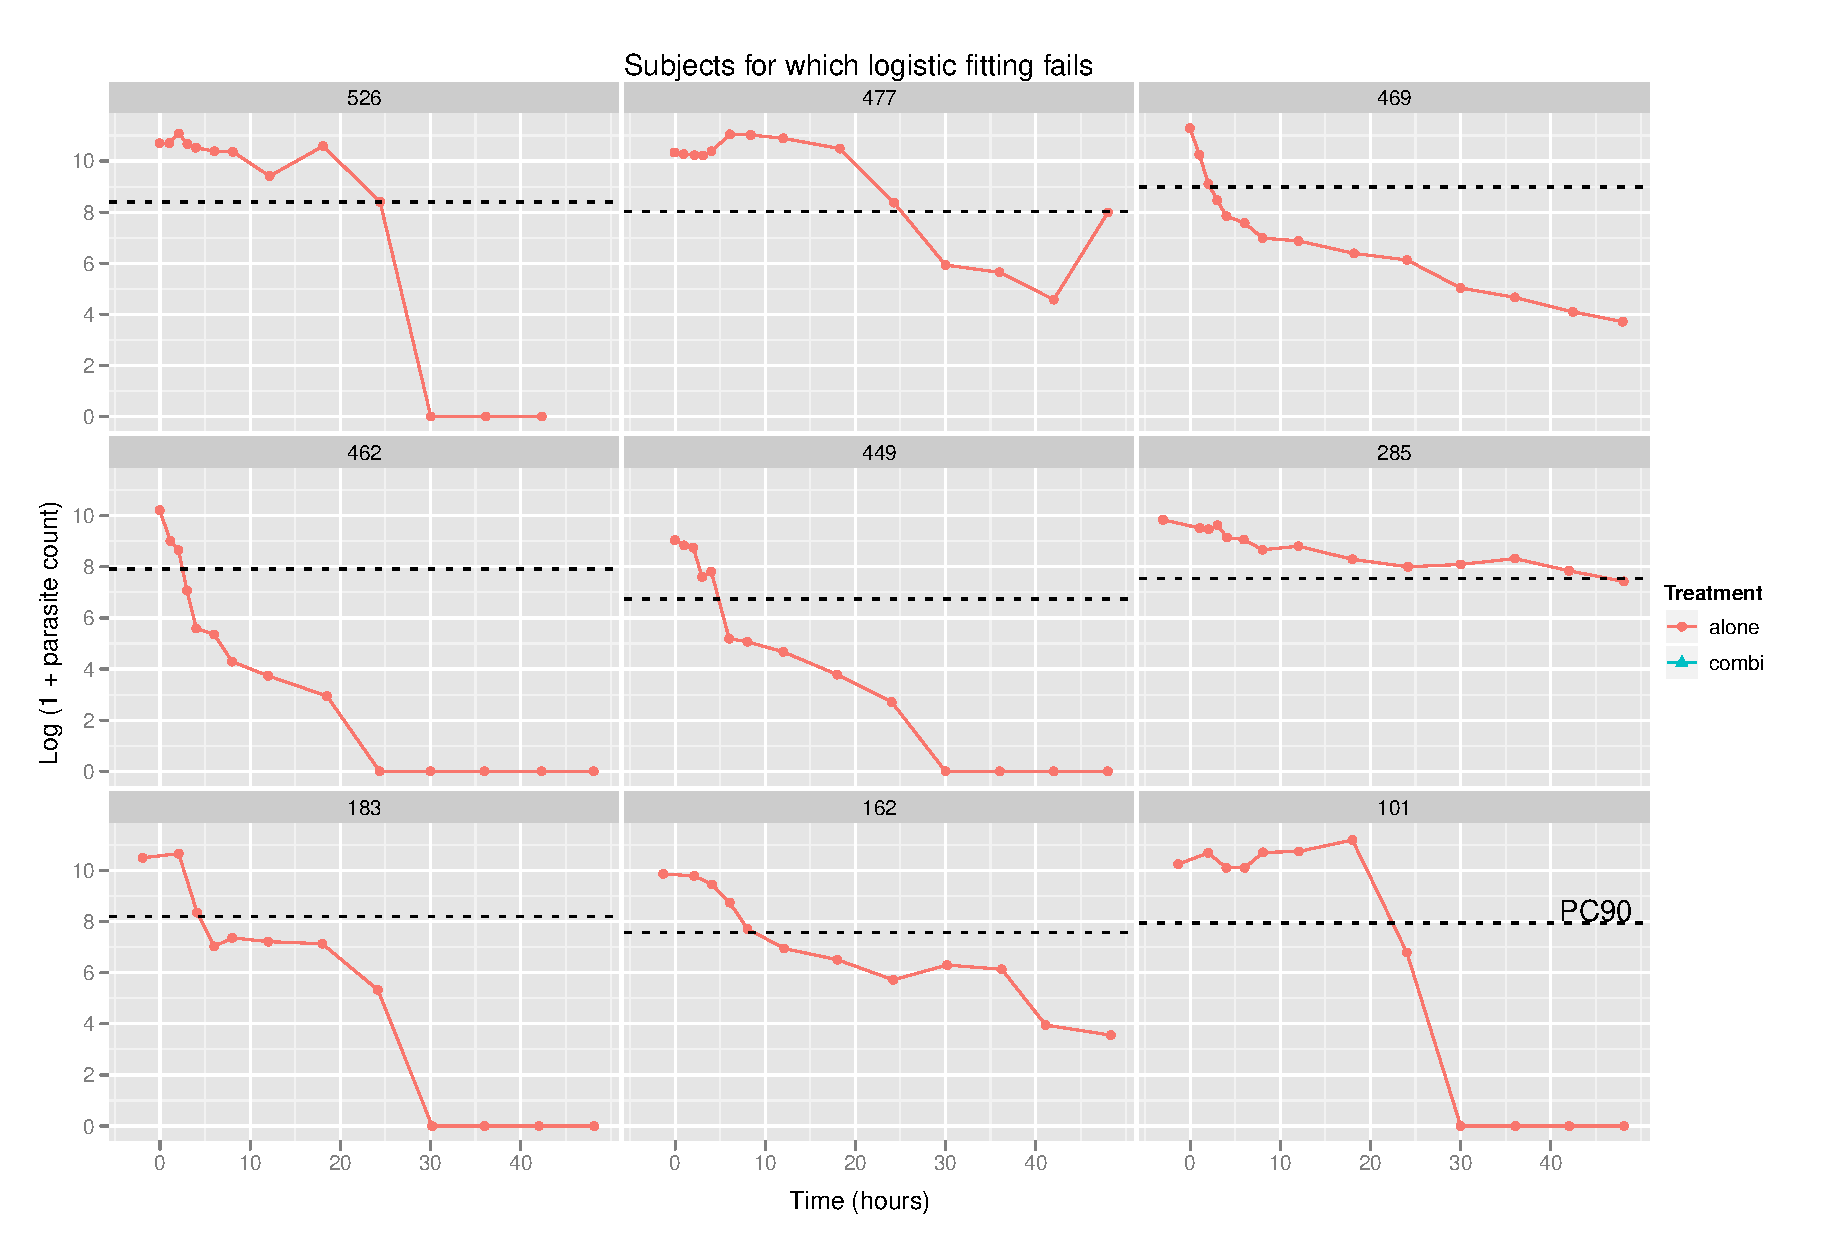
\includegraphics[width=150mm]{failures.eps} 
\caption{Subjects for which the logistic fitting fails}\label{failures}
\end{figure}

It is interesting to note that all subjects for which logistic fitting fails are in the single treatment group; $p=0.0039$ under the null hypothesis of equal probability of a subject being from the single or combined treatment group using a binomial model. This is evidence that the parasite counts for patients on the single treatment follow more varied trajectories during clearance compared to patients on the combined treatment whose clearance can consistently be described with a logistic or cubic model to a reasonable approximation.

In addition to parasite count profiles that simply do not conform to a logistic shape there were subjects where insufficient data in the region between the upper and lower asymptotes meant that logistic fitting was inappropriate. For example, subjects 526 and 101 in Figure \ref{failures}, where choice of different starting parameters for $\mu$ and $\beta$ would result in different logistic fits being obtained. One possible fit having a steep transition (large absolute $\beta$), whereby the data at the upper and lower levels is closely modelled. Another possible fit having a shallower transition (smaller $\beta$) that models the slope of a line passing through the ends of the run of points at the upper and lower levels and the point in the middle, but  has a less severe curvature such that the corners at the upper and lower levels are poorly modelled. In summary the fit is free to rotate about the single point between the upper and lower levels and thus cannot be suitably defined.

\subsection{Log-linear interpolation}
The datum immediately above the PC90 level is joined with a straight line to the datum immediately below the PC90 level in on a plot of $\log(1+P_{t})$ against time. The point where this line crosses the PC90 level determines $t$=PC90.

\section{Comparison of estimation methods}
Table \ref{PC90} shows a comparison of the PC90 estimates obtained by the 3 different methods utilised so far.
\begin{table}[p]
\centering
\caption{Comparison of PC90 estimated by 3 methods}\label{PC90}
\begin{tabular}{|cccc|rrr|}
\hline
Subject&Centre&&&PC90&PC90&PC90\\
ID&ID&Sex&Treatment&cubic&logistic&log-linear\\
\hline
54&Centre 1&Male&alone&3.82&4.14&3.85\\
80&Centre 1&Male&alone&27.62&28.50&27.32\\
96&Centre 1&Female&alone&21.18&22.95&19.76\\
98&Centre 1&Male&alone&34.50&33.51&36.30\\
101&Centre 1&Female&alone&23.20&-&22.45\\
140&Centre 1&Male&combi&9.47&10.16&9.47\\
150&Centre 1&Female&alone&22.52&23.12&21.75\\
162&Centre 1&Male&alone&10.54&-&8.84\\
176&Centre 1&Male&combi&5.32&5.66&5.05\\
182&Centre 1&Female&combi&3.98&4.29&3.65\\
183&Centre 1&Male&alone&4.55&17.21&4.35\\
185&Centre 1&Male&combi&7.59&8.13&8.10\\
187&Centre 1&Male&alone&1.81&3.05&1.53\\
197&Centre 1&Female&combi&8.38&8.35&8.40\\
203&Centre 1&Female&combi&10.48&10.30&9.69\\
218&Centre 1&Male&combi&23.48&23.92&22.77\\
224&Centre 1&Male&alone&28.86&30.26&30.01\\
262&Centre 1&Male&combi&9.40&9.85&9.40\\
264&Centre 1&Female&combi&0.37&1.43&0.85\\
280&Centre 1&Female&combi&8.76&9.72&9.04\\
285&Centre 1&Female&alone&47.74&-&46.52\\
288&Centre 1&Female&combi&12.86&12.38&9.38\\
294&Centre 1&Male&combi&8.86&8.68&7.73\\
295&Centre 1&Male&alone&5.02&4.98&4.83\\
449&Centre 2&Male&alone&4.45&-&4.82\\
453&Centre 2&Female&alone&19.66&23.08&21.97\\
462&Centre 2&Female&alone&2.11&-&2.49\\
469&Centre 2&Male&alone&3.01&-&2.21\\
477&Centre 2&Female&alone&24.03&-&25.08\\
490&Centre 2&Female&alone&28.73&29.94&31.63\\
500&Centre 2&Male&combi&19.36&19.66&17.15\\
502&Centre 2&Female&combi&15.33&16.33&14.77\\
504&Centre 2&Female&alone&5.07&6.64&5.00\\
505&Centre 2&Female&combi&8.26&9.02&8.75\\
509&Centre 2&Male&alone&20.59&18.63&11.59\\
511&Centre 2&Male&combi&10.00&10.91&9.51\\
519&Centre 2&Male&combi&15.63&16.08&14.68\\
521&Centre 2&Female&alone&22.14&23.38&21.64\\
523&Centre 2&Female&combi&5.82&5.97&5.84\\
525&Centre 2&Female&combi&6.15&6.17&6.23\\
526&Centre 2&Female&alone&23.48&-&24.42\\
530&Centre 2&Male&alone&29.10&29.28&28.09\\
532&Centre 2&Male&combi&9.16&9.21&8.08\\
\hline
\end{tabular}
\end{table}

\subsection{Graphical comparison}
Figure \ref{pc90-agree} shows 8 examples of subjects where estimation by the 3 different methods shows good agreement. It seems likely that the differences between these estimates are of a comparable scale to experimental error. It can be seen that the 3 methods give close agreement when the data can be closely modelled by cubic or logistic fitting and when the gradient of the log-linear interpolation is similar to the regression models in the region around PC90. 
\begin{figure}[h]
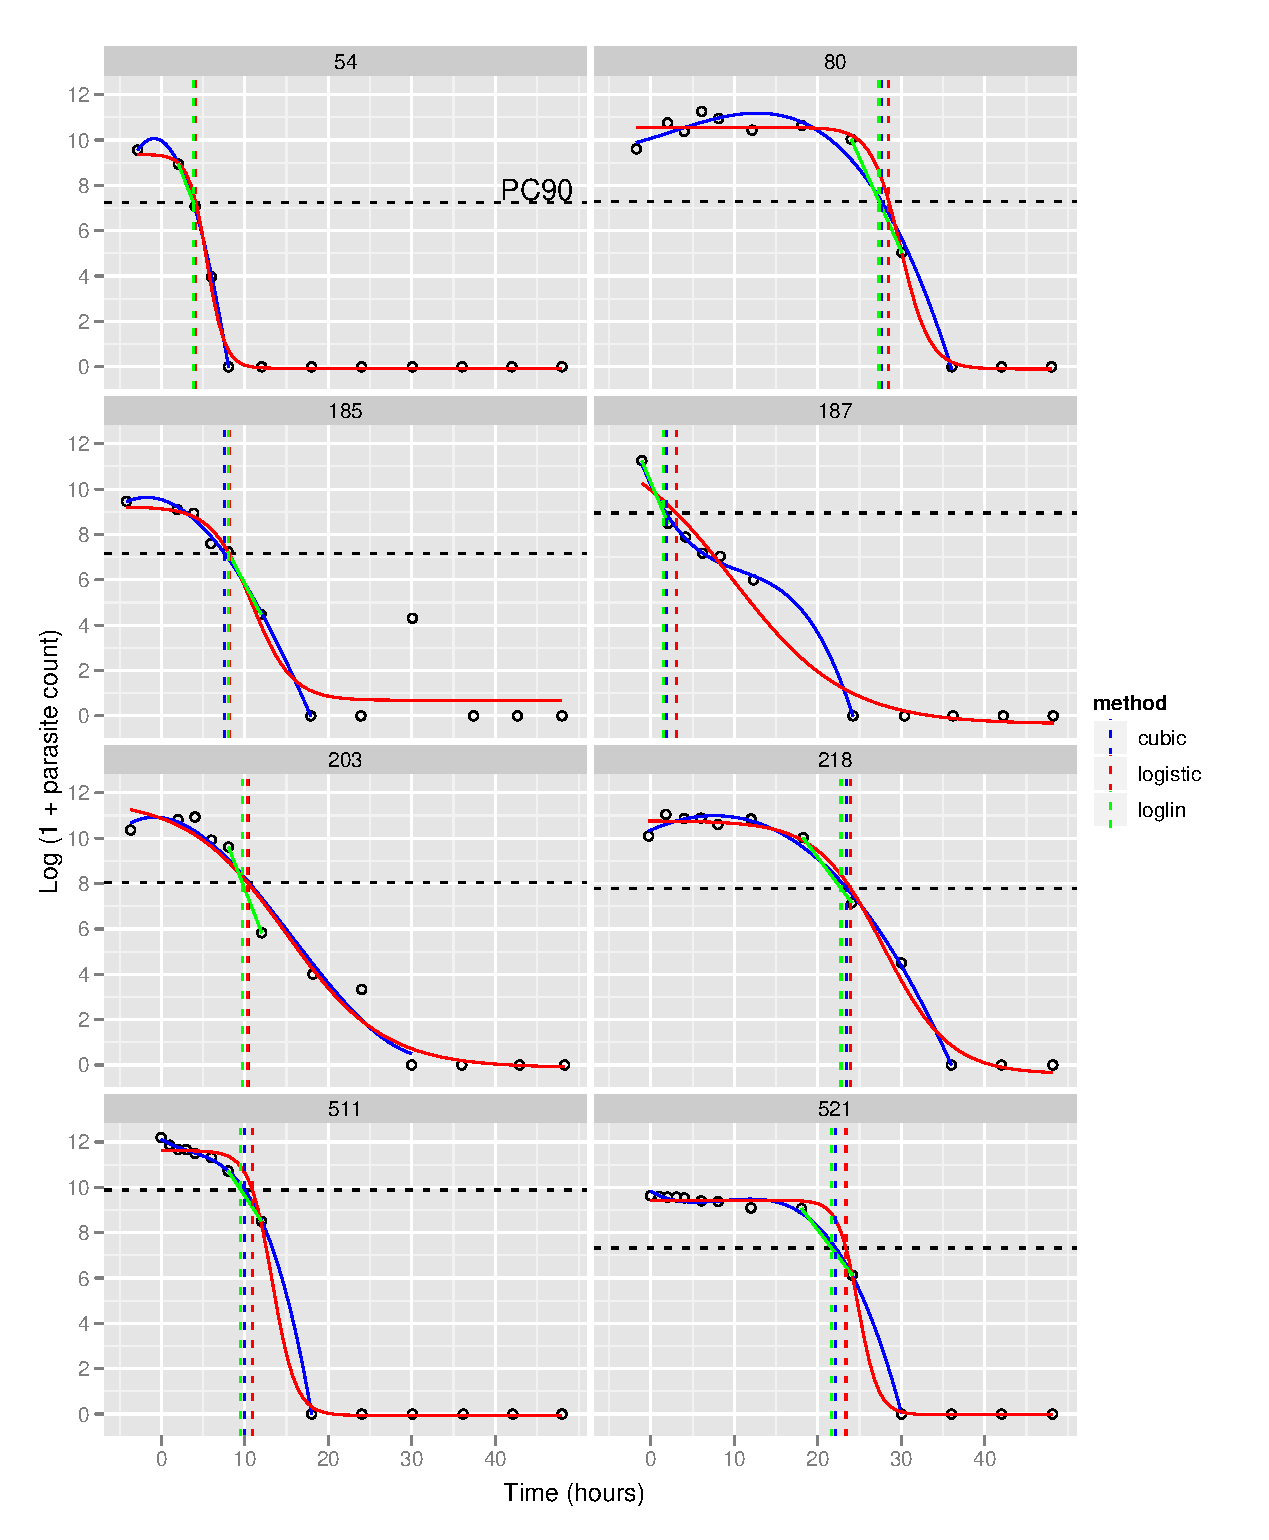
\includegraphics[width=150mm]{pc90-agree.eps} 
\caption{Subjects with little difference in PC90 estimated by 3 methods}
\label{pc90-agree}
\end{figure}

Figure \ref{pc90-bad} shows examples of subjects where estimation by the 3 different methods has resulted in notable differences between PC90 estimates. These differences appear to arise when:
\begin{enumerate}
\item The drop in parasite count is slow or stationary around the PC90 level e.g. subjects 98, 183, 453 and 509. In these cases the regression lines and interpolation may cross the PC90 level at markedly different times. In subject 183 this has given a difference in PC90 between the logistic and other two methods of over 10 hours.
\item There is ``unusual'' data near the PC90 level e.g. subjects 490 and 500 where recorded counts, seemingly off the prevailing trend, have influenced the interpolated estimate.
\end{enumerate}
\begin{figure}[h]
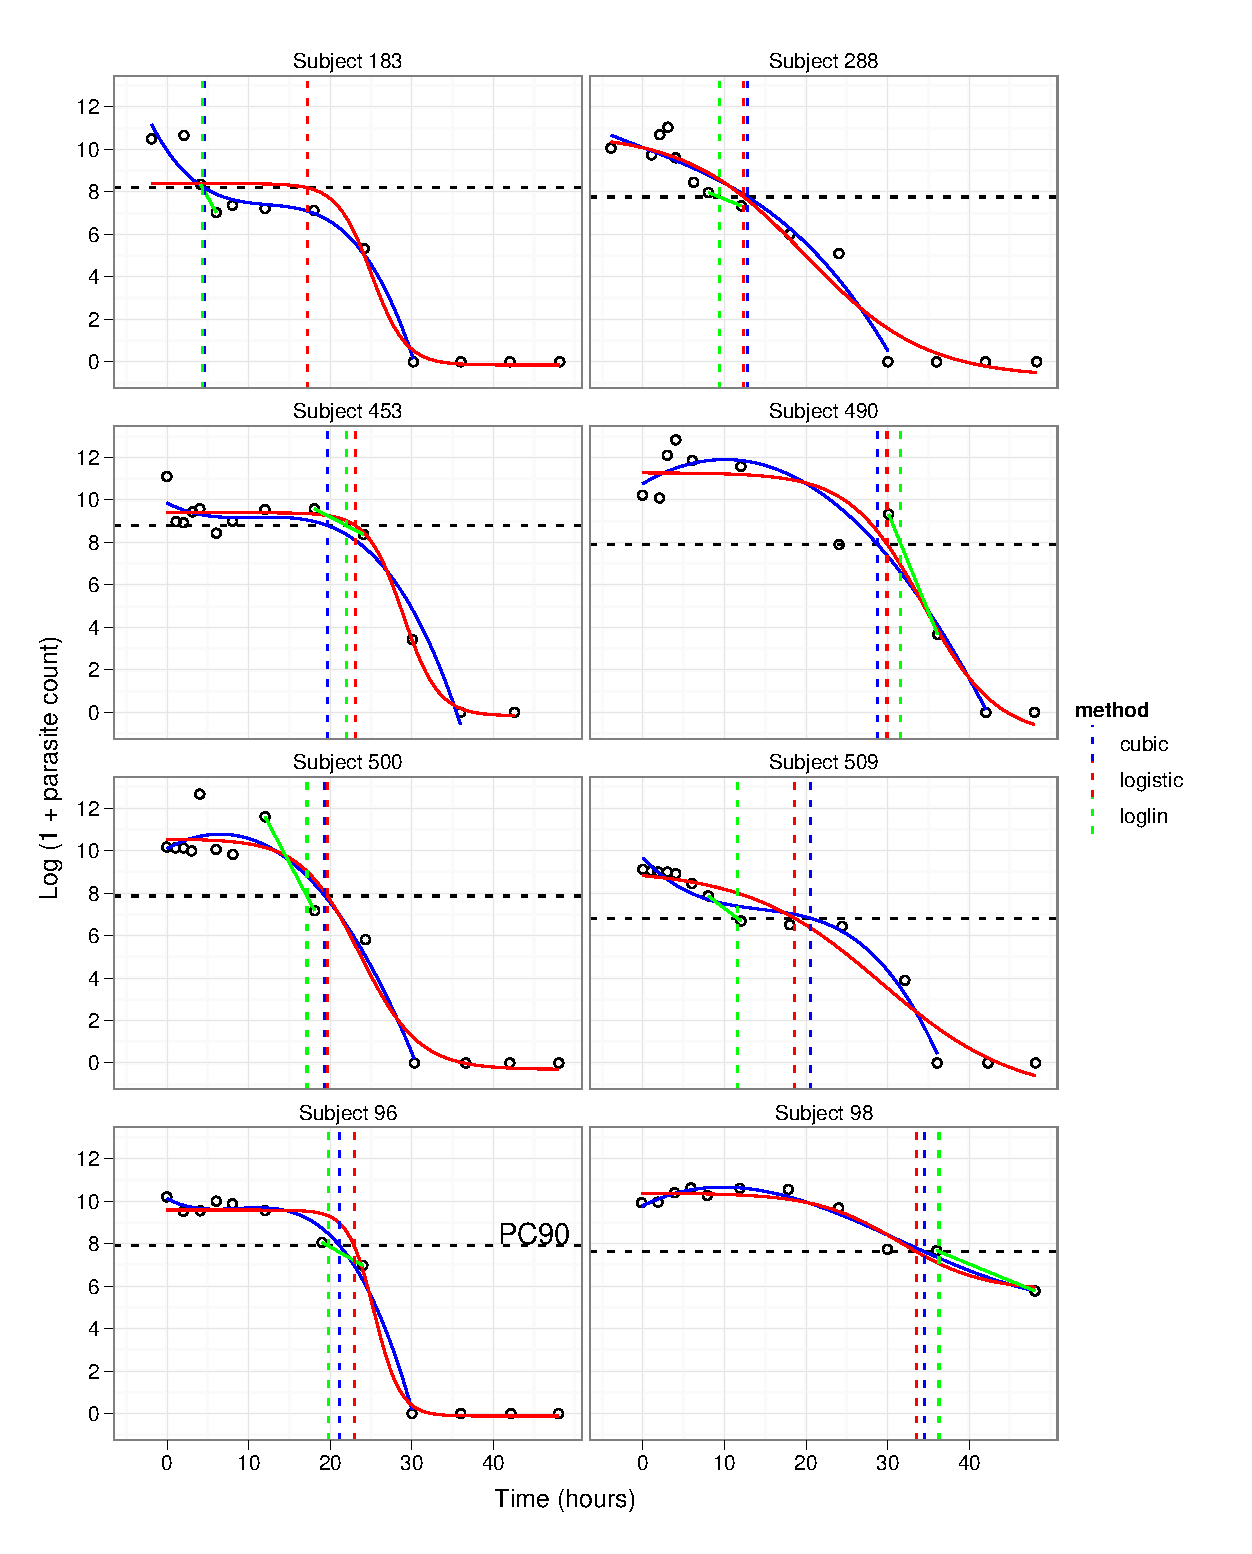
\includegraphics[width=150mm]{pc90-bad.eps} 
\caption{Subjects with notable difference in PC90 estimated by 3 methods}
\label{pc90-bad}
\end{figure}
Figure \ref{pc90-nofit} shows the cubic and log-linear interpolated estimates for subjects where logistic fitting was inappropriate.
\begin{figure}[hp]
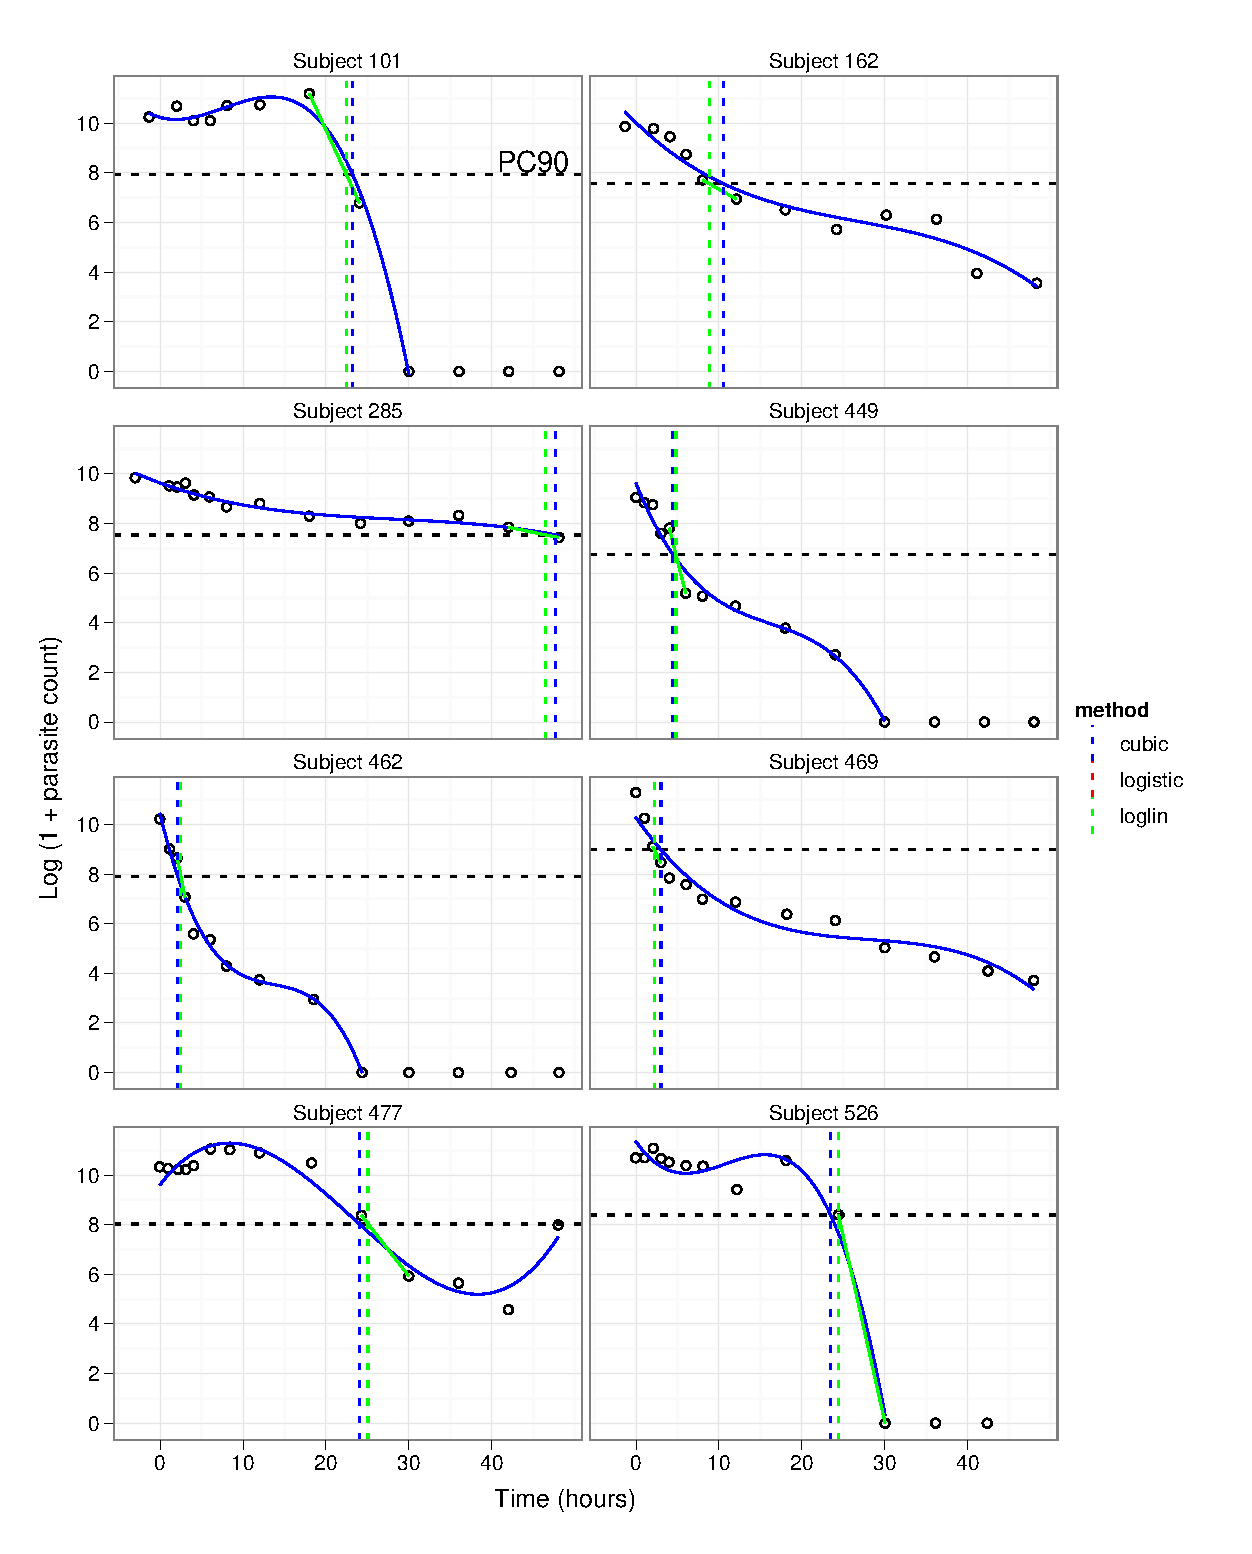
\includegraphics[width=150mm]{pc90-nofit.eps} 
\caption{PC90 estimation for subjects where logistic fitting was inappropriate}
\label{pc90-nofit}
\end{figure}
It can be seen that the two methods in these cases appear to produce very similar estimates.

\subsubsection*{Between and within subjects comparisons}
Figure \ref{methodsbysubject} shows the distribution of PC90 estimates between and within subjects. This is to give us an idea of what should be used as an error term in any modelling of the effect of the factors on PC90. The two ways of showing the distribution of PC90 estimates are:
\begin{description}
\item[Between subjects] - shows the distributions of residuals of PC90 values from the stratum mean i.e. the distribution of PC90 estimates about the mean at each unique centre-sex-treatment combination to which each subject belongs. In this way the distribution of the between-subjects ``error'' is shown.
\item[Within subjects] removes the effect of correlation between estimates made on the same subject by showing the distribution of the residuals of the PC90 estimate from the subject mean. In this way the distribution of within-subjects ``error'' is shown.
\end{description}
\begin{figure}[ht]
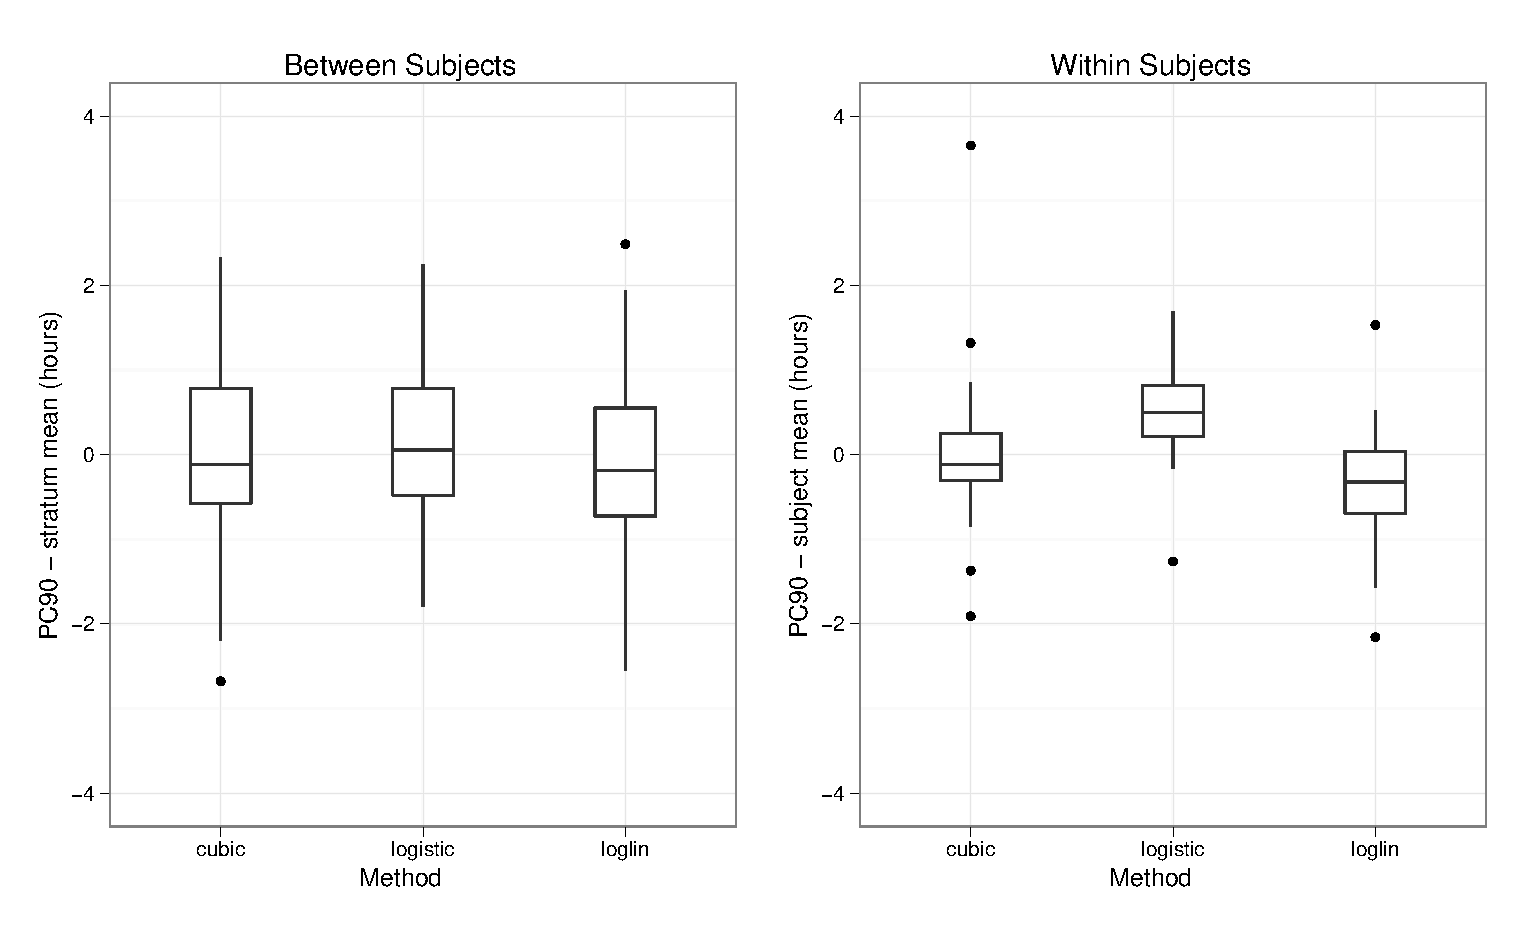
\includegraphics[width=150mm]{methodsbysubject.eps} 
\caption{Comparison of PC90 estimates between and within subjects}
\label{methodsbysubject}
\end{figure}

It can be seen that the choice of method only seems to have a significant effect within subjects with the logistic method appearing to give estimates higher than average and the log-linear interpolation method slightly lower. This suggests that variance between methods is only significant within subjects. It also shows that in any modelling of PC90 that the error between subjects is larger than that due to choice of PC90 estimation method.
% \subsubsection{Interaction of estimation method with experimental factors}
% Figures \ref{methodsbycentre}, \ref{methodsbysex} and \ref{methodsbytreatment} show the between and within subject PC90 estimates split by experimental factors centre, sex and treatment respectively:
% \begin{itemize}
% \item There does not seem to be any significant difference in the relationship between the 3 methods between centres.
% \item Sex does not appear to alter the relationship between the 3 methods.
% \item The three methods perhaps show closer agreement on the combined treatment.
% \end{itemize}
% In summary it does not seem that there are any significant interactions between the experimental factors and the estimates produced by the 3 methods.
% \begin{figure}[p]
% \includegraphics[width=150mm]{methodsbycentre.eps} 
% \caption{Comparison of PC90 estimates by centre}
% \label{methodsbycentre}
% \end{figure}
% \begin{figure}[p]
% \includegraphics[width=150mm]{methodsbysex.eps} 
% \caption{Comparison of PC90 estimates by sex}
% \label{methodsbysex}
% \end{figure}
% \begin{figure}[p]
% \includegraphics[width=150mm]{methodsbytreatment.eps} 
% \caption{Comparison of PC90 estimates by treatment}
% \label{methodsbytreatment}
% \end{figure}
\clearpage
\subsection{Statistical comparison}
%If we perform 2-way ANOVA between the 3 PC90 estimates by subject and method i.e.
%$$\mathrm{PC}90_{ij}=subject_{i}+method_{j}+\epsilon_{ij}\quad\quad\epsilon\sim N(0,\sigma^{2})$$ 
%we obtain the residuals shown in Figure \ref{pc90resid}.
%It can be seen that there are several outlying data points at up to $4\sigma$ and almost $8\sigma$. These correspond to subjects 183 and 509 for whom we obtained very different PC90 estimates by the 3 methods. As can be seen in Figure \ref{pc90-bad}, this is due to the parasite count being fairly constant around the PC90 level for these subjects.
%
%If we repeat the ANOVA analysis with subjects 183 and 509 removed, we obtain the residuals shown in Figure \ref{pc90resid-sub}.
%It can be seen that the residuals are approximately normally distributed with no obvious structure except for perhaps a smaller variance at smaller PC90 times. The results of the ANOVA analysis are shown in Table \ref{pc90aov}.
%\begin{table}[h]
%\centering
%\caption{ANOVA comparison of PC90 estimated by 3 methods}\label{pc90aov}
%\begin{tabular}{l|rrrrr}
%Source&Sum Sq.&df&Mean Sq.&$F$&P($>F$)\\
%\hline
%Subject&12023.7&40&300.6&558.8&$<1\times 10^{-15}$\\
%Method&12.1&2&6.0&11.2&$5.7\times 10^{-5}$\\
%Residual&38.7&72&0.54&&\\
%\hline
%Total&12074.5&114&&&
%\end{tabular}
%\end{table}
To perform a statistical comparison between the PC90 estimation methods we want to test the null hypothesis that the difference between PC90 estimated by each method is zero. In order to do this we need to look at the distribution of the differences between PC90 estimates and accordingly choose an appropriate statistical test.

\subsubsection*{Distributions of differences}
\begin{description}
\item[Cubic and logistic methods] - The distribution of the difference between PC90 estimated by the cubic and logistic methods is shown in Figure \ref{cub-log}. Apart from one outlying datum it can be seen that the differences are approximately normally distributed. The outlying value corresponds to subject 183, which we can see in Figure \ref{pc90-bad} gives a very different estimate by the two methods due to the parasite count being fairly constant around the PC90 level.
\item[Cubic and log-linear interpolation methods] - The distribution of the difference between PC90 estimated by the cubic and log-linear interpolation methods is shown in Figure \ref{cub-loglin}.
Again the distribution is approximately normally distributed apart from a single outlying value corresponding to subject 509. We can see in Figure \ref{pc90-bad} that again this corresponds to estimates made in a region where the parasite count is flat.
\item[Logistic and log-linear interpolation methods] - The distribution of the difference between PC90 estimated by the logistic and log-linear interpolation methods is shown in Figure \ref{log-loglin}. The two outlying values correspond to subjects 183 and 509 again.
\end{description}
As the distributions of differences are all approximately normally distributed, apart from a few anomalous estimates as described, we can used paired-sample $t$ tests to test our null hypothesis.
\begin{figure}[p]
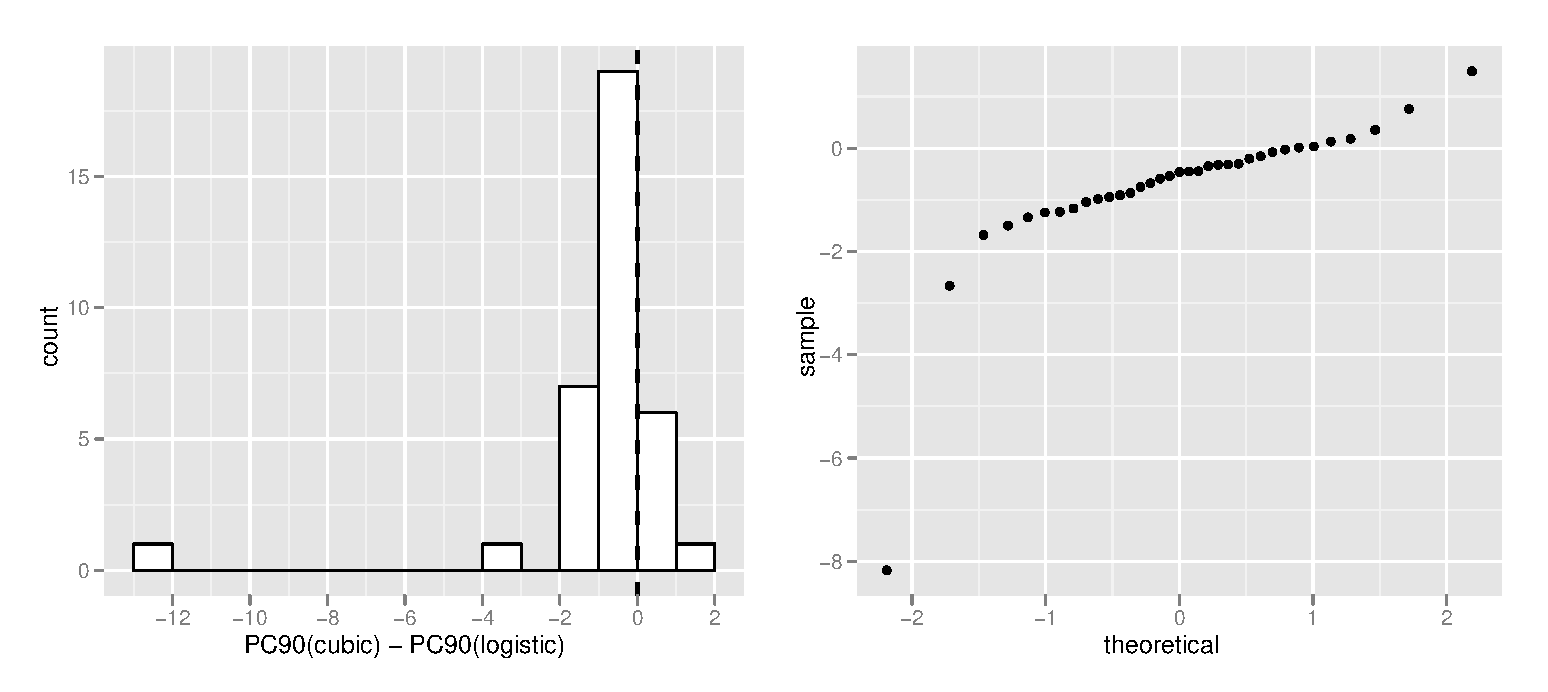
\includegraphics[width=150mm]{cub-log.eps} 
\caption{Distribution of the difference between PC90 estimated by the cubic and logistic methods}
\label{cub-log}
\end{figure}
\begin{figure}[p]
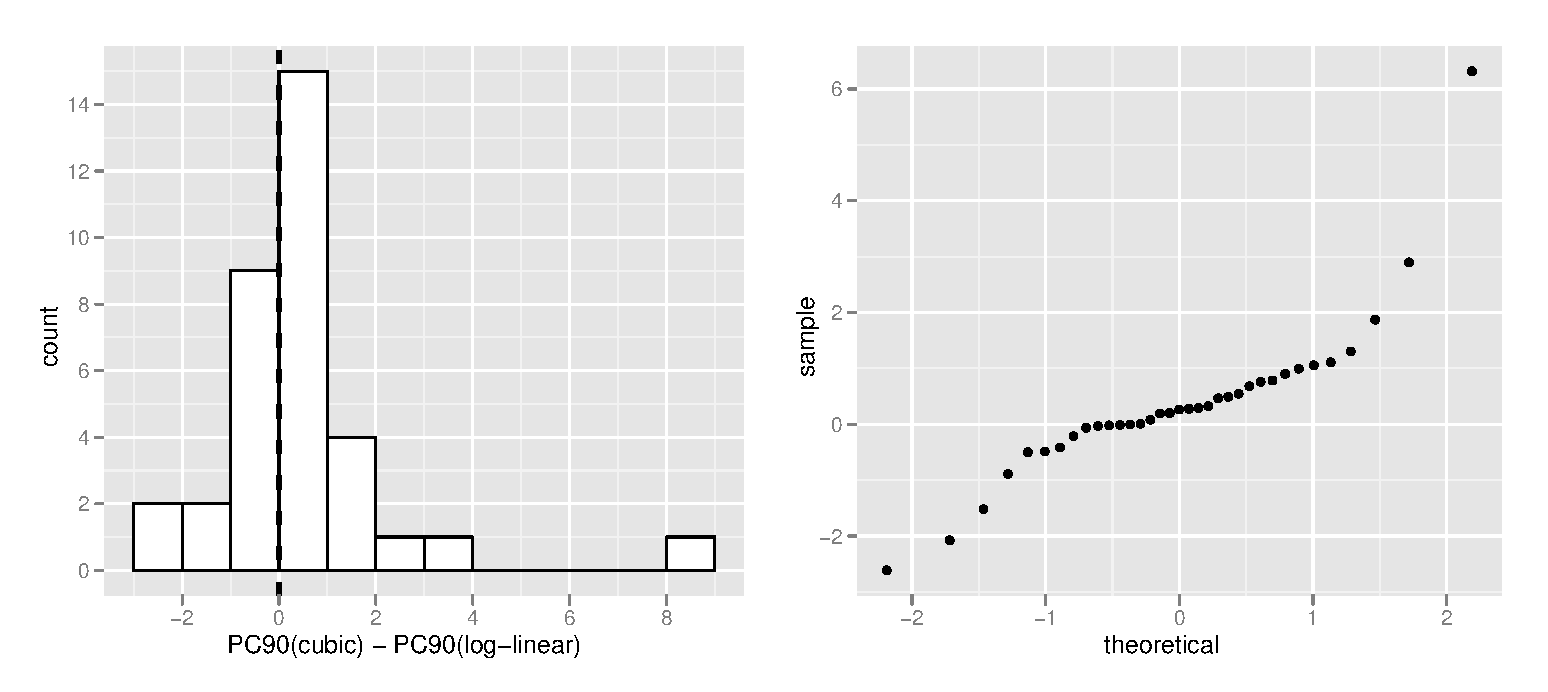
\includegraphics[width=150mm]{cub-loglin.eps} 
\caption{Distribution of the difference between PC90 estimated by the cubic and log-linear interpolation methods}
\label{cub-loglin}
\end{figure}
\begin{figure}[p]
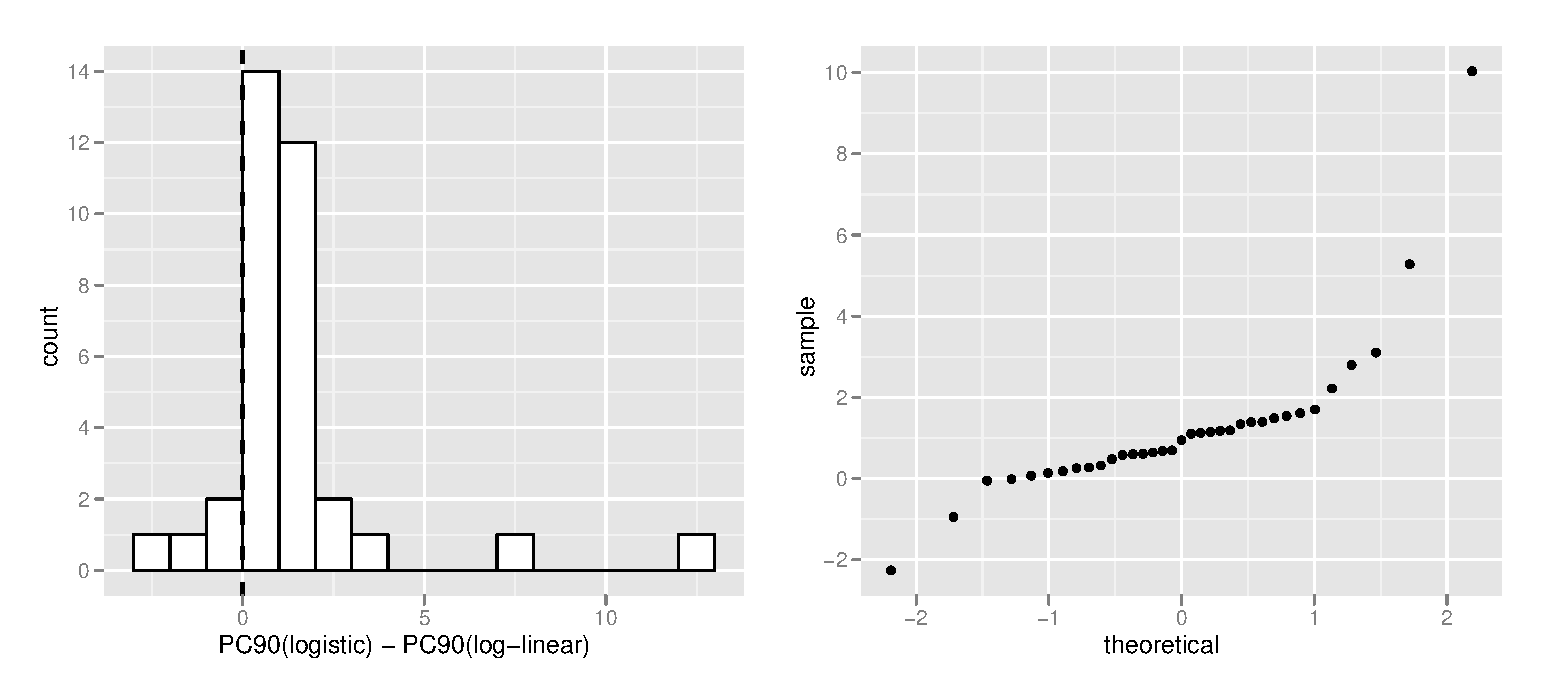
\includegraphics[width=150mm]{log-loglin.eps} 
\caption{Distribution of the difference between PC90 estimated by the logistic and log-linear interpolation methods}
\label{log-loglin}
\end{figure}

\subsubsection*{Paired $t$ tests}
\begin{description}
\item[Cubic and logistic methods] - If we perform a paired $t$ test between PC90 estimated by the cubic and logistic methods, excluding subject 183, we find good evidence to reject the hypothesis that the two methods result in the same PC90 estimate ($P<0.005$). On average the logistic method gives PC90 32 minutes longer than the cubic method with a 95\% confidence interval of (13, 51) minutes, bearing in mind this is only based on a comparison of the subset of 35 subjects for which a logistic fit was possible out of the total of 43.
\item[Cubic and log-linear interpolation methods] - A paired $t$ test excluding subject 509 gives no evidence to reject the hypothesis that the cubic and log-linear interpolation methods give the same PC90 estimates.
\item[Logistic and log-linear interpolation methods] - A paired $t$ test excluding subjects 183 and 509 gives good evidence to reject the hypothesis that the logistic and log-linear methods produce the same PC90 estimates ($P<0.0005$). On average the logistic method produces PC90 estimates 49 minutes longer than the log-linear interpolation method with a 95\% confidence interval of (25, 73) minutes.
\end{description}
\subsubsection*{ANOVA}
The results of 4-way ANOVA on the 121 PC90 estimates (3 estimates for each of 43 subjects, minus 8 where no logistic estimate could be made), classified by estimation method, centre, sex and treatment with all interactions are shown in Table \ref{pc90aov}. A square-root transformation of the P90 dependent variable was used for variance stabilisation; it will be shown in chapter \ref{ch:analysis} that this is appropriate for this data. Only the results for the effect of the PC90 method used and its 2-way interactions are shown here so as not to pre-empt the analysis of chapter \ref{ch:analysis}. 3-way and higher interactions were all non-significant.
%> summary(PC90methods.within.aov)
%                            Df  Sum Sq Mean Sq F value    Pr(>F)    
%Method                       2   0.438   0.219  0.1345 0.8742919    
%Centre                       1   1.356   1.356  0.8319 0.3639784    
%Sex                          1   0.226   0.226  0.1385 0.7106024    
%Treatment                    1  27.955  27.955 17.1533 7.366e-05 ***
%Method:Centre                2   0.981   0.490  0.3008 0.7408770    
%Method:Sex                   2   1.973   0.987  0.6054 0.5479050    
%Centre:Sex                   1   1.152   1.152  0.7072 0.4024495    
%Method:Treatment             2   0.320   0.160  0.0980 0.9067164    
%Centre:Treatment             1   1.648   1.648  1.0113 0.3170836    
%Sex:Treatment                1  20.927  20.927 12.8409 0.0005326 ***
%Method:Centre:Sex            2   0.215   0.107  0.0659 0.9362209    
%Method:Centre:Treatment      2   0.843   0.421  0.2585 0.7727248    
%Method:Sex:Treatment         2   1.371   0.685  0.4206 0.6578573    
%Centre:Sex:Treatment         1   2.040   2.040  1.2520 0.2659387    
%Method:Centre:Sex:Treatment  2   0.056   0.028  0.0173 0.9828618    
%Residuals                   97 158.081   1.630                   
\begin{table}[h]
\centering
\caption{ANOVA comparison of PC90 estimated by 3 methods}\label{pc90aov}
\begin{tabular}{l|rrrrr}
Source&Sum Sq.&df&Mean Sq.&$F$&P($>F$)\\
\hline
$Method$&0.438&2&0.219&0.135&$0.874$\\
$Method\times Centre$&0.981&2&0.490&0.301&$0.741$\\
$Method\times Sex$&1.973&2&0.987&0.605&0.548\\
$Method\times Treatment$&0.320&2&0.160&0.098&0.907\\
$\vdots$&$\vdots$&$\vdots$&$\vdots$&$\vdots$&$\vdots$\\
$All\ other\ terms$&57.8&15&3.85&&\\
$\vdots$&$\vdots$&$\vdots$&$\vdots$&&\\
$Residuals$&158.08&97&1.630&&\\
\hline
Total&219.58&120&&&
\end{tabular}
\end{table}

It can be seen that there is no evidence that the variance in PC90 between estimation methods is any larger than the variance between subjects in each centre-sex-treatment stratum. Therefore the difference between PC90 estimates is independent of other factors. If we fit a multilevel model such that our residual variance is partitioned into that between subjects and that within subjects (between methods) i.e.
\begin{eqnarray*}
\sqrt{\mathrm{PC}90}=\mathrm{main\ effects\ + interactions} + b_{l} + \epsilon_{lm}\\
b_{l}\sim N(0,\sigma_{b}^{2})\quad\quad\epsilon_{lm}\sim N(0,\sigma^{2})
\end{eqnarray*}
for subject $l$ and method $m$ then we find $\sigma_{b}^{2}=1.64$ (compare with mean-square residual in Table \ref{pc90aov}) and $\sigma^{2}=0.052$. This quantifies the relative magnitudes of the between and within subjects variance, as shown in Figure \ref{methodsbysubject} on page \pageref{methodsbysubject}, and shows that the ``error'' due to between-subject variations is larger than the error due to choice of method.

The full results of the relative effects of all factors can be found in chapter \ref{ch:analysis}. At this stage we are just concerned with the effect of choice of PC90 estimation method. In summary the $t$ tests show us that the difference between methods is significant within subjects for 2 out of the 3 comparisons. The ANOVA analysis shows that it is insignificant in comparison to the variation due to centre, sex and treatment.
\subsubsection*{Correlation of difference with magnitude}
We have deduced from the 4-way ANOVA with interactions that there is no interaction between the method chosen and the other factors that influences the PC90 estimation. The $t$ tests told us the average amount that the methods differ, if at all, and in which direction, but we should check if the difference between the methods is related to the size of the PC90 estimates. The difference in PC90 estimate between the methods is plotted against the mean estimate in Figure \ref{pc90est-cor}.
\begin{figure}[h]
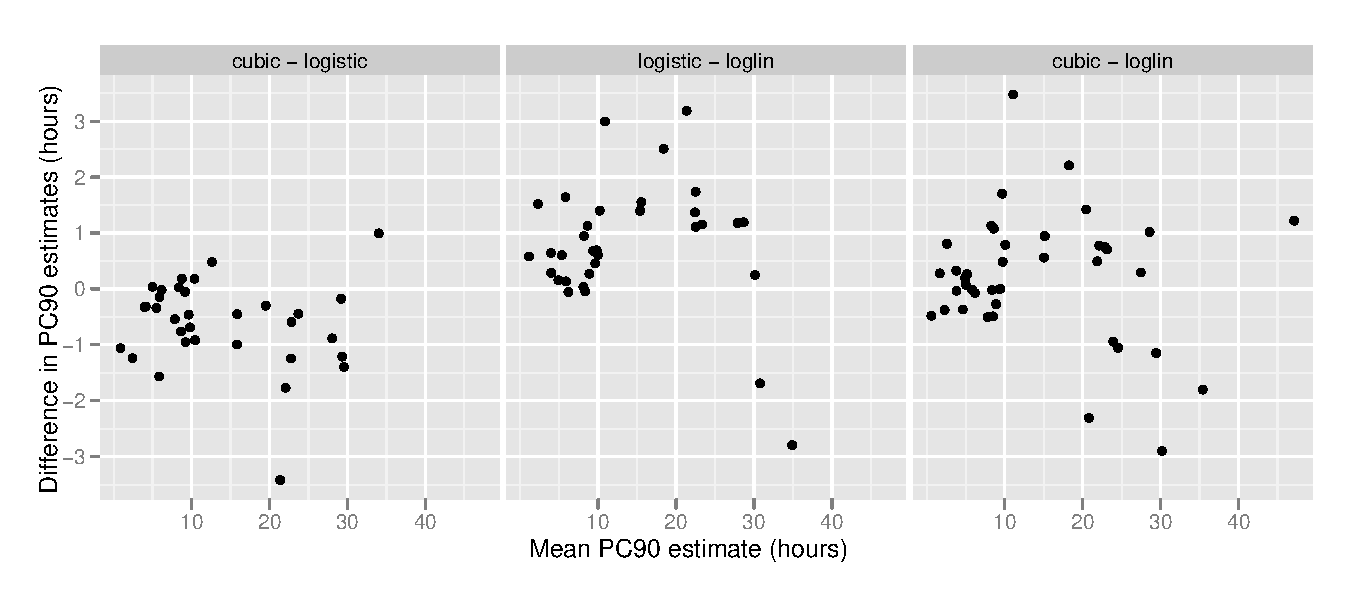
\includegraphics[width=150mm]{pc90est-cor.eps} 
\caption{Difference in PC90 estimates against mean PC90 estimate}
\label{pc90est-cor}
\end{figure}

There is no obvious correlation and Spearman rank tests do not give any evidence to reject the null hypothesis of 0 correlation. This means that we can expect the methods to give PC90 estimates that differ by the amounts given by the $t$ tests independent of the size of the PC90 estimate.
\section{Key Results}
The key results from this investigation into methods for derivation of parasite clearance times are:
\begin{itemize}
\item The log-transformed parasite count from pre-dose up to the first zero count can be modelled by cubic polynomial linear regression. The combined treatment data seems to be more closely modelled by the cubic fit than the single treatment data.
\item The log-transformed parasite count can be modelled by a logistic non-linear model for 35 out of the 43 subjects. For the other 8 subjects it was found that a logistic model is inappropriate and ambiguous at best.
\item The subjects that could not be modelled by the logistic method were all from the single treatment group ($P<0.005$), indicating that patients on the single treatment show a different response to patients on the combined treatment.
\item A log-linear interpolation gives a simple alternative to regression methods for estimating PC90.
\item The cubic linear model and log-linear interpolation methods give statistically the same PC90 estimate averaged over all subjects: no evidence to reject null hypothesis of zero mean difference between PC90 estimates.
\item The logistic non-linear model produces PC90 estimates 32 minutes longer than the cubic method 
with a 95\% confidence interval of (13, 51) minutes.
\item The logistic method produces PC90 estimates 49 minutes longer than the log-linear interpolation method with a 95\% confidence interval of (25, 73) minutes.
\item The variance in PC90 between methods is smaller than that between subjects. Hence, choice of estimation method is not crucial and any weighting based on an error derived from between-method variation would be swamped by between-subject variation.
\item The difference in PC90 due to estimation method is independent of sex, centre and treatment and magnitude of PC90. 
\end{itemize}
\subsection{Choice of PC90 estimation method}
The key advantages and disadvantages of each method are shown in Table \ref{pc90compare}.
\begin{table}[h]
\centering
\caption{Comparison of PC90 estimation methods}\label{pc90compare}
\begin{tabular}{|m{1.4in}|m{2.0in}|m{2.0in}|}
\hline
Method&Advantages&Disadvantages\\\hline
Cubic polynomial\newline linear regression&
\begin{list}{\labelitemi}{\leftmargin=1em}
\item Simple to fit.
\item Fits all subjects.
\item Fairly robust to erratic variation in PC90 region.
\end{list}&
\begin{list}{\labelitemi}{\leftmargin=1em}
\item Only models data up to first zero count.
\end{list}
\\\hline
Logistic non-linear\newline regression&
\begin{list}{\labelitemi}{\leftmargin=1em}

\item Models data over whole time period.
\item Fairly robust to erratic variation in PC90 region.
\end{list}&
\begin{list}{\labelitemi}{\leftmargin=1em}
\item Fitting procedure is complicated requiring choice of initial parameters.
\item Does not find a suitable fit for all subjects.
\end{list}
\\\hline
Log-linear\newline interpolation&
\begin{list}{\labelitemi}{\leftmargin=1em}
\item Simple to fit.
\item Fits all subjects.
\end{list}&
\begin{list}{\labelitemi}{\leftmargin=1em}
\item Only models PC90 region.
\item Sensitive to variation in PC90 region.
\end{list}
\\\hline
\end{tabular}
\end{table}

It appears that, for the purpose of PC90 estimation, there is little to choose between the cubic and log-linear interpolation methods. The cubic method will be more robust to the occurrence of spurious data in the PC90 region, although for the subjects studied here this does not seem to have greatly influenced estimates using log-linear interpolation. In fact if we look at subjects 500 and 509 in Figure \ref{pc90-bad} we see that although the log-linear interpolation differs from the other two estimates it has actually detected the time at which the primary endpoint is reached most accurately i.e. has produced an estimate closest to the first actual datum below the PC90 level.

There does not appear to be a compelling reason to use the logistic method. Although it perhaps models the behaviour at the upper and lower asymptotes better than the cubic method, it is not these regions that are of interest for estimating PC90. The fact that it is difficult to fit the logistic model and that it cannot fit almost 20\% of subjects also adds weight to using other methods.

The logistic model investigated here is the same one used by Wootton \textit{et al}.\cite{wootton}. However, they specify that the best model fit was chosen by two independent statisticians based on criteria such as the effect of outliers on the model fit and fit of the model in the baseline region. This is in contrast to the objective fit obtained here by use of computational fitting routines, the only input being starting parameters to help the routine arrive at a solution. Wootton \textit{et al}. discarded the data when no suitable logistic fit could be found. If these subjects were more likely to be from one treatment group, as we found here, this would unbalance the experiment.

Carmello \textit{et al}.\cite{carmello} use the log-linear interpolation method for estimating PC90. The only similar study employing polynomial regression found was that of de Vries \textit{et al.}\cite{vries} who experiment with use of a quadratic in time to model the log parasite count, but ultimately chose a model without a quadratic term.

In summary it would seem that the log-linear interpolation method seems the most suitable for estimating PC90, in terms of its simplicity and that it appears to consistently estimate sensible PC90 values as determined by graphical inspection. Perhaps estimates using the cubic method could also be easily computed and where the two methods disagree by a large amount e.g. greater than $3\sigma$ as for subject 509 here (Figures \ref{pc90-bad} and \ref{cub-loglin}), then these subjects could be flagged for closer inspection.

%\subsection{Other possible methods}
%One method of PC90 estimation that could combine the advantages of cubic and log-linear interpolation is 
\chapter{Analysis of Parasite Clearance Times}\label{ch:analysis}
The derived PC90 values using the log-linear interpolation method are shown in Table \ref{derivedPC90}.
\begin{table}[h]
\centering
\caption{Derived PC90 values in hours}\label{derivedPC90}
\begin{tabular}{|cc|c|c|}
\hline
&&\multicolumn{2}{c|}{Treatment}\\
&&alone&combined\\\hline
\multirow{2}{*}{Centre 1}&Male&$\begin{array}{c}3.85,\ 27.32,\ 36.30,\  8.84,\\4.35,\  1.53,\ 30.01,\  4.83\end{array}$&$\begin{array}{c}9.47,\  5.05,\  8.10,\\22.77,\  9.40,\  7.73\end{array}$\\\cline{2-4}
&Female&$\begin{array}{c}19.76,\ 22.45,\\21.75,\ 46.52\end{array}$&$\begin{array}{c}3.65,\ 8.40 ,\ 9.69,\\0.85,\ 9.04,\ 9.38\end{array}$\\\hline
\multirow{2}{*}{Centre 2}&Male&$\begin{array}{c}4.82,\ 2.21,\\11.59,\ 28.09\end{array}$&$\begin{array}{c}17.15,\ 9.51,\\14.68,\ 8.08\end{array}$\\\cline{2-4}
&Female&$\begin{array}{c}21.97,\ 2.49,\ 25.08,\ 31.63,\\5.00,\ 21.64,\ 24.42\end{array}$&$\begin{array}{c}14.77,\  8.75,\\5.84,\ 6.23\end{array}$\\\hline
\end{tabular}
\end{table}
Summary statistics are shown in Table \ref{summaryPC90}.
\begin{table}
\centering
\caption{Summary statistics for PC90 in hours}\label{summaryPC90}
\begin{tabular}{|l|ccc|ccc|}
\hline
&\multicolumn{6}{c|}{Treatment}\\
&\multicolumn{3}{c|}{alone}&\multicolumn{3}{c|}{combined}\\
&mean&median&sd&mean&median&sd\\
\hline
Centre 1	& 19.0 & 20.8 & 14.5 & 8.6  &  8.7  &  5.2 \\
Centre 2	& 16.3  & 21.6 &  11.2 & 10.6  &  9.1  &  4.3 \\
\hline
Male		& 13.6  &  6.8 & 12.9 & 11.2  &  9.4 &   5.4 \\
Female	& 22.1  & 22.0 &  11.8 & 7.7  &  8.6  &  3.8  \\
\hline
All		& 17.7  & 21.6 &  12.8 & 9.4  &  8.9  &  4.9  \\
\hline 
\end{tabular}
\end{table}

It can be seen that PC90 is generally shorter for subjects on the single drug (``alone'') treatment than those on the combined drug treatment across both centres. However, male patients have a higher median PC90 on the combined treatment. Standard deviations are notably higher for the single treatment. There do not seem to be any clear differences between centres. Females have longer PC90 times than males on the alone treatment with the opposite trend on the combined treatment.

\section{Graphical comparison}
The PC90 data from Table \ref{derivedPC90} are plotted by factors centre, sex and treatment in Figure \ref{pc90boxes}, summarized in two ways. Firstly, by the median and upper and lower quartiles. Secondly, the mean is shown with 95\% confidence intervals from the $t$ distribution defined by the standard error of the data%\footnote{The $t$ distribution confidence intervals are calculated using the \texttt{smean.cl.normal} \emph{R} functions from the Hmisc library \cite{Hmisc}}
. These confidence intervals for the mean are relevant for parametric tests based on the normal distribution such as ANOVA and give an indication of differences that may be significant.
\begin{figure}[h]
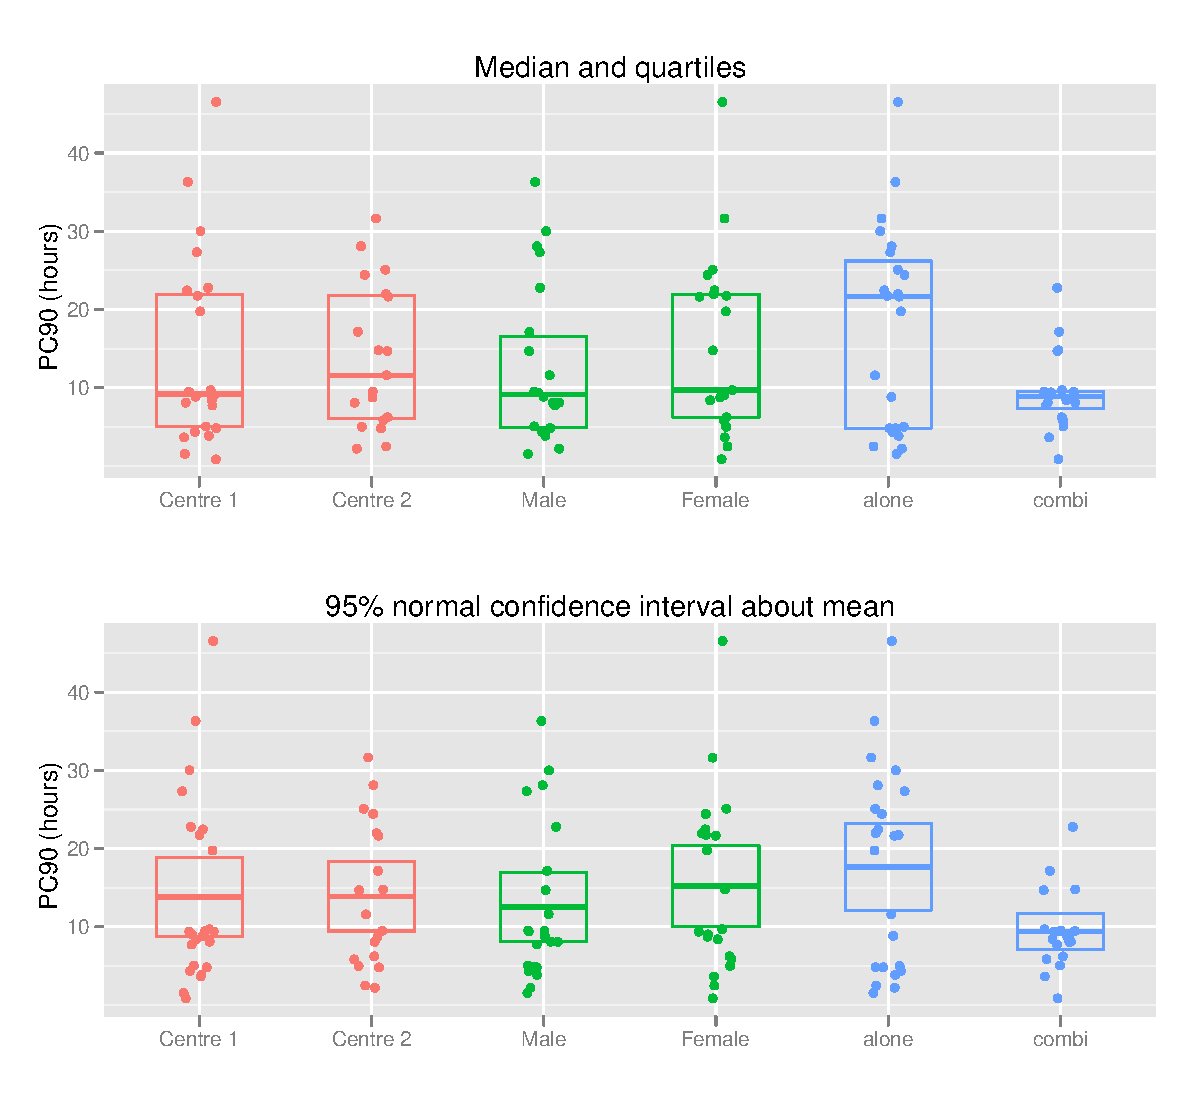
\includegraphics[width=150mm]{pc90boxes.eps} 
\caption{Comparison of PC90 by experimental factors with box plots showing medians and quartiles (top) and means with $t$ distribution 95\% confidence intervals (bottom)}
\label{pc90boxes}
\end{figure}

It can be seen in Figure \ref{pc90boxes} that there doesn't seem to be any notable difference in clearance times between centres. Female subjects seem to have a larger variance in clearance times and perhaps a slightly longer clearance time on average. The difference in clearance times due to the treatment chosen seems to have the largest influence with a larger spread in clearance times for subjects on the ``alone'' single-drug treatment with a potentially significant decrease in mean clearance time for the subjects on the combined-drug treatment.

An additional observation is that the distributions seem bimodal in the cases of the centre 1, female and alone treatment subjects. Looking at the plots of PC90 derivation in the previous chapter (Figures \ref{pc90-agree} to \ref{pc90-nofit}), it is not clear why this is. There does not seem to be an indication that this would arise due to the fitting method and hence it is likely to be a real feature of the clearance times.

In Figure \ref{pc90interaction} the data is split by pairs of factors in each plot to look for interaction effects between the factors. Again, the mean and 95\% confidence intervals for the mean are shown.
\begin{figure}[h]
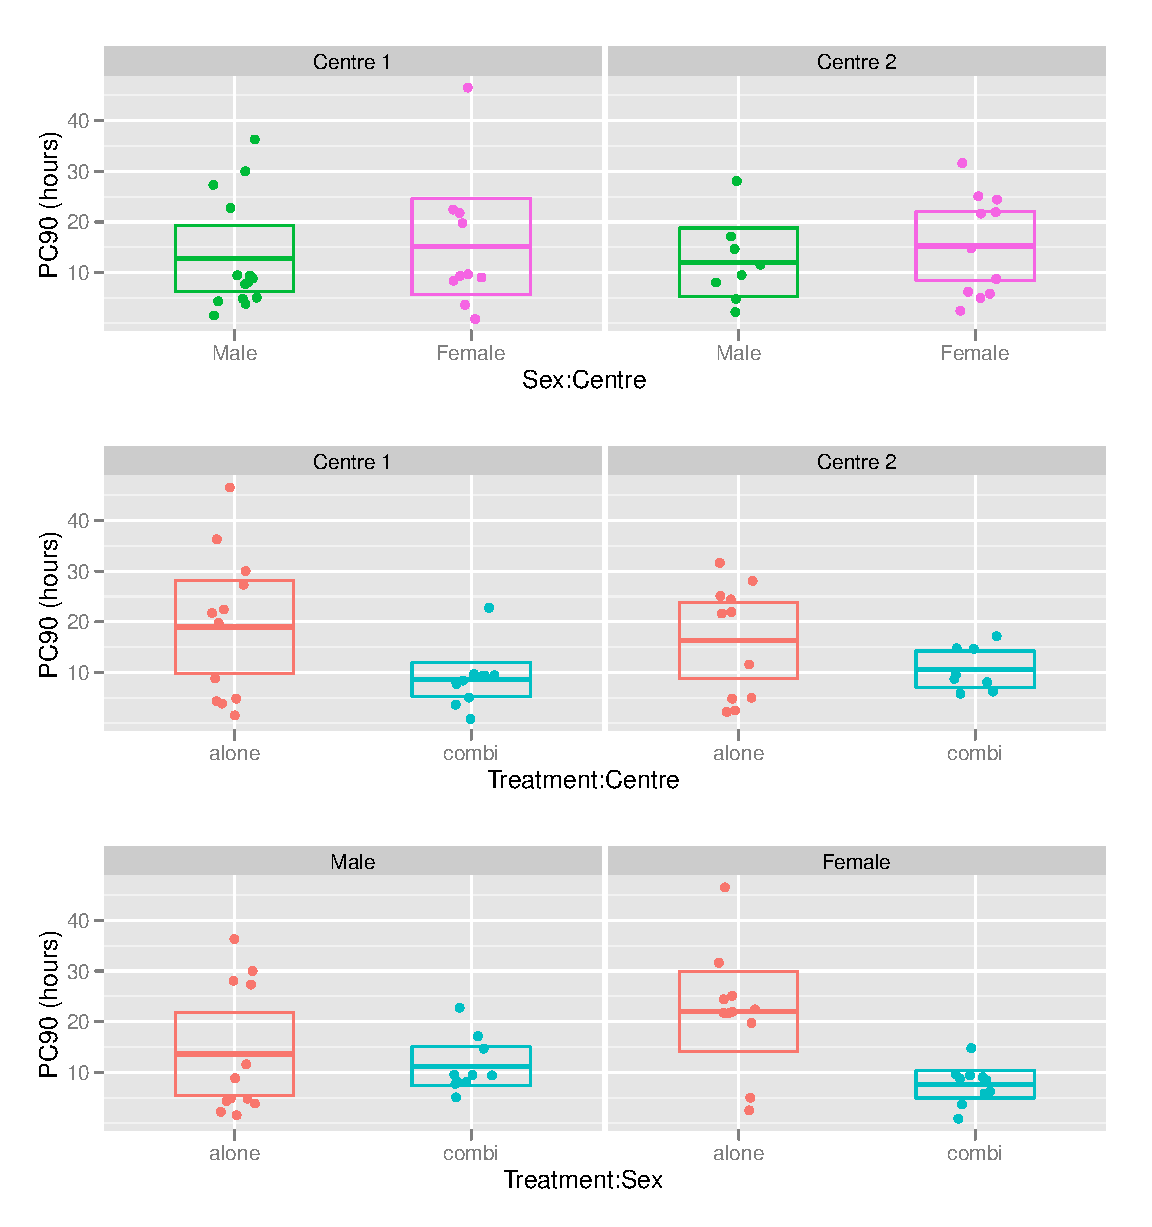
\includegraphics[width=150mm]{pc90interaction.eps} 
\caption{PC90 with 95\% confidence intervals for the means plotted by pairs of factors to look for two-way interactions}
\label{pc90interaction}
\end{figure}
It can be seen that there doesn't seem to be any interaction between sex and centre or treatment and centre i.e. the left and right panels of the top two plots look essentially the same. However, it appears that the combined treatment only decreases the mean clearance time for female subjects.
\clearpage
\section{ANOVA modelling by experimental factors}
3-way ANOVA with all interactions was performed on the PC90 data in Table \ref{derivedPC90}. The fitted model is
\begin{eqnarray}
&\mathrm{PC}90_{ijkl}=\mu+C_i+S_j+T_k+(CS)_{ij}+(CT)_{ik}+(ST)_{jk}+(CST)_{ijk}+\epsilon_{ijkl}&\nonumber\\
&\epsilon_{ijkl}\sim N(0,\sigma^2)&\label{full}
\end{eqnarray}
where PC$90_{ijkl}$ is the clearance time for subject $l$ in centre $i$, of sex $j$ on treatment $k$; $C_i$ is the effect of the centre, $S_j$ the effect of the sex; $T_k$ the treatment effect; $(CS)_{ij}$ the interaction effect of centre and sex and so on ($i,j,k=1,2$). Using a corner-point constraint, $\mu$ corresponds to the expected PC90 for a centre 1, male on the single-drug treatment, with all other terms in the model representing the difference from this mean.

The standardized residuals ($e/\hat{\sigma}$) obtained from fitting model \ref{full} are plotted in Figure \ref{aovloglinres}.
\begin{figure}[ht]
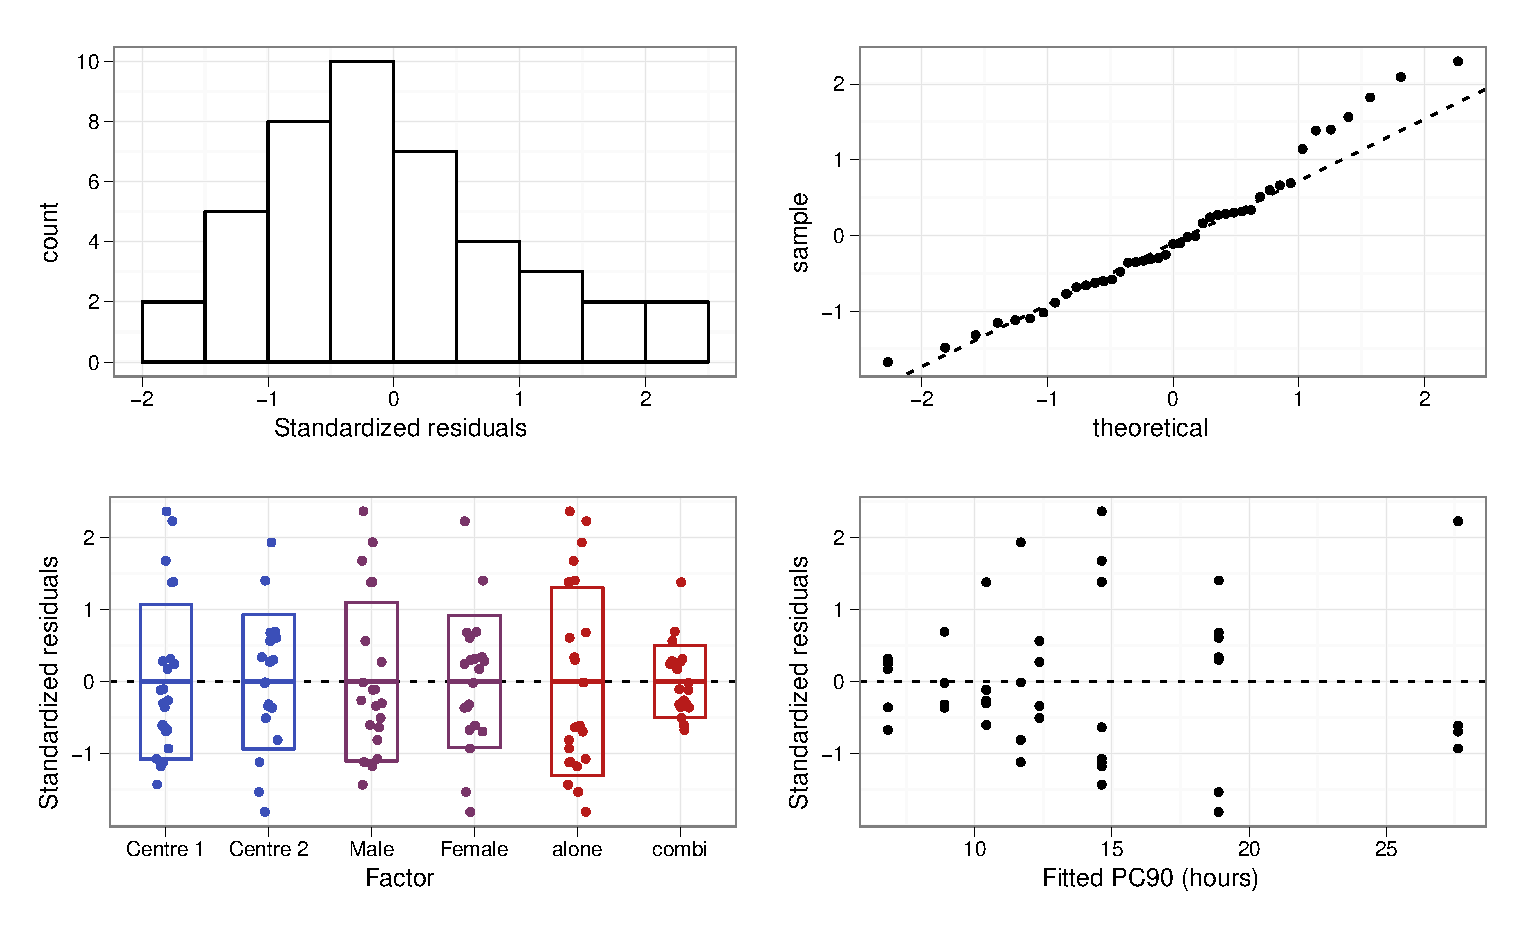
\includegraphics[width=150mm]{aovloglinres.eps} 
\caption{Residuals for 3-way ANOVA model for PC90 with all interactions}
\label{aovloglinres}
\end{figure}

It can be seen that the residuals are approximately normally distributed, but perhaps slightly right skewed. In the plot of the residuals by experimental factor (bottom-left) the standard deviation of the residuals is shown as the upper and lower edges of the rectangles. The standard deviation of standardized residuals should be approximately 1 and independent of factor. We can see that this is so for centre and sex, but there is heteroscedasticity between treatments with the residuals for the single-drug treatment showing a larger variance than for the combined-drug treatment.
%($P<0.05$ under a Breusch-Pagan test for heteroscedasticity \cite{breusch} as implemented by the \texttt{bptest} \emph{R} function \cite{lmtest}).
We can also see that the variance of the residuals increases with fitted PC90 value (bottom-right).

\subsection{Dealing with heteroscedasticity}
Least squares estimators are still unbiased under heteroscedasticity, but standard errors can be underestimated leading to incorrect inference \cite{long}. Two ways we can adapt our modelling to deal with heteroscedasticity are to transform the dependent variable and to use weighted least-squares fitting.

\subsubsection*{Transforming the dependent variable}
If we apply a square-root transformation to PC90 we obtain the residuals for the ANOVA model shown in Figure \ref{aovsqrtres}.
\begin{figure}[h]
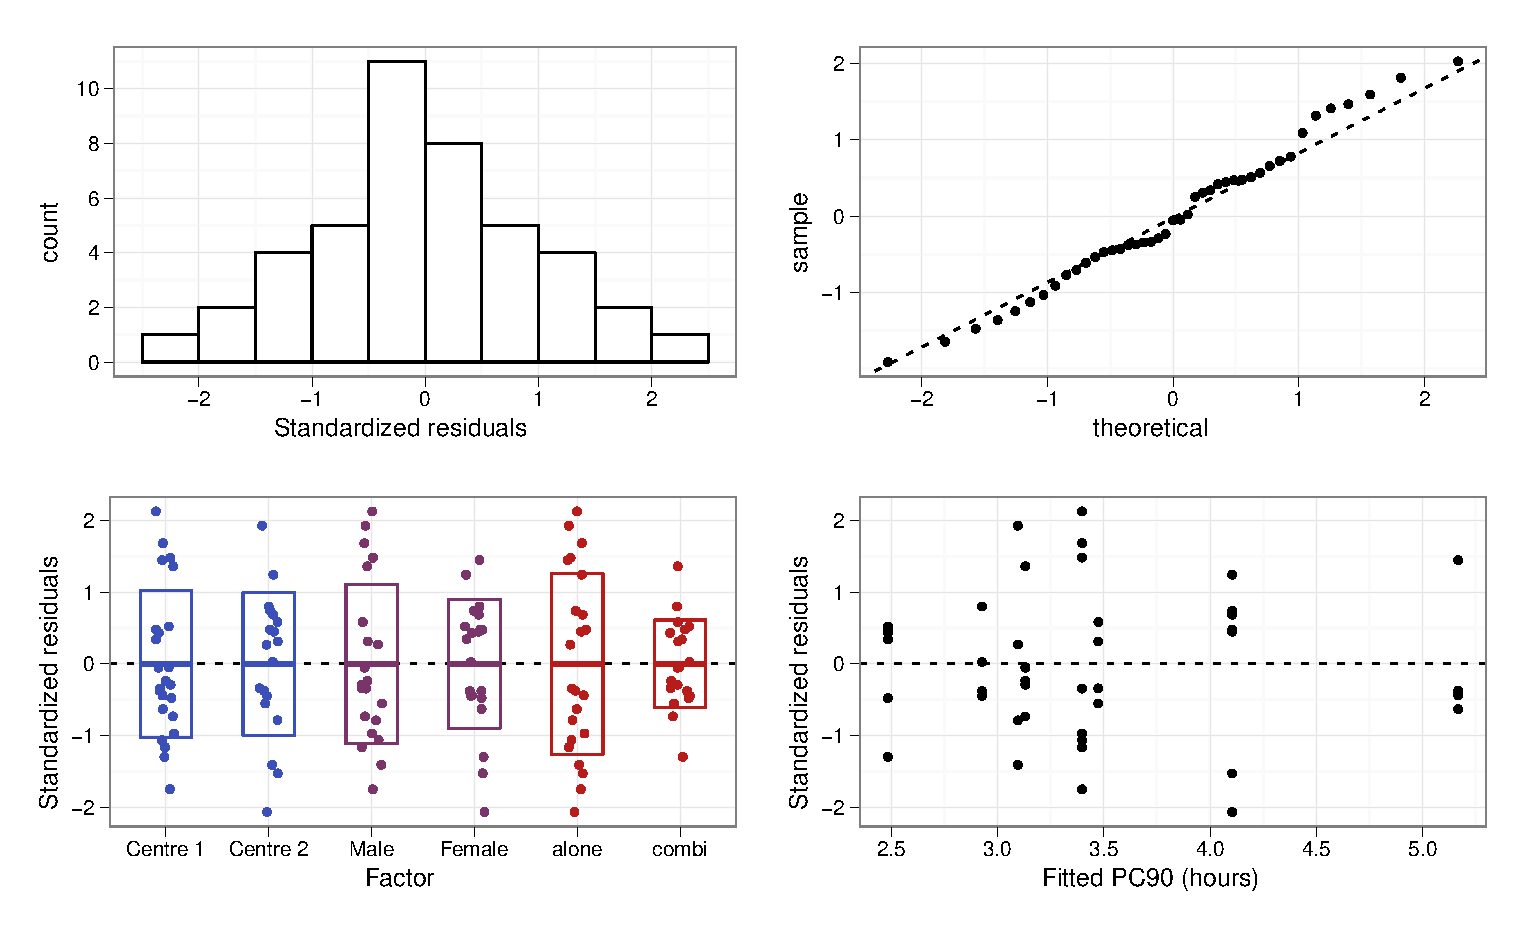
\includegraphics[width=150mm]{aovsqrtres.eps} 
\caption{Residuals after applying a square-root transformation to the dependent variable}
\label{aovsqrtres}
\end{figure}
It can be seen that this transformation reduces the correlation of the variance of the residuals with fitted PC90. Other transformations, such as logarithmic or square, did not prove as suitable as a square-root transformation. The Box-Cox method, whereby the transformation giving the highest likelihood is found, suggests transforming the dependent variable by raising it to the power 0.3 is optimal. This did not appear to give a noticeable improvement over the square-root transformation (power 0.5) in residual plots however.

It can be seen that, even after our square-root transformation, the residuals for subjects on the combined treatment have a smaller variance than for those on the single treatment. Bartlett's test for equality of variances \cite{montgomery} between the 8 ($2^{3}$) centre-sex-treatment groups gives evidence to reject the hypothesis that the variance is equal in all groups ($P<0.05$).  One common method of dealing with heteroscedastic residuals between groups is to use weighted least-squares.

\subsubsection*{Weighted least-squares}
In this case, to remedy the heteroscedasticity between treatment groups, we weight the fitting by the variance within treatment groups such that error term in model \ref{full} becomes 
\begin{equation}
\epsilon_{ijkl}\sim N(0,\sigma^2\sigma_{k}^{2})\label{wls}
\end{equation}
where $\sigma_{k=1}^{2}$ is the variance of subjects on the single treatment, $\sigma_{k=2}^{2}$ is the variance of subjects on the combined treatment and we estimate $\sigma^{2}$. This model is fitted by minimizing
\begin{equation*}
S=\sum_{ijkl} w_{k}(\mathrm{PC}90_{ijkl} - \widehat{\mathrm{PC}90_{ijk}})^{2}
\end{equation*}
where the weights $w_{k}=\sigma_{k}^{-2}$. The residuals from fitting this function using the \texttt{weights} parameter of the \emph{R} linear least-squares \texttt{lm} function are shown in Figure \ref{aovresw}.
\begin{figure}[p]
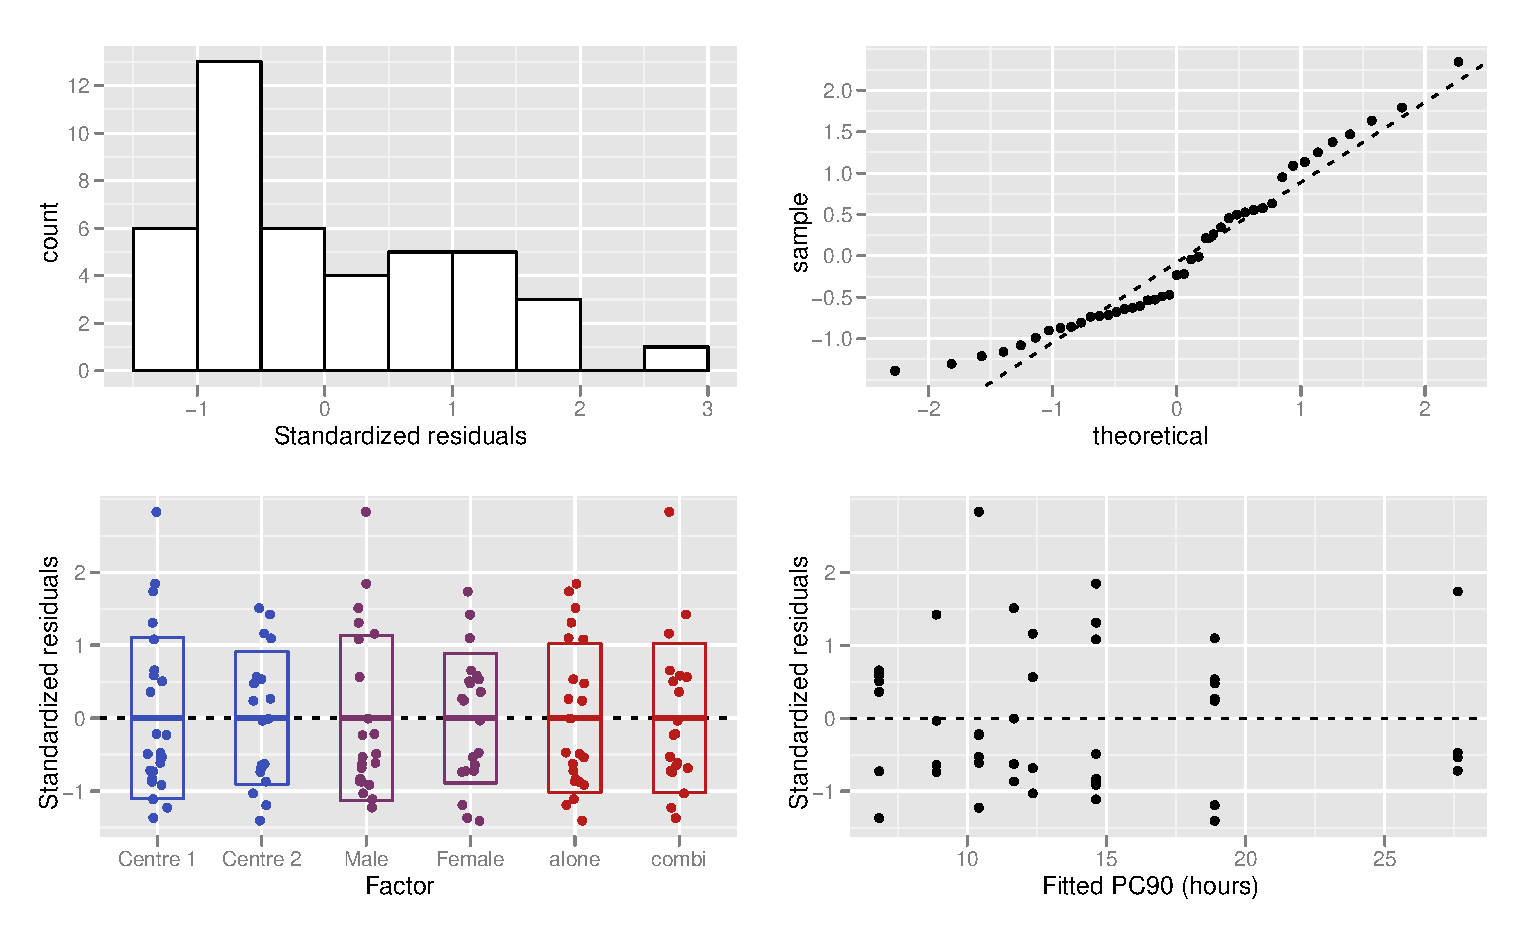
\includegraphics[width=150mm]{aovresw.eps} 
\caption{Residuals after applying weighted least squares}
\label{aovresw}
\end{figure}
The residuals now have approximately equal variance with respect to factor and fitted PC90, but they appear to be right-skewed.

If we apply the square-root transformation followed by the treatment-variance weighted least-squares fit we obtain the residuals shown in Figure \ref{aovsqrtresw}.
\begin{figure}[p]
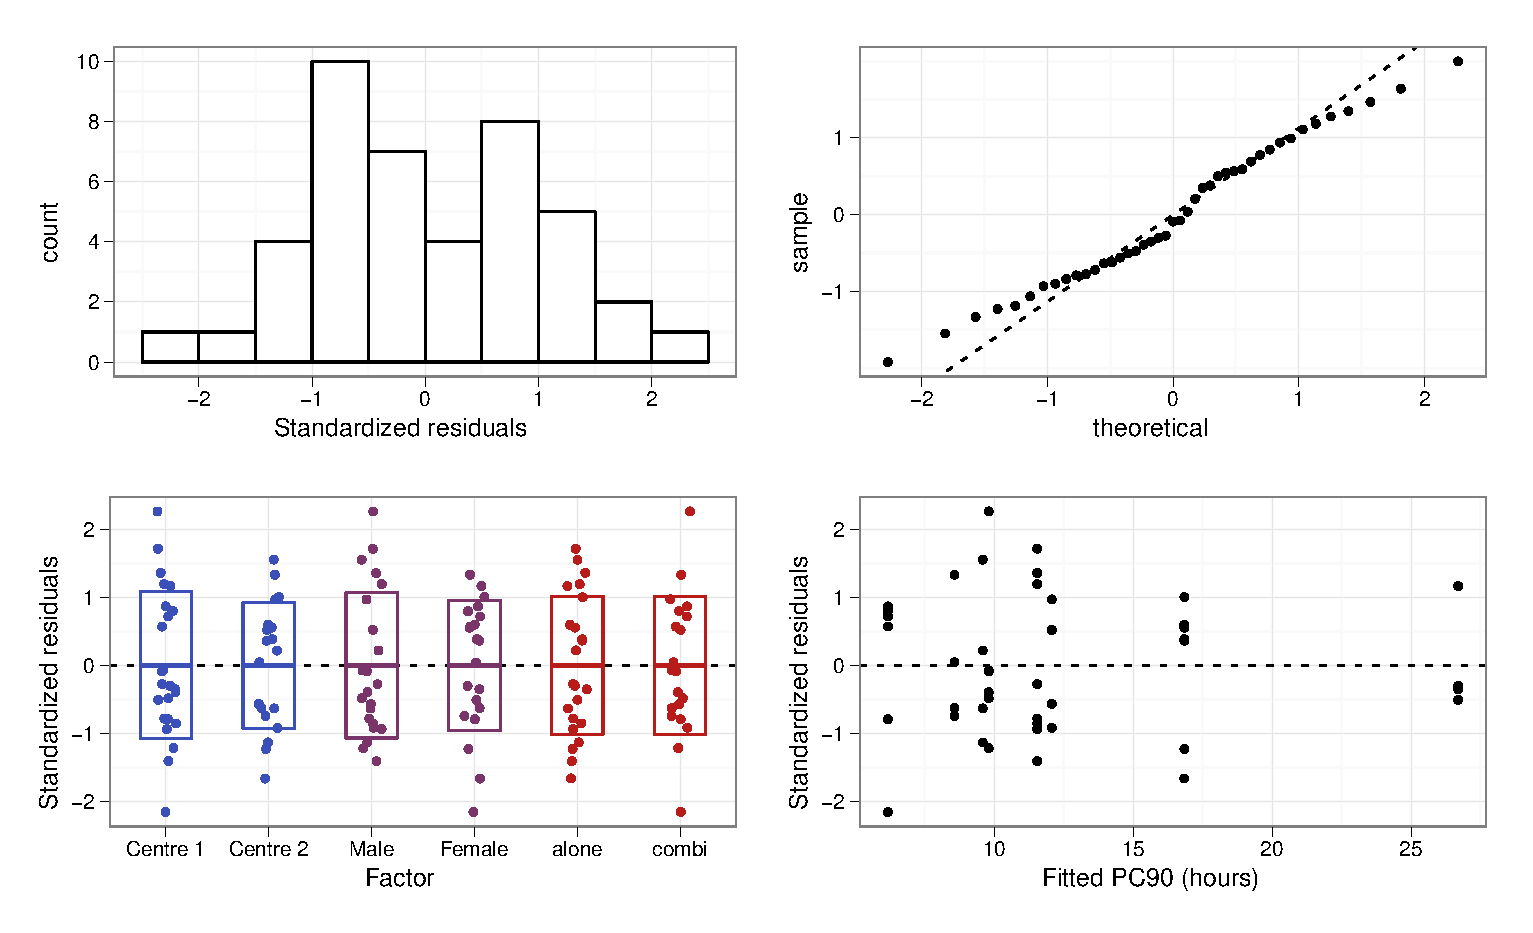
\includegraphics[width=150mm]{aovsqrtresw.eps} 
\caption{Residuals after applying square-root transformation and weighted least squares}
\label{aovsqrtresw}
\end{figure}
This seems to give a more symmetric distribution of residuals but is perhaps a bit light-tailed.
Despite this, none of the distributions of residuals show evidence of significant departures from normality by a Shapiro-Wilk test and there also now seems to be no significant difference in the variance of the residuals between experimental groups.

\subsection{Model selection}
Now that we seem to have a transformation such that the assumptions of our model are met we can start to look at hypothesis tests on the experimental factors. Table \ref{aovwt} shows the results of the ANOVA analysis for model \ref{full} using  weighted least-squares. Table \ref{aovsqrtwt} shows the results for the model using a square root transformation and weighted least-squares.
\begin{table}[h]
\centering
\caption{ANOVA table for full model fitted by weighted least-squares}\label{aovwt}
\begin{tabular}{l|rrrrrl}
Source&Sum Sq.&df&Mean Sq.&$F$&P($>F$)\\
\hline
$Centre$     &                0.631  &1& 0.631 & 0.654 &0.424&\\
$Sex$        &              0.972  &1& 0.972 & 1.01 &0.322\\
$Treatment$  &            7.85  &1& 7.85  &8.14 &0.007 &**\\
$Centre\times Sex$ &             0.001 &1&  0.001 & 0.001 &0.975&\\
$Centre\times Treatment$ &        0.511  &1& 0.511 & 0.530 &0.472&\\
$Sex\times Treatment$     &     5.21  &1& 5.21 & 5.40 &0.026 &* \\
$Centre\times Sex\times Treatment$ &   0.239 &1&  0.239 & 0.247& 0.622&\\
$Residuals$      &    33.76 &35&  0.965  &&&\\
\hline
Total&49.17&42&&&
\end{tabular}\\
\hspace{20em}*$<0.05$\quad**$<0.01$
\end{table}
\begin{table}[h]
\centering
\caption{ANOVA table for full model with square-root transformation fitted by weighted least-squares}\label{aovsqrtwt}
\begin{tabular}{l|rrrrrl}                   
Source&Sum Sq.&df&Mean Sq.&$F$&P($>F$)\\
\hline
$Centre$     &                0.834 &1&  0.834 & 0.882 & 0.354 &\\    
$Sex$        &               0.630 &1&  0.630 & 0.666 & 0.420 &\\  
$Treatment$  &            4.89 &1&  4.89 &  5.17 & 0.029& *\\
$Centre\times Sex$ &             0.003 &1& 0.003 & 0.003 & 0.956&\\
$Centre\times Treatment$ &        0.523 &1&  0.523 & 0.553 & 0.462&\\
$Sex\times Treatment$     &     5.94 &1& 5.94 & 6.28 & 0.017& *\\
$Centre\times Sex\times Treatment$ &   0.271 &1&  0.271 & 0.287 & 0.596&\\
$Residuals$      &    33.118 &35&  0.946 &&&\\
\hline
Total&46.21&42&&&
\end{tabular}\\
\hspace{20em}*$<0.05$
\end{table}

It can be seen that there is no evidence to reject the hypothesis that the centre has negligible effect on the clearance time. 
%\subsubsection*{Non-parametric check on $p$-values}
%We checked that our residuals were approximately normally distributed and homoscedastic and so our hypothesis tests and standard errors, based on these assumptions, should be accurate. However, we can perform an additional non-parametric validation by resampling methods.

%If we randomize the clearance times among the 43 patients and then refit our model and calculate the $F$ statistic for each randomization we can construct the empirical distribution of the statistic and obtain $p$-values from this. This was done using 10,000 samples and the results are shown in Table \ref{aovresamp}, where the $p$-value from the F distribution ($P_{F}$), the empirical distribution obtained by randomising ($P_{rand}$) and the empirical bootstrap distribution ($P_{boot}$), whereby instead of randomising the 43 values, we resample with replacement.
%\begin{table}[h]
%\centering
%\caption{Comparison of parametric $p$-values and $p$-values from resampling}\label{aovresamp}
%\begin{tabular}{l|rrrr|rrrrl}
%&\multicolumn{4}{c}{Weighted LSQ}&\multicolumn{4}{c}{Sqrt weighted LSQ}&\\                   
%Source&$F$&$P_{F}$&$P_{rand}$&$P_{boot}$&$F$&$P_{F}$&$P_{rand}$&$P_{boot}$&\\
%\hline
%$Centre$     						& 0.654 & 0.424 & 0.536 & 0.547     	& 0.882 & 0.354 & 0.434 & 0.437 &\\    
%$Sex$        						& 1.01   & 0.322 & 0.440 & 0.446     	& 0.666 & 0.420 & 0.498 & 0.500 &\\  
%$Treatment$ 						& 8.14   & 0.007 & 0.001 & 0.002     	& 5.17   & 0.029 & 0.012 & 0.012 &*\\
%$Centre\times Sex$ 					& 0.001 & 0.975 & 0.982 & 0.981     	& 0.003 & 0.956 & 0.962& 0.964 &\\
%$Centre\times Treatment$			& 0.530 & 0.472 & 0.322 & 0.328	& 0.553 & 0.462 & 0.381& 0.375 &\\
%$Sex\times Treatment$     			& 5.40   & 0.026 & 0.003 & 0.003	& 6.28   & 0.017 & 0.005& 0.005 &*\\
%$Centre\times Sex\times Treatment$	& 0.247 & 0.622 & 0.482 & 0.491	& 0.287 & 0.596 & 0.507& 0.516 &\\
%\hline
%\end{tabular}
%\end{table}

%It can be seen that the $p$-values obtained by the parametric and non-parametric methods are in general agreement, although the F test seems more conservative than the non-parametric tests. In all 3 cases it can be seen that there is no evidence to reject the hypothesis that the effect of the centre is negligible.

\subsubsection*{Fitting a reduced model}
As the effect of centre is negligible we refit the data with the reduced model
\begin{equation}
\sqrt{\mathrm{PC}90_{jkl}}=\mu+S_j+T_k+(ST)_{jk}+\epsilon_{jkl}\quad\quad\epsilon_{jkl}\sim N(0,\sigma^{2}\sigma_{k}^2)\label{reduced}
\end{equation}
using weighted least-squares. The residuals for this fit are shown in Figure \ref{aov2rwt}.
\begin{figure}[ht]
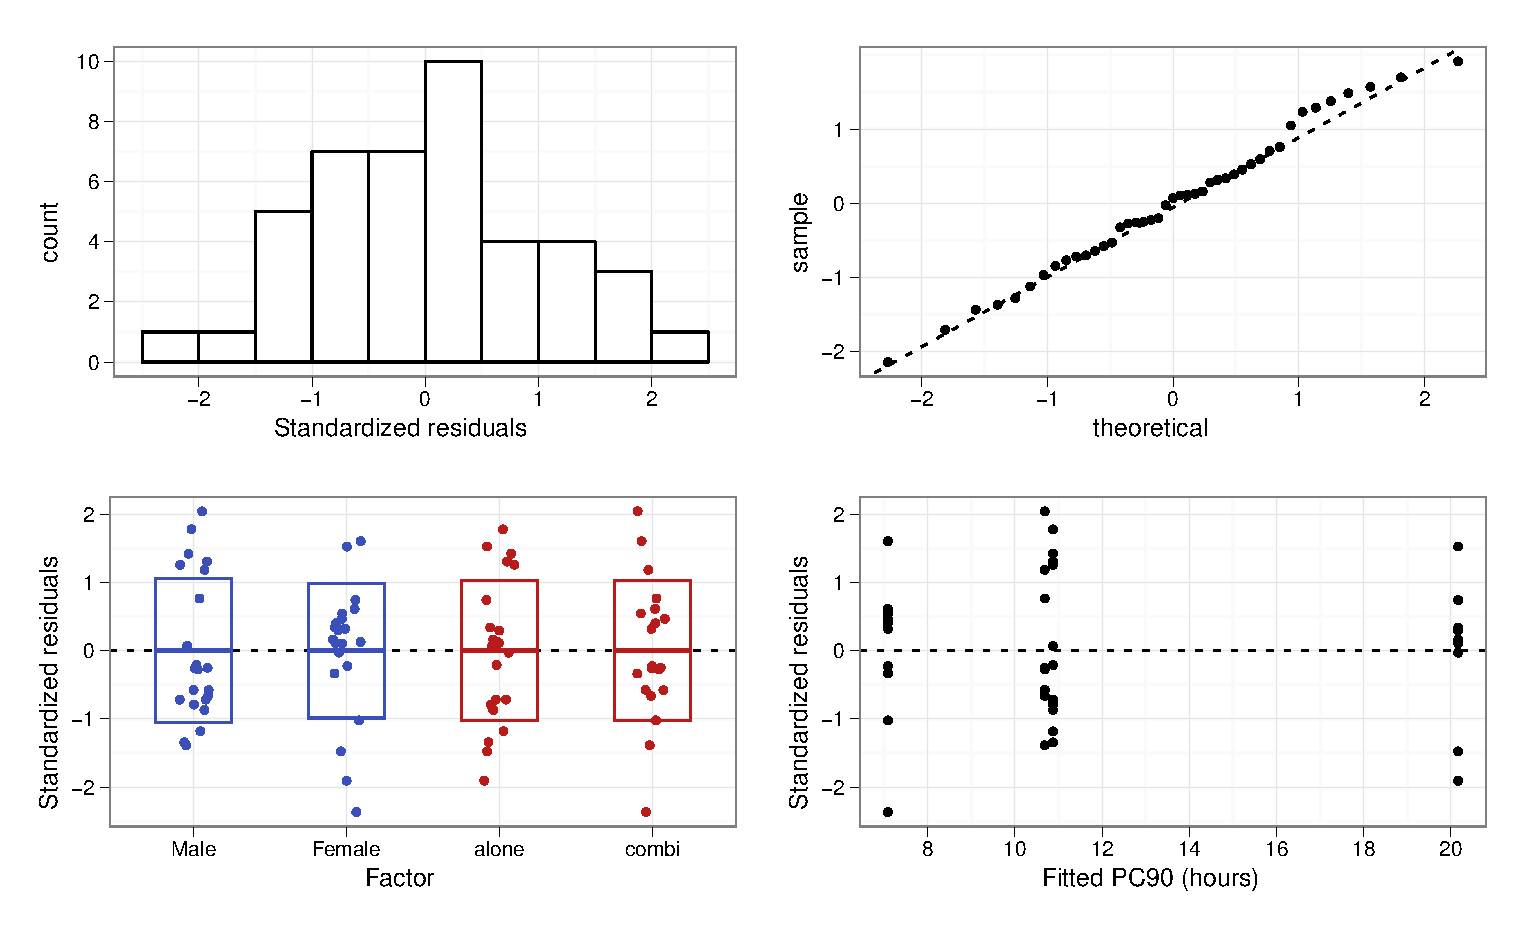
\includegraphics[width=150mm]{aov2rwt.eps} 
\caption{Residuals for the reduced model}
\label{aov2rwt}
\end{figure}

It can be seen that they are approximately normal and homoscedastic. The ANOVA table for this model is shown in Table \ref{aovreduced}, where the results are essentially the same as for the full model with some variation in the sex and treatment sums of squares due to the design matrix not being orthogonal.
%Sex            1  0.538   0.538  0.5939 0.44555  
%Treatment      1  5.152   5.152  5.6831 0.02209 *
%Sex:Treatment  1  5.166   5.166  5.6994 0.02191 *
%Residuals     39 35.353   0.906  
\begin{table}[h]
\centering
\caption{ANOVA table for the reduced model}\label{aovreduced}
\begin{tabular}{l|rrrrrl}
Source&Sum Sq.&df&Mean Sq.&$F$&P($>F$)\\
\hline
$Sex$				& 0.538 & 1 & 0.538 & 0.594 & 0.446 & \\
$Treatment$			& 5.15   & 1 & 5.15   & 5.68   & 0.022 & *\\
$Sex\times Treatment$	& 5.17   & 1 & 5.17   & 5.70   & 0.022 & *\\
$Residuals$			& 35.35 & 39 & 0.906 &&&\\
\hline
Total&46.21&42&&&
\end{tabular}\\
\hspace{20em}*$<0.05$
\end{table}

The fitted coefficients for the reduced model are shown in Table \ref{coefreduced}.
%                         Estimate Std. Error t value Pr(>|t|)    
%(Intercept)               3.29767    0.46257   7.129 1.43e-08 ***
%SexFemale                 1.19286    0.66887   1.783   0.0823 .  
%Treatmentcombi           -0.02899    0.52369  -0.055   0.9561    
%SexFemale:Treatmentcombi -1.79917    0.75363  -2.387   0.0219 *  
\begin{table}[h]
\centering
\caption{Fitted coefficients for the reduced model}\label{coefreduced}
\begin{tabular}{l|rrrc}
Factor levels&Coefficient&S.E.&$t$&P($>|t|$)\\
\hline
Male, single ($\mu$)			& 3.30 & 0.46 & 7.13 &  $1.4\times 10^{-8}$ \\
$\Delta$Female, single		& 1.19 & 0.67 & 1.78 & 0.082  \\
$\Delta$Male, combined 		& -0.029 & 0.52 & -0.055 & 0.96  \\
$\Delta$Female, combined	& -1.80 & 0.75 & -2.39 & 0.022  \\
\hline
\end{tabular}\\
Residual standard error: 0.95, Adjusted $R^{2}$: 0.18
\end{table}

With the corner-point constraint used only the male, single-treatment coefficient is absolute, with the other 3 being the relative change in $\sqrt{\mathrm{PC}90}$ with change in factor level (indicated by $\Delta$). The $p$-values are perhaps a bit misleading in that the $p$-value for the mean $\mu$ corresponds to the null hypothesis $\mu=0$, with the other $p$-values corresponding to the hypotheses that the change in clearance time from the mean is 0 due to each change in factor level. Therefore, although only the female, combined treatment appears to be significantly different from the male, single treatment (-1.80), the mean difference between females on the single and combined treatments is larger i.e. $1.19-(-1.80)=2.99$. However, it is clear that there is no evidence to reject the hypothesis that the combined treatment gives the same mean clearance time as the single treatment for males.

Looking at inference for the clearance times will give a clearer picture of the relative effects of the factors.

\subsection{Inference for Clearance Times}
%\begin{itemize}
%\item The mean clearance time for male patients on the single treatment is $3.30^{2}=10.88$ hours with a 95\% confidence interval of ($2.54^{2},\ 4.05^{2})=(6.47,\ 16.41)$ hours.
%\item There is no evidence to reject the hypothesis that there is no difference between mean clearance times for male subjects on the single and combined treatments.
%\item Female subjects on the single treatment have a mean clearance time of $(3.30+1.19)^{2}=20.16$ hours with a 95\% confidence interval of (13.72, 27.85) hours.
%\item Female subjects on the combined treatment have a mean clearance time of $(3.30+1.19-0.029-1.80)^{2}=7.09$ hours with a 95\% confidence interval of (3.37, 12.16) hours.
%\end{itemize}
%$hours
%  fit lwr upr
%1  10   5  17
%2  20  12  29
%3  10   7  14
%4   7   4   9

%$minutes
%  fit lwr upr
%1  52  35  55
%2  10  21  54
%3  41  41  11
%4   5  41  59
Bearing in mind that a square-root transformation was used, we have from Table \ref{coefreduced}, the mean clearance times for each sex and treatment combination with 95\% confidence intervals shown in Table \ref{inference}.
\begin{table}[h]
\centering
\caption{Mean clearance times by sex and treatment}\label{inference}
\begin{tabular}{|l|c|c|}
\hline
&Clearance time PC90&95\% conf. int.\\
Factor levels&(hrs:mins)&(hrs:mins)\\
\hline
Male, single treatment 		& 10:52 & (5:35, 17:55) \\
Female, single treatment		& 20:10 & (12:21,  29:54) \\
Male, combined treatment	& 10:41 & (7:41, 14:11) \\
Female, combined treatment	& 7:05 & (4:41, 9:59) \\
\hline
\end{tabular}
\end{table}

It should be noted that these are confidence intervals for the estimate of the mean clearance time for the population. Prediction intervals for the expected clearance time of any one subject are considerably wider i.e. 95\% prediction intervals are: Male, single (0, 44) hours; Female, single (1, 62) hours; Male, combined (3, 24) hours; Female, combined (1, 19) hours.

The mean difference in $\sqrt{\mathrm{PC}90}$ between treatment groups, with confidence intervals and $p$-values calculated by Tukey's test for comparison of means \cite{montgomery} using the \texttt{TukeyHSD} \emph{R} function are shown below.
%                           diff   lwr   upr p adj
%Female:alone-Male:alone    1.19 -0.25  2.64  0.14
%Male:combi-Male:alone     -0.03 -1.51  1.45  1.00
%Female:combi-Male:alone   -0.64 -2.12  0.85  0.66
%Male:combi-Female:alone   -1.22 -2.73  0.29  0.15
%Female:combi-Female:alone -1.83 -3.34 -0.32  0.01
%Female:combi-Male:combi   -0.61 -2.15  0.94  0.72
\begin{table}[h]
\centering
%\caption{Difference in $\sqrt{\mathrm{PC}90}$ by Tukey's test}\label{tukey}
\begin{tabular}{l|ccrl}
&Diff.&95\% CI&$p$ adj.&\\
\hline
Male: combi - single 	& -0.03 & (-1.51, 1.45) & 1.00 &\\
Female: combi - single	& -1.83 & (-3.34,  -0.32) & 0.012 &*\\
\end{tabular}\\
*$<0.05$
\end{table}

It can be seen that there is evidence to reject the hypothesis of no difference between treatment groups for female subjects ($P<0.05$).

\newpage
Therefore, we can summarize the relative effects of the single and combined treatments:
\begin{description}
%> median(rnorm(1000000, 3.297668, 0.4625680)^2 - rnorm(1000000, 3.268677, 0.2455219)^2)
%[1] 0.1926644
%> mean(rnorm(1000000, 3.297668, 0.4625680)^2 - rnorm(1000000, 3.268677, 0.2455219)^2)
%[1] 0.34226
%> quantile(rnorm(1000000, 3.297668, 0.4625680)^2 - rnorm(1000000, 3.268677, 0.2455219)^2, probs=c(0.025,0.975))
%    2.5%    97.5% 
%-5.99823  7.56040 
\item[Male subjects] - There is no evidence of a difference in mean clearance times between the two treatments for male subjects. The mean difference in clearance times for male subjects on the combined treatment is 0.3 hours shorter (median 0.2 hours) than for those on the single treatment with a 95\% confidence interval of (-6.0, 7.6) hours shorter.
%> median(rnorm(1000000, 4.490531, 0.4831365)^2 - rnorm(1000000, 2.662371, 0.2455219)^2)
%[1] 13.03766
%> mean(rnorm(1000000, 4.490531, 0.4831365)^2 - rnorm(1000000, 2.662371, 0.2455219)^2)
%[1] 13.25602
%> quantile(rnorm(1000000, 4.490531, 0.4831365)^2 - rnorm(1000000, 2.662371, 0.2455219)^2, probs=c(0.025,0.975))
%     2.5%     97.5% 
% 4.960203 22.749181
\item[Female subjects] - The mean difference in clearance times for female subjects on the combined treatment is 13.2 hours shorter (median 13.0 hours) than for those on the single treatment with a 95\% confidence interval of (5.0, 22.7) hours shorter.
\end{description}

The confidence intervals for the difference between groups in hours (i.e. the original scale before the square-root transformation used for the regression) are obtained by sampling 10,000 values from each of $[N(m_{a},s_{a}^{2})]^{2}$ and $[N(m_{b},s_{b}^{2})]^{2}$, where $a$ and $b$ specify the groups and $m$ and $s$ are the estimated mean and standard error of $\sqrt{\mathrm{PC}90}$ in the groups. The percentiles of the distribution of the differences between these two samples are then taken. The median is given as the distribution will be right-skew when transformed back to hours, although not by much; we see above that medians and means are fairly close.

\subsection{Comparison with other PC90 estimation methods}
The graphical investigation and model fitting procedure was repeated with the PC90 estimates obtained using the cubic polynomial and logistic regression techniques. The same overall trend and patterns of residuals were observed, leading to selection of the same optimal model (Equation \ref{reduced} on page \pageref{reduced}). The fitted coefficients are compared in Table \ref{compmeth}. 
\begin{table}[h]
\centering
\caption{Comparison of fitted models by 2 PC90 estimation methods}\label{compmeth}
\begin{tabular}{l|rr|rr|rr}
&\multicolumn{2}{c|}{log-linear}&\multicolumn{2}{c|}{cubic}&\multicolumn{2}{c}{logistic}\\
Factor levels&Coefficient&S.E.&Coefficient&S.E.&Coefficient&S.E.\\
\hline
Male, single ($\mu$)			& 3.30 & 0.46 & 3.43 &  0.49 & 4.06 & 0.52\\
$\Delta$Female, single		& 1.19 & 0.67 & 1.02 & 0.70  & 0.49 & 0.81\\
$\Delta$Male, combined		& -0.029 & 0.52 & -0.077 & 0.55 & -0.64 & 0.57\\
$\Delta$Female, combined	& -1.80 & 0.75 & -1.68 & 0.79  & -1.11 & 0.88\\
\hline
\end{tabular}
\end{table}

It can be seen that there is good agreement between the models fitted to the clearance times estimated by the log-linear and cubic methods. The estimated mean clearance times are compared in Table \ref{compinf}. Generally the same conclusions can be drawn regarding treatment effectiveness for the three methods, with the exception of male, single subjects with the logistic method. Remember that the logistic data has 8 subjects missing, all from the single treatment group, which most likely explains this discrepancy.
\begin{table}[h]
\centering
\caption{Mean clearance times by sex and treatment (hrs:mins)}\label{compinf}
\begin{tabular}{|l|cc|cc|cc|}
\hline
&\multicolumn{2}{c|}{log-linear}&\multicolumn{2}{c|}{cubic}&\multicolumn{2}{c|}{logistic}\\
Level		&Mean&95\% CI&Mean&95\% CI&Mean&95\% CI\\
\hline
M, single 		& 10:52 & (5:35, 17:55) &11:47& (6:00, 19:30) & 16:28 &(9:03, 26:05)\\
F, single		& 20:10 & (12:21,  29:54) &19:52&(11:46, 30:04) & 20:41&(10:38, 34:02)\\
M, combi	 	& 10:41 & (7:41, 14:11) &11:16&(8:02, 15:02) & 11:41 &(8:37, 15:13)\\
F, combi	 	& 7:05 & (4:41, 9:59) &7:16&(4:44, 10:21) & 7:49 & (5:21, 10:46)\\
\hline
\end{tabular}
\end{table}

\section{Dependence of clearance time on pre-dose parasite count}
\subsubsection*{Pre-dose count}\label{sec:predoseancova}
We might expect that subjects with a higher pre-dose parasite count would have a longer clearance time. To investigate this, the PC90 clearance time is plotted against pre-dose parasite count in Figure \ref{predose-ancova}. There is no obvious trend in clearance time with pre-dose parasite, nor when the data is split by centre, sex and treatment. Statistical tests such as Spearman's rho and ANCOVA (adding pre-dose count as a covariate to the ANOVA model) do not give any evidence of correlation of clearance time with pre-dose parasite count.
\begin{figure}[p]
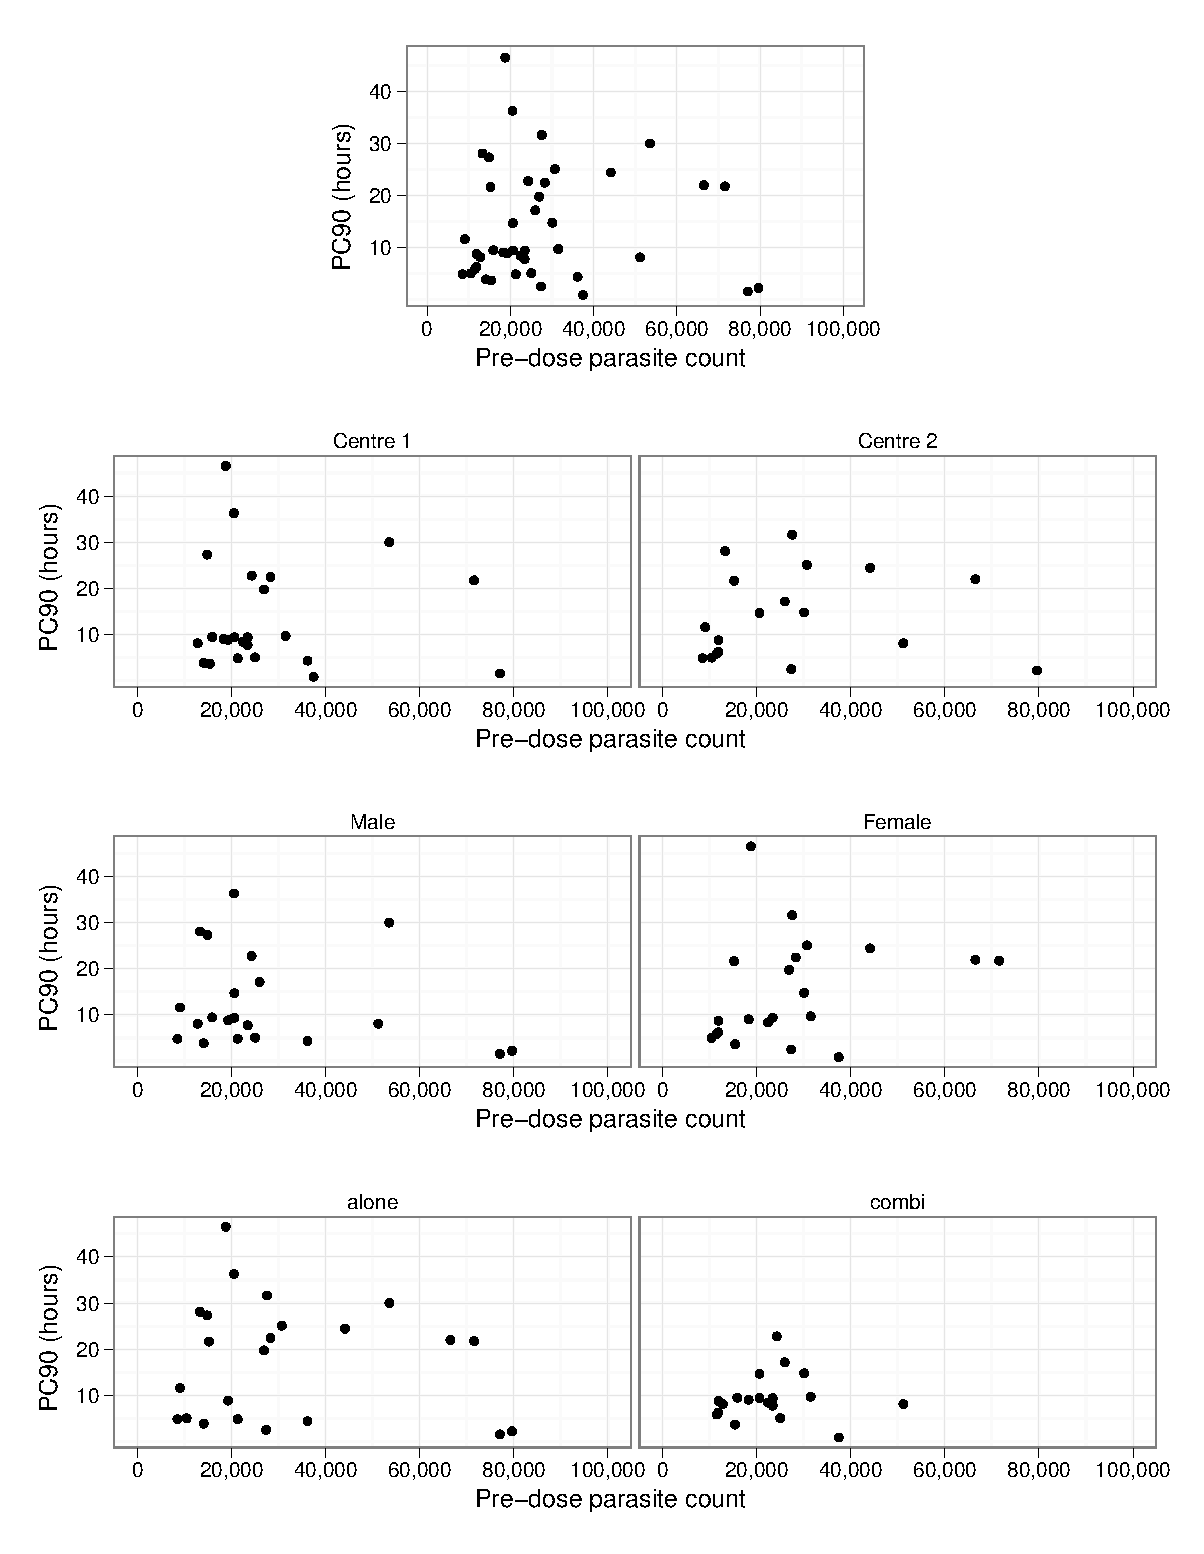
\includegraphics[width=150mm]{predose-ancova.eps} 
\caption{Dependence of clearance time on pre-dose parasite count}
\label{predose-ancova}
\end{figure}

%The fitted ANCOVA model is a modification of the reduced ANOVA model \ref{reduced} on page \pageref{reduced} adding the pre-dose parasite count as a covariate with all interactions with sex and treatment. This ANCOVA model is compared to the ANOVA model in Figure \ref{compancova}. It can be seen that the ANCOVA model isn't a significant improvement.

\subsubsection*{Time of pre-dose count}\label{sec:pretimeancova}
The clearance time is plotted against the time before first dose at which the pre-dose count was recorded in Figure \ref{pretime-ancova}. Although it looks like there is some positive correlation between the time of pre-dose recording and clearance times, statistical tests reveal no evidence to reject the hypothesis that the effect of pre-dose recording time is negligible. It could be that we do not have enough power with this sample to detect an effect if there is one. 
\begin{figure}[p]
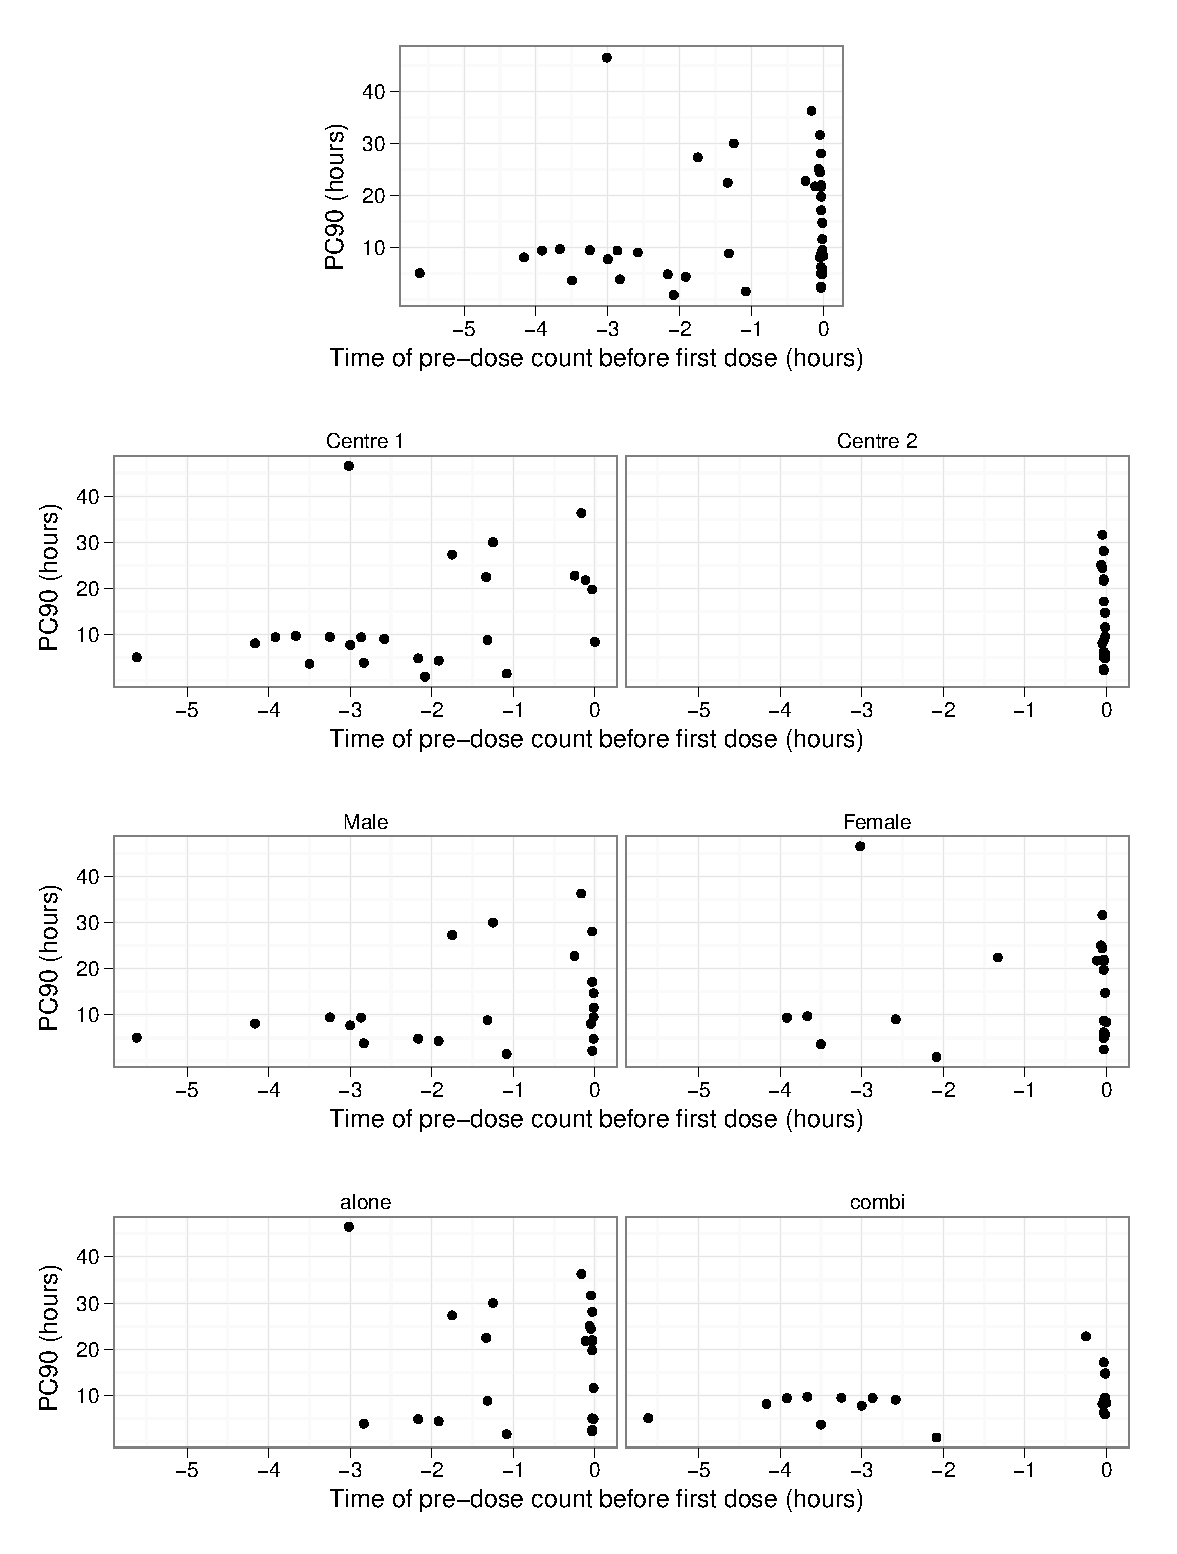
\includegraphics[width=150mm]{pretime-ancova.eps} 
\caption{Dependence of clearance time on the time before first dose that the pre-dose parasite count was recorded}
\label{pretime-ancova}
\end{figure}

%The ANCOVA model with time of pre-dose count as a covariate is compared to the ANOVA model in Figure \ref{compancova2}.
%It looks like there is a significant interaction with time of pre-dose count for female subjects, but this is mainly attributed to a single high-leverage datum and the coefficient in the ANCOVA model isn't highly significant ($p$=0.077). It could be that we simply don't have high enough power in this experiment to detect this interaction.

%\begin{figure}[p]
%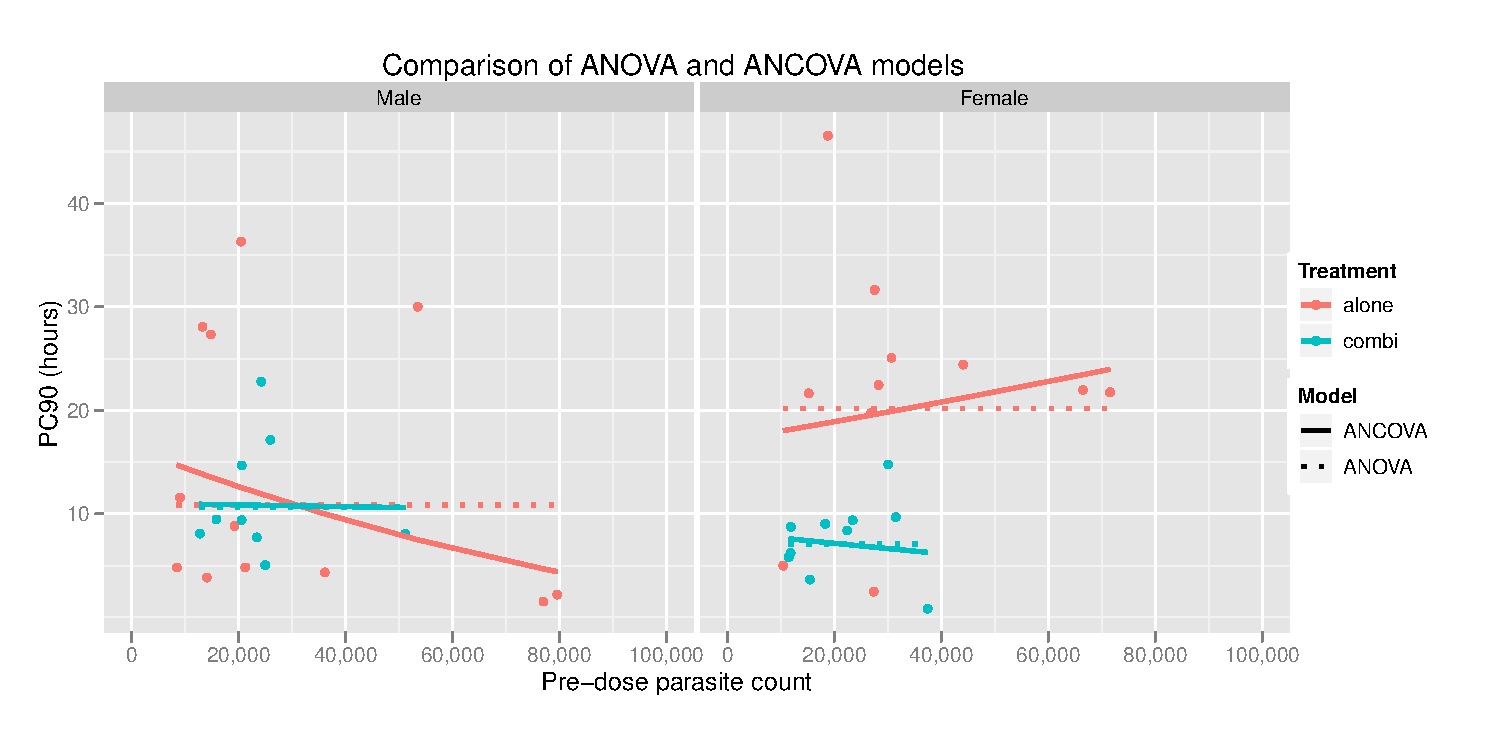
\includegraphics[width=150mm]{compancova.eps} 
%\caption{Comparison of ANOVA and ANCOVA models}
%\label{compancova}
%\end{figure}
%\begin{figure}[p]
%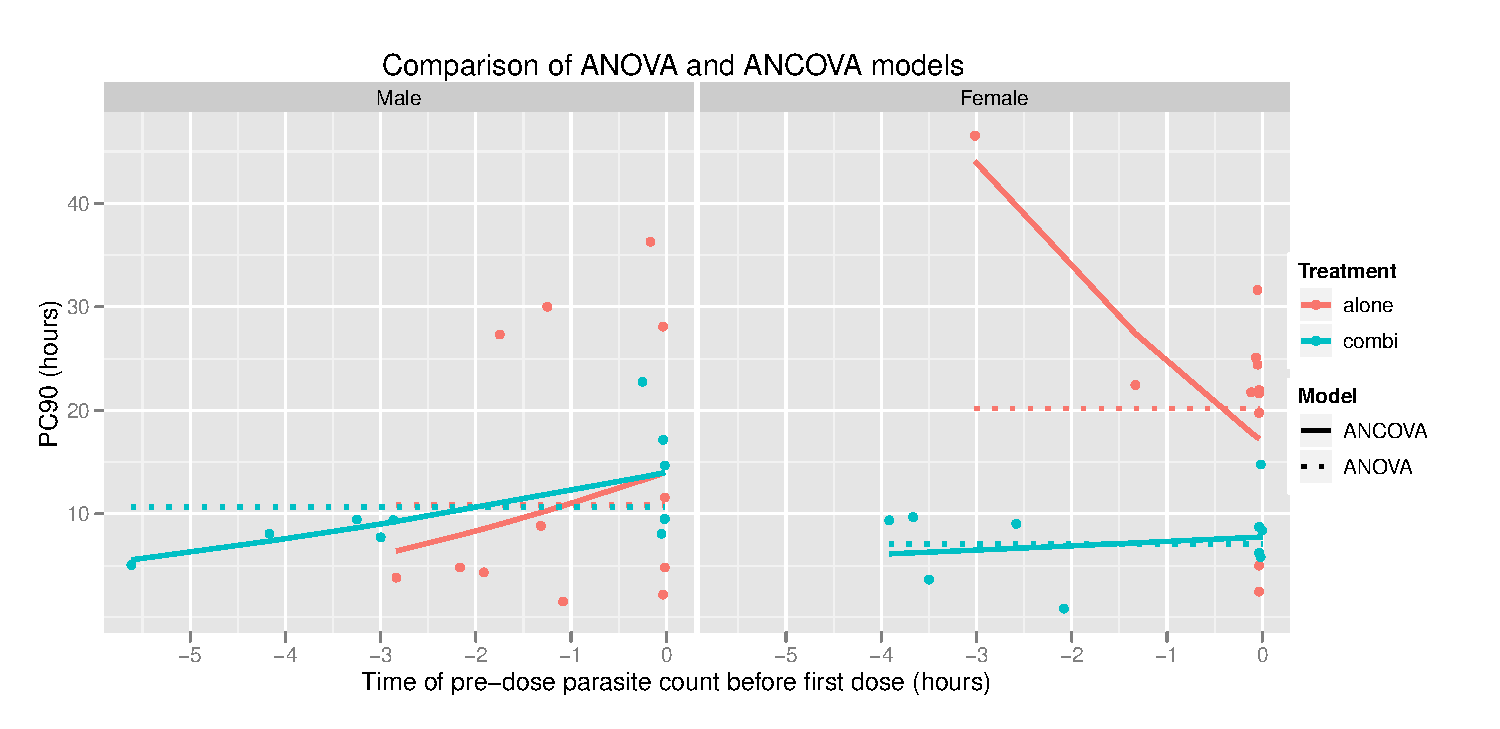
\includegraphics[width=150mm]{compancova2.eps} 
%\caption{Comparison of ANOVA and ANCOVA models}
%\label{compancova2}
%\end{figure}
\clearpage
\section{Non-parametric methods}
As an additional verification of the analysis so far based on parametric methods, we can compare the results with analysis of clearance times using non-parametric, distribution-free methods.

\subsection{Non-parametric statistics}
\subsubsection*{ANOVA using ranks}
One non-parametric alternative to two-way ANOVA is to calculate the $F$ statistics using the ranks of the data instead of the actual values of the dependent variable \cite{conover}. The results of ANOVA using ranks are shown in Table \ref{aovranks} with the $p$-values from the parametric analysis (Table \ref{aovreduced} on page \pageref{aovreduced}) shown for comparison.
%> summary(PC90.loglinr.rank.aov)
%              Df Sum Sq Mean Sq F value  Pr(>F)  
%Sex            1   78.3    78.3  0.5562 0.46025  
%Treatment      1  390.6   390.6  2.7758 0.10371  
%Sex:Treatment  1  664.9   664.9  4.7247 0.03587 *
%Residuals     39 5488.2   140.7    
\begin{table}[h]
\centering
\caption{ANOVA using ranks}\label{aovranks}
\begin{tabular}{l|rrrrrl|rl}
Source&Sum Sq.&df&Mean Sq.&$F$&P($>F$)&&P$^{\dag}$($>F$)\\
\hline
$Sex$				& 78.3 & 1 & 78.3 & 0.556 &  0.460 && 0.446& \\
$Treatment$			& 390.6   & 1 & 390.6   & 2.78 & 0.104&  & 0.022&* \\
$Sex\times Treatment$	& 664.9   & 1 & 664.9   & 4.72 & 0.036&*   & 0.022&* \\
$Residuals$			& 5488.2 & 39 & 140.7 &&&&\\
\hline
Total&6622&42&&&&
\end{tabular}\\
P$^{\dag}$: $p$-value from parametric analysis\qquad*$<0.05$
\end{table}

It can be seen that the non-parametric method shows a significant interaction effect at the 5\% level, but not for the main treatment effect unlike the parametric analysis. It could be that there is only an effect of treatment for one sex (Figure \ref{pc90interaction} on page \pageref{pc90interaction} would suggest this), although Toothaker \textit{et al.} \cite{toothaker} note that these tests should not be used to test for main effects in the presence of an interaction and vice-versa.

\subsection{Resampling methods}\label{section:resampling}
Another alternative to parametric ANOVA is to resample the data using either the permutation or bootstrap methods and thereby determine the sampling distribution of our statistics \cite{manly}. There are several different approaches for resampling ANOVA models with crossed factors, such as ours, by permutation \cite{manly, anderson}. Three of them are:
\begin{description}
\item[Unrestricted permutation of raw data] - The raw data is randomized between all groups and the $F$ statistics recalculated for each randomization. Anderson and Braak note that this is an approximate test for both main effects and interactions \cite{anderson}.
\item[Permutation of residuals] - An approximate test for an interaction effect by controlling for main effects can be performed by defining residuals
$$r_{ijk}=y_{ijk}-\bar{y}_{i..}-\bar{y}_{.j.}+\bar{y}_{...}$$
where $\bar{y}_{i..}$ is the mean response at level $i$ of the first factor, $\bar{y}_{.j.}$ the mean response at level $j$ of the second factor and $\bar{y}_{...}$ the overall mean. The $F$ statistics are then calculated from ANOVA using these residuals as the response.
\item[Restricted permutation of raw data] - To test for a main effect the response can be randomized \emph{between} levels of the main effect but \emph{within} the levels of the other factors. For example, to test for a treatment main effect with our data, we would randomize the treatment of each observation but keep the sex and centre static. Only the $F$ statistic of the main effect being randomized is relevant in the ANOVA output from this method. Anderson and Braak note that this is an exact test for main effects, but is only reasonable if there is no evidence of an interaction effect \cite{anderson}.
\end{description}
Manly finds by simulation that the $F$ statistic gives the most consistent results across all three methods, as opposed to using mean square residuals for example \cite{manly}. Anderson and Braak note that permutation of residuals is significantly more powerful that permutation of raw data when errors are highly non-normal, for example lognormal \cite{anderson}.

These 3 permutation methods were implemented in \emph{R}\footnote{The code is listed in Appendix \ref{R:resamp} on page \pageref{R:resamp}.}. The results for the full 3-way ANOVA model are shown in Table \ref{aovresamp} compared to the parametric $F$ test for the square-root transformed model fitted by weighted least-squares.
\begin{table}[h]
\centering
\caption{$p$-values for 3-way ANOVA $F$ statistic determined by resampling.\\Values not relevant to test in \small{\textit{small italics}} (see Note on page \pageref{resampnote}).}\label{aovresamp}
\begin{tabular}{l|rrrr|r}                   
Source						&P($>F_{1}$)&P($>F_{2}$)&P($>F_{3t}$)&P($>F_{3s}$)&P$^{\dag}$($>F$)\\
\hline
$Centre$     					& 0.971 & \small{\textit{0.720}} & \small{\textit{0.008}} & \small{\textit{0.173}} & 0.354 \\    
$Sex$        					& 0.370 & \small{\textit{0.912}} & \small{\textit{0.008}} & 0.364 & 0.420 \\  
$Treatment$  					& 0.009 & \small{\textit{0.962}} & 0.007 			   & \small{\textit{0.126}} & 0.029 \\
$Centre\times Sex$ 				& 0.781 & 0.780 			& \small{\textit{0.174}} & \small{\textit{0.774}} & 0.956 \\
$Centre\times Treatment$ 		& 0.361 & 0.352 			& \small{\textit{0.334}} & \small{\textit{0.113}} & 0.462 \\
$Sex\times Treatment$     		& 0.026 & 0.027 			& \small{\textit{0.027}} & \small{\textit{0.029}} & 0.017 \\
$Centre\times Sex\times Treatment$& 0.634 & 0.637 			& \small{\textit{0.629}} & \small{\textit{0.607}} & 0.596
\end{tabular}\\
$F_{1}$ - Unrestricted permutation; $F_{2}$ - Permutation of residuals; $F_{3t}$ - Permutation restricted to treatment; $F_{3s}$ - Permutation restricted to sex; P$^{\dag}$ - Parametric result\\
10,000 samples for each method
\end{table}
\begin{description}
\item[Note]\label{resampnote} --- The $p$-values not relevant to test in each row are in small italics. As discussed above, some of the resampling methods are designed for testing specific main effects and some for interactions. In a resampling method geared for testing an interaction or a specific main effect, the $p$-value returned for other main effects is not correct. Although they are incorrect (e.g. test for treatment main effect returns $P=0.008$ for centre and sex effects), they are shown to demonstrate what sort of spurious conclusions can arise if these methods are used for inappropriate tests.
\end{description}

It can be seen that the $p$-values obtained by resampling lead to the same conclusions as the parametric test. In particular that there is no evidence to reject the hypothesis that the effect of centre is negligible. Accordingly, the results for the reduced 2-way model are shown in Table \ref{aovresampr}.
\begin{table}[h]
\centering
\caption{$p$-values for 2-way ANOVA $F$ statistic determined by resampling.\\Values not relevant to test in \small{\textit{small italics}} (see Note on page \pageref{resampnote}).}\label{aovresampr}
\begin{tabular}{l|rrrr|r}                   
Source						&P($>F_{1}$)&P($>F_{2}$)&P($>F_{3t}$)&P($>F_{3s}$)&P$^{\dag}$($>F$)\\
\hline
$Sex$        					& 0.375 & \small{\textit{0.951}} & \small{\textit{0.004}} & 0.360 & 0.446 \\  
$Treatment$  					& 0.007 & \small{\textit{0.981}} & 0.007 			   & \small{\textit{0.086}} & 0.022 \\
$Sex\times Treatment$     		& 0.049 & 0.049 			& \small{\textit{0.049}} & \small{\textit{0.041}} & 0.022 \\
\end{tabular}\\
$F_{1}$ - Unrestricted permutation; $F_{2}$ - Permutation of residuals; $F_{3t}$ - Permutation restricted to treatment; $F_{3s}$ - Permutation restricted to sex; P$^{\dag}$ - Parametric result\\
10,000 samples for each method
\end{table}
It can be seen that the hypothesis tests for main effects and interactions produce the same results at the 5\% level for all the permutation techniques and the parametric model. For the permutation  methods the interaction effect is only just significant at the 5\% level. Anderson and Braak \cite{anderson} note that the parametric $F$ test is more powerful than permutation techniques when the residuals are approximately normal, as they are for our square-root transformed model fitted by weighted least-squares (Figure \ref{aov2rwt} on page \pageref{aov2rwt}).

\subsubsection*{Non-parametric confidence intervals}
Our parametric 2-way ANOVA identified that there is only a significant difference between the clearance times of the two treatments for female patients and we derived confidence intervals for the reduction in clearance time for female patients using the combined drug treatment (page \pageref{compinf}).

We can derive a non-parametric confidence interval for the improvement in clearance time for female patients using the combined treatment by resampling. If we select only female subjects and permute the clearance times between treatments then we can derive a sampling distribution of the difference between means under the null hypothesis
$$H_{0}:\mu_{s}-\mu_{c}=0$$
i.e. the mean clearance time for the single treatment $\mu_{s}$ is the same as that for the combined treatment $\mu_{c}$. To test the hypothesis that the difference between the treatments is $k$ we use the null hypothesis
$$H_{0}:\mu_{s}-\mu_{c}-k=0$$
and accordingly subtract $k$ from the clearance times for the single treatment before permuting the values. Now 95\% confidence intervals for the difference between treatments are equal to the minimum and maximum values of $k$ that are not rejected by our test at the 5\% level. Therefore, the algorithm to find the confidence interval is:
\begin{enumerate}
\item Choose a value of $k$ that we think is at the 95\% confidence limit for the difference between clearance times. Good initial choice are the limits from the parametric test.
\item Subtract $k$ from the original clearance times for the single treatment.\label{start}
\item Calculate the statistic $T_{obs}=\mu_{s}-\mu_{c}$.\label{fstat}
\item Permute the clearance times between treatments $N-1$ times and at each permutation calculate $T^{*}_{i}=\mu_{s}^{*}-\mu_{c}^{*}$.
\item Calculate the $p$-value of our $T_{obs}$ statistic from step \ref{fstat} by its percentile in the set of $N$ values comprised of $T_{obs}$ and $T_{i=1,...,N-1}^{*}$ from the $N-1$ permutations.
\item If the $p$-value is $<0.05$ and we are looking for the lower limit of the 95\% confidence interval or $p>0.05$ and we are looking for the upper limit, increase $k$ and go to step \ref{start}. If $p>0.05$ and we are looking for the lower limit or $p<0.05$ and we are looking for the upper limit, decrease $k$ and go to step \ref{start}.
\item At $p\approx 0.05$ we have estimates of our 95\% confidence limits.
\end{enumerate}
This algorithm was implemented in \emph{R}\footnote{Listing \ref{R:resampCI} in Appendix \ref{R:resamp}, page \pageref{R:resampCI}.}, giving a 95\% confidence interval for the improvement in mean clearance time of the combined treatment over the single treatment for female subjects of (6.5, 22.5) hours, corresponding to $p$-values of 0.0510 and 0.0496 respectively, achieved by repeated samples of 10,000. Note that 0.05 gives a 95\% interval, not 0.025 as we are using absolute values of $T$. The code and algorithm were checked by calculating confidence intervals for samples from known distributions.

The interval of (6.5, 22.5) hours gives reasonable agreement with the interval of (5.0, 22.7) hours obtained by the parametric ANOVA method.

\section{Key results}
The log-linear method was identified in chapter \ref{ch:derivation} as the most suitable estimate of PC90, the time for 90\% of parasites present before treatment to be cleared from the blood. Accordingly, these PC90 values, one for each of the 43 subjects were analysed primarily for their dependence on experimental factors centre, sex and treatment. The key findings of this analysis were:
\begin{itemize}
\item Initial graphical analysis indicates no dependence of PC90 on centre, but that female subjects on the combined treatment have a mean PC90 some 10-15 hours shorter than those on the single treatment. There is no obvious difference between male subjects on the single and combined treatments.
\item The variance of PC90 for subjects on the single treatment seems larger than for those on the combined treatment.
\item Analysis of residuals from 3-way ANOVA of PC90 by centre, sex and treatment indicates that a square root transformation of PC90 is required to stabilise the variance of the residuals with magnitude of PC90.
\item Fitting by weighted least-squares is required to stabilise the variance of the ANOVA residuals between treatment groups. Accordingly, the least-squares fitting is weighted by the variance of the two treatment groups. 
\item 3-way ANOVA by centre, sex and treatment, with the appropriate variance stabilising measures, gives no evidence to reject the hypothesis that centre has no effect on PC90.
\item 2-way ANOVA by sex and treatment shows good evidence to reject the hypothesis that there is no interaction of sex and treatment that effects PC90 ($P<0.05$).
\item There is no evidence to reject the hypothesis that there is no difference in mean PC90 clearance times between treatments for male subjects. The mean difference is 0.3 hours shorter for the combined treatment with a 95\% confidence interval of (-6.0, 7.6) hours.
\item There is good evidence ($P<0.05$) to reject the hypothesis that there is no difference in PC90 clearance times between treatments for female subjects. The mean difference is 13.2 hours shorter for the combined treatment with a 95\% confidence interval of (5.0, 22.7) hours.
\item PC90 estimates using the cubic polynomial regression method lead to the same conclusions regarding treatment effect as the log-linear interpolated estimates. The logistic regression estimates are generally compatible with observed discrepancies most likely due to missing data for the logistic method.
\item There is no evidence to reject the hypotheses that the PC90 clearance time is independent of the pre-dose parasite count and independent of the time at which the pre-dose count was taken.
\item Non-parametric methods support the findings of the parametric analysis in that only the difference between treatments for female subjects is significant. An appropriate resampling method estimates a 95\% confidence interval for the decrease in PC90 clearance time for female subjects on the combined treatment of (6.5, 22.5) hours.
\end{itemize}
\chapter{Alternative Measures of Clearance Time}\label{analysis}

\section{Alternative endpoints}
\subsection{PC50 and PC99}
\subsubsection*{PC50}
PC50 was estimated by log-linear interpolation. The PC50 clearance times thus obtained are plotted in Figure \ref{pc50anova} by experimental factors with sub-plots to look for interactions.
\begin{figure}[p]
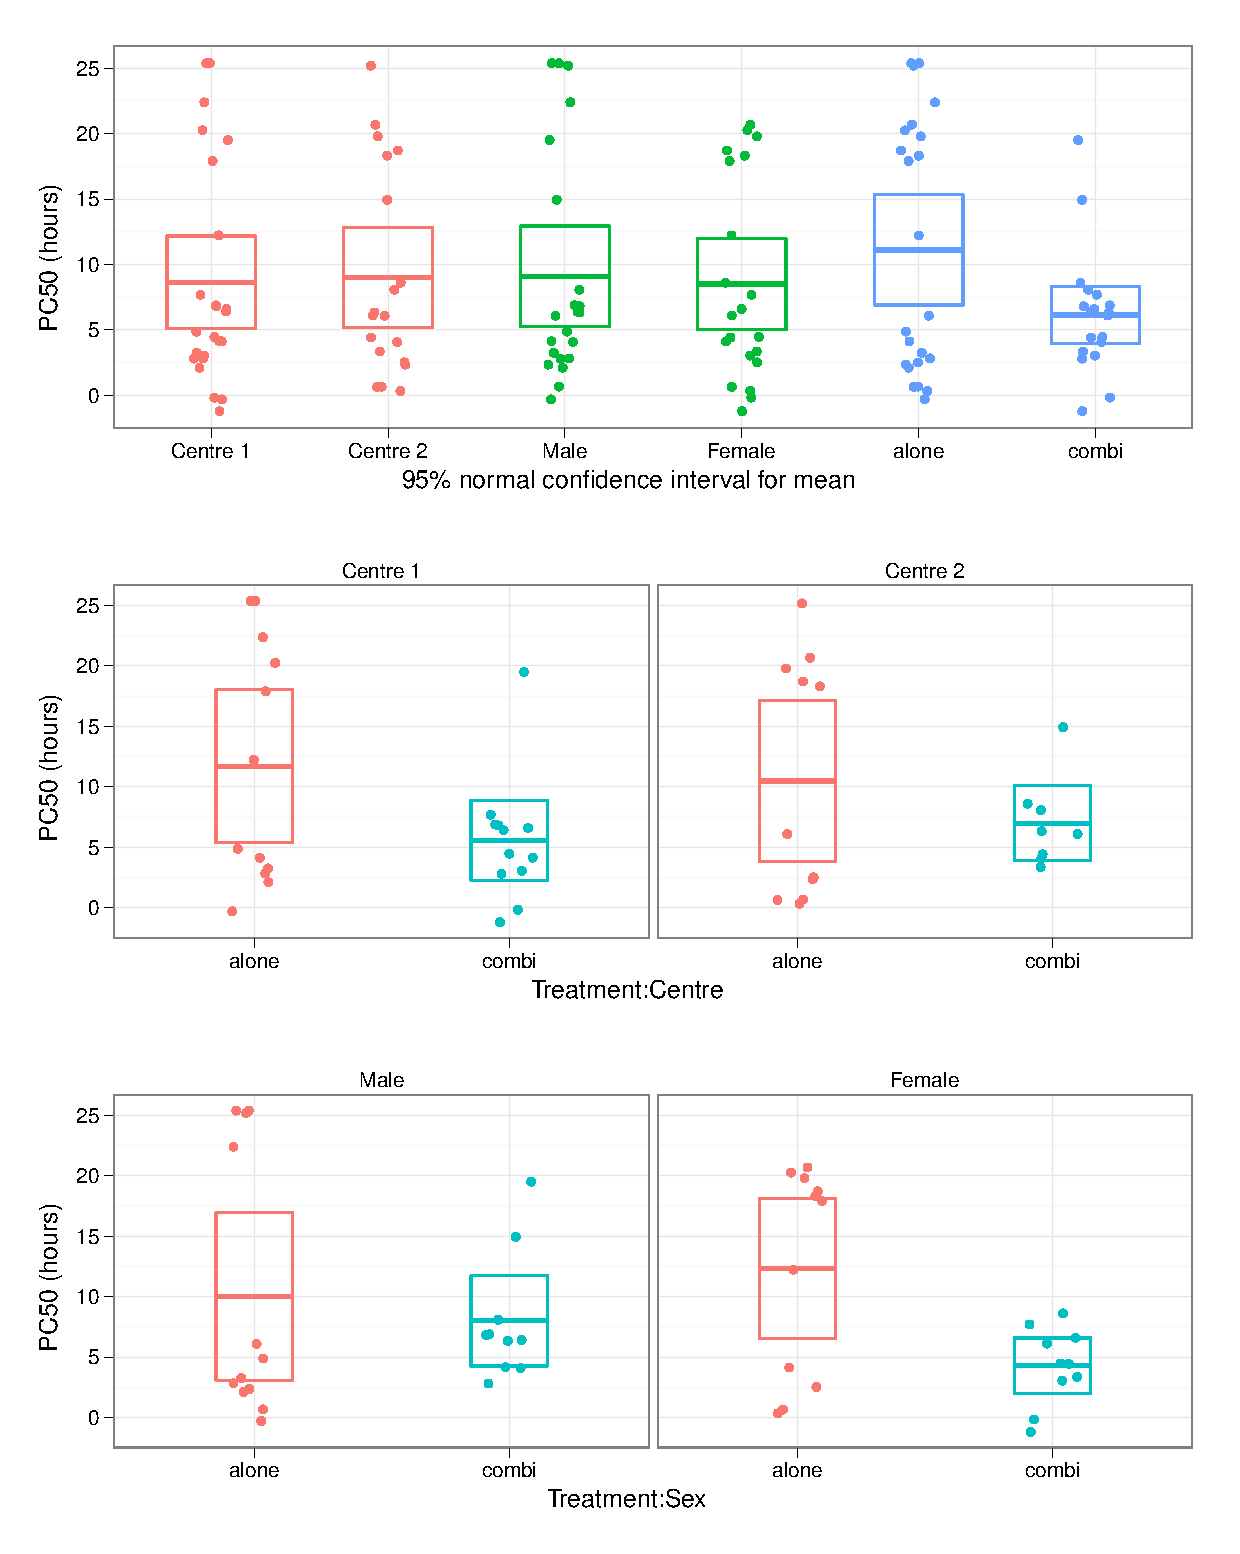
\includegraphics[width=150mm]{pc50anova.eps} 
\caption{Comparison of PC50 main effects and interactions with $t$ distribution 95\% confidence intervals for the means}
\label{pc50anova}
\end{figure}
A similar pattern can be seen as for PC90 (Figures \ref{pc90boxes} and \ref{pc90interaction} on pages \pageref{pc90boxes} and \pageref{pc90interaction}). The same key features are present namely
\begin{itemize}
\item No difference between centres.
\item A reduction in clearance time with the combined treatment, but only for female subjects.
\item A greater variance for subjects on the single (``alone'') treatment.
\end{itemize}

The same procedure of inspecting the distribution of standardized residuals was followed for choosing an appropriate ANOVA model for the data. As with PC90 it was found that the most suitable model for the PC50 clearance time was a 2-way ANOVA model by sex and treatment with a square-root transformation of the dependent variable, fitted by weighted least-squares, using the variances of the two treatment groups as the weighting. The results are shown in Table \ref{aov50}.
%> summary(PC50.loglin2rwt.aov)
%              Df Sum Sq Mean Sq F value  Pr(>F)  
%Sex            1  1.104   1.104  1.1652 0.28702  
%Treatment      1  2.089   2.089  2.2055 0.14556  
%Sex:Treatment  1  3.010   3.010  3.1771 0.08246 .
%Residuals     39 36.949   0.947
\begin{table}[h]
\centering
\caption{ANOVA table for PC50 model}\label{aov50}
\begin{tabular}{l|rrrrrl}
Source&Sum Sq.&df&Mean Sq.&$F$&P($>F$)\\
\hline
$Sex$				& 1.10 & 1 & 1.10 & 1.17 & 0.287 & \\
$Treatment$			& 2.09   & 1 & 2.09   & 2.21   & 0.146 & \\
$Sex\times Treatment$	& 3.01   & 1 & 3.01   & 3.18   & 0.082 & \\
$Residuals$			& 36.95 & 39 & 0.947 &&&\\
\hline
Total&43.15&42&&&
\end{tabular}
\end{table}

Although Figure \ref{pc50anova} seems to show a sex-treatment interaction effect on clearance times we do not have evidence at the 5\% level to reject the hypothesis that there is no effect of sex or treatment. This is probably because the difference between clearance times is smaller than for PC90 and we don't have enough data to detect this difference at the 5\% level.

The mean PC50 clearance times and confidence intervals are shown in Table \ref{inference50}.
\begin{table}[h]
\centering
\caption{Mean PC50 clearance times by sex and treatment}\label{inference50}
\begin{tabular}{|l|c|c|}
\hline
&Clearance time PC50&95\% conf. int.\\
Factor levels&(hrs:mins)&(hrs:mins)\\
\hline
Male, single treatment 		& 6:47 & (2:37, 12:54) \\
Female, single treatment		& 10:02 & (4:34,  17:37) \\
Male, combined treatment	& 7:22 & (3:50, 12:03) \\
Female, combined treatment	& 2:54 & (0:54, 6:03) \\
\hline
\end{tabular}
\end{table}

For female subjects the mean decrease in PC50 in the combined treatment group over the single treatment group is 7.1 hours with a 95\% confidence interval of (0.7, 9.9) hours.

\subsubsection*{PC99}
The log-linear interpolated PC99 values are plotted in Figure \ref{pc99anova}.
\begin{figure}[p]
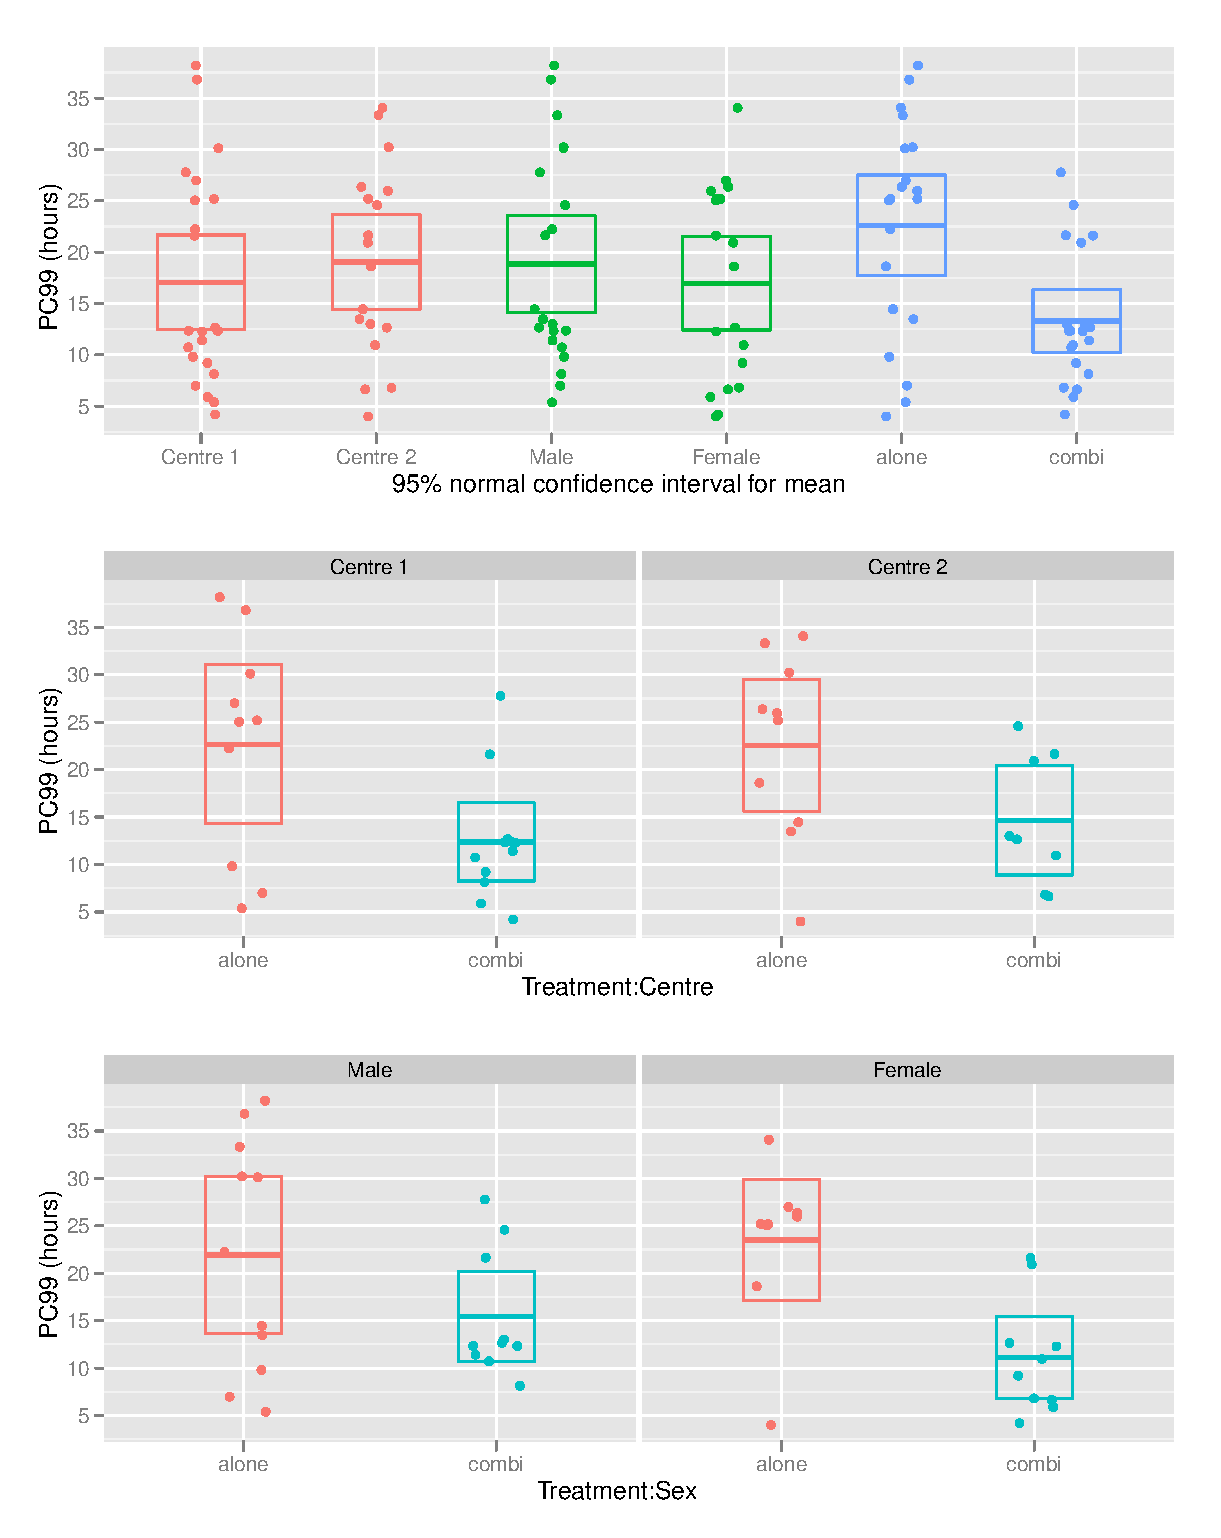
\includegraphics[width=150mm]{pc99anova.eps} 
\caption{Comparison of PC99 main effects and interactions with $t$ distribution 95\% confidence intervals for the means}
\label{pc99anova}
\end{figure}
For 3 subjects the parasite count did not reach the PC99 level by the end of the study, hence there is only PC99 data for 40 out of the 43 subjects. Once again there is no discernible effect of centre or sex alone on the clearance times. However, now the improvement of the combined treatment over the single treatment seems more symmetrical between sexes. Results of 2-way ANOVA by sex and treatment on the square-root transformed clearance times fitted by treatment-weighted least-squares are shown in Table \ref{aov99}.
%              Df Sum Sq Mean Sq F value   Pr(>F)   
%Sex            1  1.436   1.436  1.4664 0.233808   
%Treatment      1  9.074   9.074  9.2688 0.004339 **
%Sex:Treatment  1  1.643   1.643  1.6781 0.203416   
%Residuals     36 35.243   0.979              
\begin{table}[h]
\centering
\caption{ANOVA table for PC99 model}\label{aov99}
\begin{tabular}{l|rrrrrl}
Source&Sum Sq.&df&Mean Sq.&$F$&P($>F$)\\
\hline
$Sex$				& 1.44 & 1 & 1.44 & 1.47 & 0.234 & \\
$Treatment$			& 9.07   & 1 & 9.07   & 9.27   & 0.004 &** \\
$Sex\times Treatment$	& 1.64   & 1 & 1.64   & 1.68   & 0.203 & \\
$Residuals$			& 35.243 & 36 & 0.979 &&&\\
\hline
Total&47.40&39&&&
\end{tabular}\\
**$<0.005$
\end{table}

It can be seen that there is evidence to reject the hypothesis that treatment has no effect on PC99 clearance time, but no evidence to reject the hypothesis that sex has no effect. Therefore, we can exclude sex as a factor and refit a 1-way ANOVA model by treatment alone, giving the results shown in Table \ref{aov99r}.
%            Df Sum Sq Mean Sq F value  Pr(>F)   
%Treatment    1  9.396   9.396  9.3959 0.00399 **
%Residuals   38 38.000   1.000   
\begin{table}[h]
\centering
\caption{1-way ANOVA table for PC99 model}\label{aov99r}
\begin{tabular}{l|rrrrrl}
Source&Sum Sq.&df&Mean Sq.&$F$&P($>F$)\\
\hline
$Treatment$			& 9.40   & 1 & 9.40   & 9.40   & 0.004 &** \\
$Residuals$			& 38.0 & 38 & 1.00 &&&\\
\hline
Total&47.40&39&&&
\end{tabular}\\
**$<0.005$
\end{table}

The mean PC99 clearance time for patients on the single treatment is 21:07 (hrs:mins) with a 95\% confidence interval of (16:12, 26:41); for the combined treatment it is 12:33 (9:53, 15:32). This gives a mean decrease in PC99 for subjects on the combined treatment over the single treatment of 9.3 hours with a 95\% confidence interval of (3.7, 15.0) hours.

\subsection{Parasite reduction ratios}
Another endpoint used in studies of the efficacy of antimalarial drugs is the \emph{Parasite Reduction Ratio}, which is the ratio of the pre-dose parasite count to the count at a specific time from the time of first dose. 48 hours is often chosen as a time to calculate this ratio (PRR48) as this represents the reduction in parasites over a single lifecycle of the parasites\cite{white}. ``PRR24'', The reduction over 24 hours is also used\cite{newton}.

PRR48 measurements are not available for our data as the parasite count is 0 by 48 hours for all but 6 subjects. Even after 24 hours there are only 25 of the 43 subjects with non-zero parasite counts. After 12 hours though there are still 37 of the 43 subjects with a non-zero parasite count so we can look at PRR12 and have reasonable numbers in groups to make comparisons between treatments. The log parasite reduction ratio after 12 hours is shown in Figure \ref{prr12}
\begin{figure}
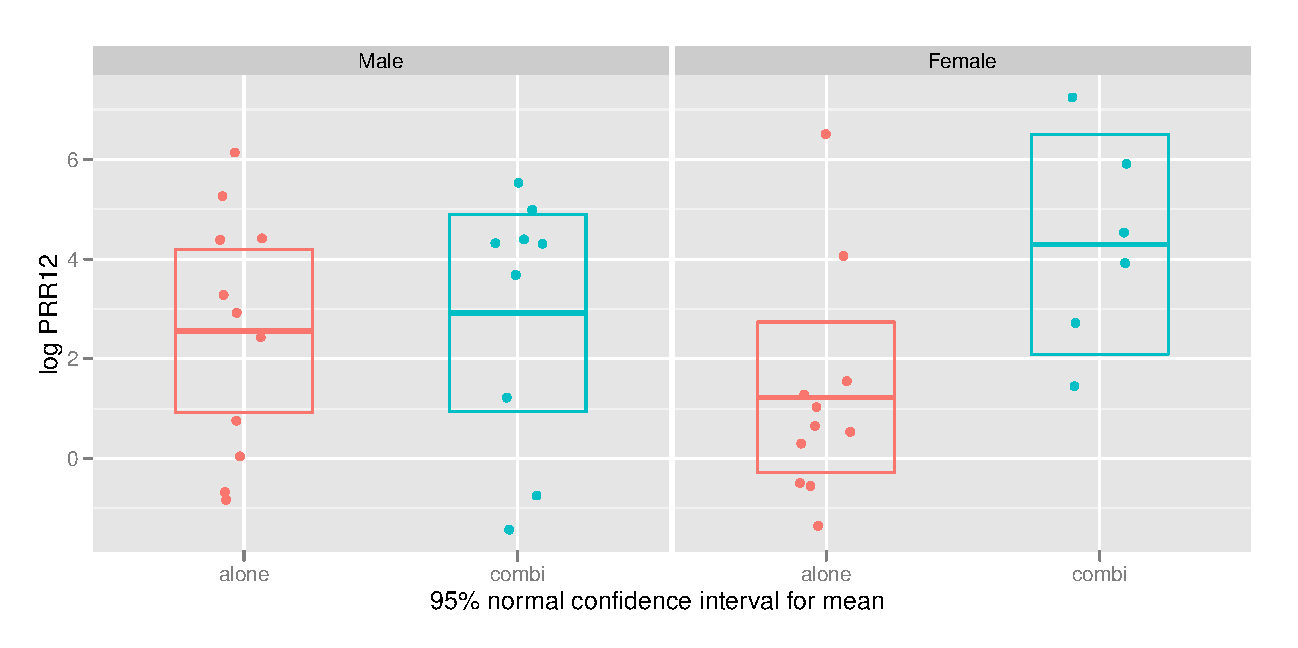
\includegraphics[width=150mm]{prr12.eps} 
\caption{log PRR12 with 95\% confidence intervals for the means}
\label{prr12}
\end{figure}

A similar pattern as with the PC90 and PC50 endpoints can be seen in that the treatment only seems to be effective among female patients in increasing PRR. It was found that a logarithmic transformation was appropriate for 2-way ANOVA modelling of the PRR12 data giving the results shown in Table \ref{aovprr12}.
%              Df  Sum Sq Mean Sq F value  Pr(>F)  
%Sex            1   1.524   1.524  0.2725 0.60512  
%Treatment      1  21.265  21.265  3.8024 0.05972 .
%Sex:Treatment  1  15.951  15.951  2.8521 0.10069  
%Residuals     33 184.557   5.593          
\begin{table}[h]
\centering
\caption{ANOVA table for PC99 model}\label{aovprr12}
\begin{tabular}{l|rrrrrl}
Source&Sum Sq.&df&Mean Sq.&$F$&P($>F$)\\
\hline
$Sex$				& 1.52 & 1 & 1.52 & 0.273 & 0.605 & \\
$Treatment$			& 21.27   & 1 & 21.27   & 3.80 & 0.060 & \\
$Sex\times Treatment$	& 15.95   & 1 & 15.95   & 2.85   & 0.101 & \\
$Residuals$			& 184.56 & 33 & 5.59 &&&\\
\hline
Total&223.30&36&&&
\end{tabular}
\end{table}

It can be seen that there is some evidence between the 5 and 10\% level to reject the hypothesis that the treatment has no effect on the parasite reduction ratio after 12 hours. It may be that we don't have enough data to detect the treatment effect observed in Figure \ref{prr12}. The model gives a mean increase in PRR12 for subjects on the combined treatment over those on the single treatment of 25.5 with a 95\% confidence interval of (-0.4, 159.8).

%\subsection{Logistic model of those cured after 24 hours?}

\section{Functional data analysis}
\subsection{Overview of functional data analysis}
Functional data analysis(FDA) is a relatively new technique whereby the data is analysed in terms of smooth functions. An example is longitudinal data such as the growth of children or the weather over a year\cite{ramsay}. With such data we describe the response with a smooth function and then look at the ways the characteristics of the function change between cases. This type of analysis can make use of looking at derivitives of the functions to look for patterns in rates of change. Functional data analysis is somewhat analagous to multivariate data analysis, looking at multiple responses and characteristic combinations of responses between \emph{replicates}.

The parasite count data in this study is a good candidate for functional data analysis in that the response for each replicate of experimental factors centre, sex and treatment can be described as a smooth function of parasite count with time. We already used cubic and logistic functions in order to extract a single response variable, the PC90 clearance time, but now we can go on to explore the nature of a functional response.

Many familiar statistical summaries and techniques have functional equivalents. Means and standard deviations can be expressed as mean functions and standard deviation functions for example. Regression and ANOVA can be performed with functional dependent and independent variables yielding coefficient functions and residual functions.
\subsection{Basis functions}
The first step in FDA is to identify an appropriate smoothing function for our data known as a \emph{basis function}. For periodic data fourier functions are normally used, for non-periodic data the most commonly used basis functions are cubic splines\cite{fda}. Fitting a cubic spline requires choice of \emph{breakpoints} or ``knots'' (not entirely interchangeable terms) between which we fit cubic polynomials. The simplest choice of breakpoints with longitudinal data is to choose the times at which the data were taken. We also specify a smoothness parameter that limits the size of higher derivitives and hence the sharpness of the curve.


\begin{figure}[h]
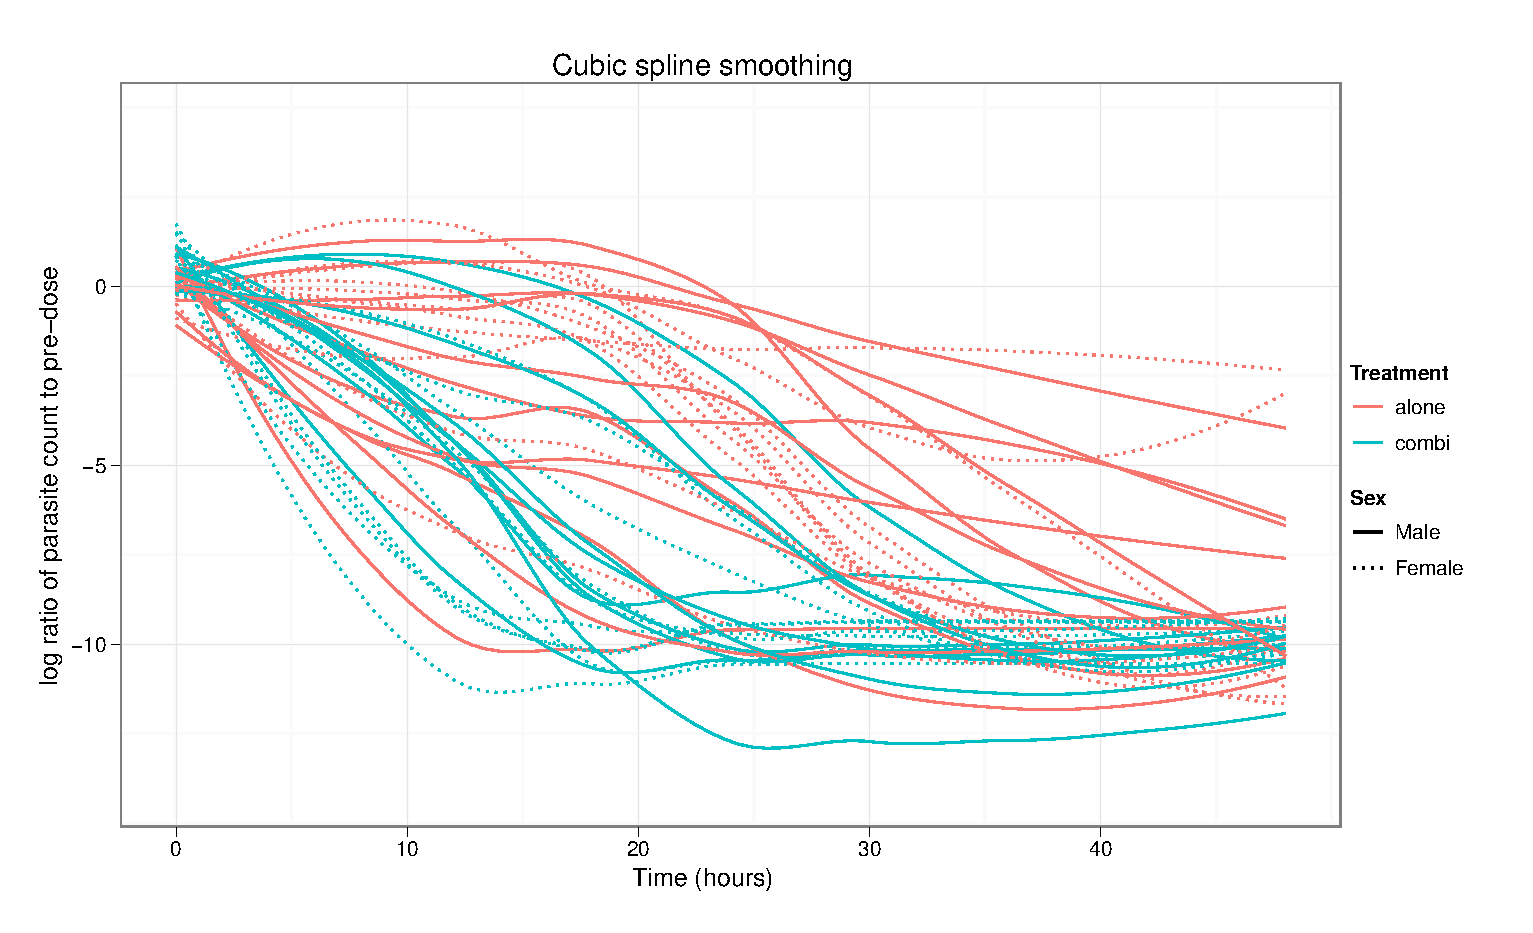
\includegraphics[width=150mm]{cubicspline.eps} 
\caption{}
\label{cubicspline}
\end{figure}
\begin{figure}[h]
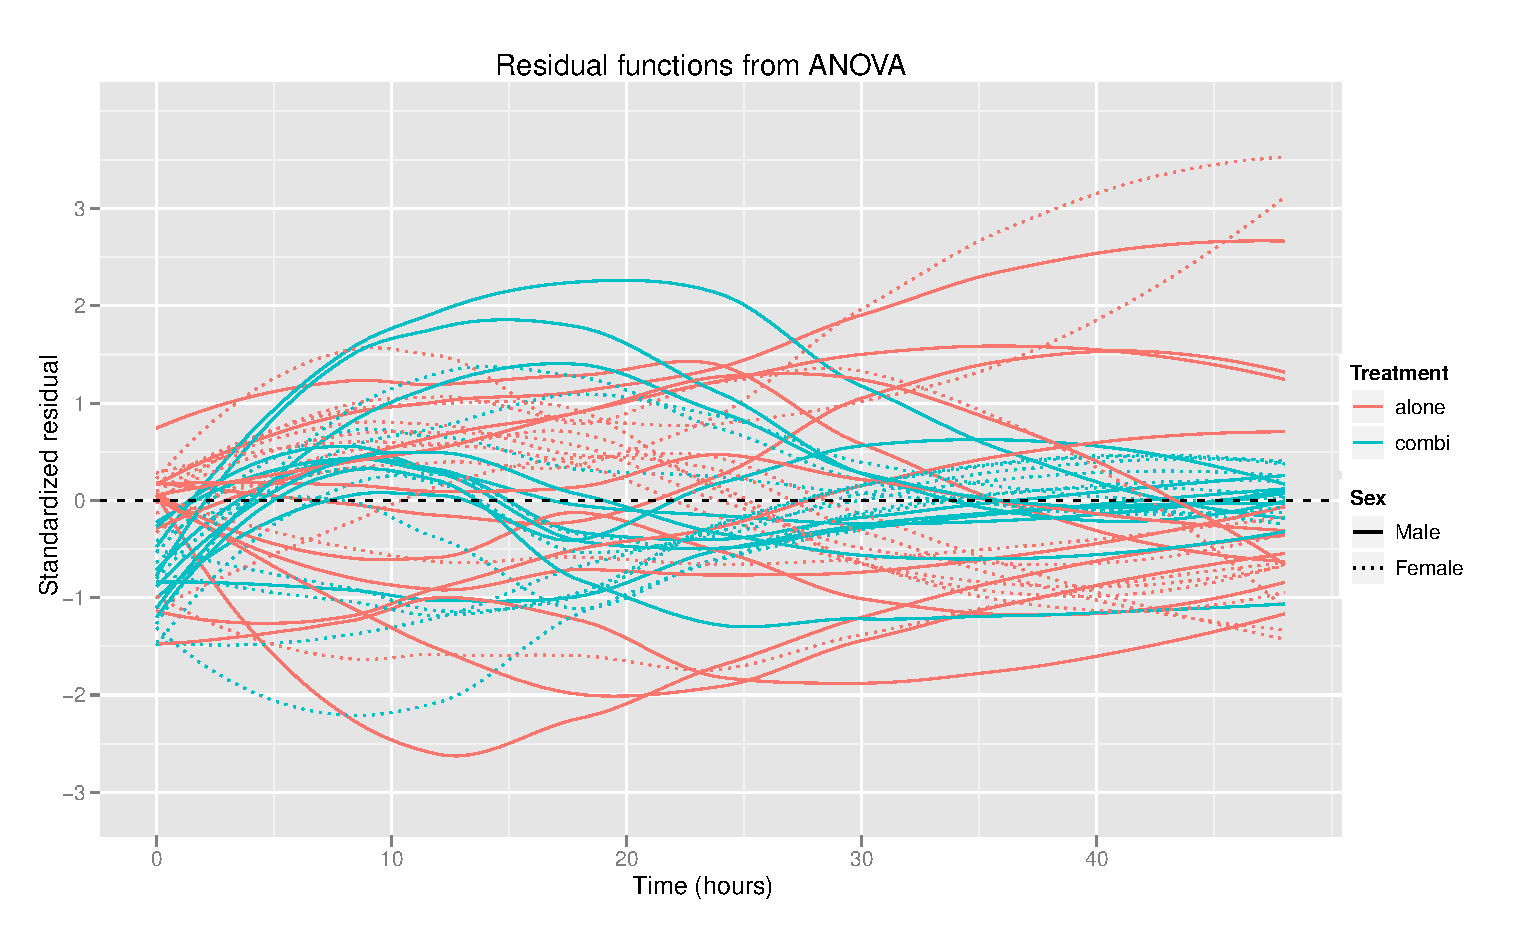
\includegraphics[width=150mm]{fdaresids.eps} 
\caption{}
\label{fdaresids}
\end{figure}
\begin{figure}[h]
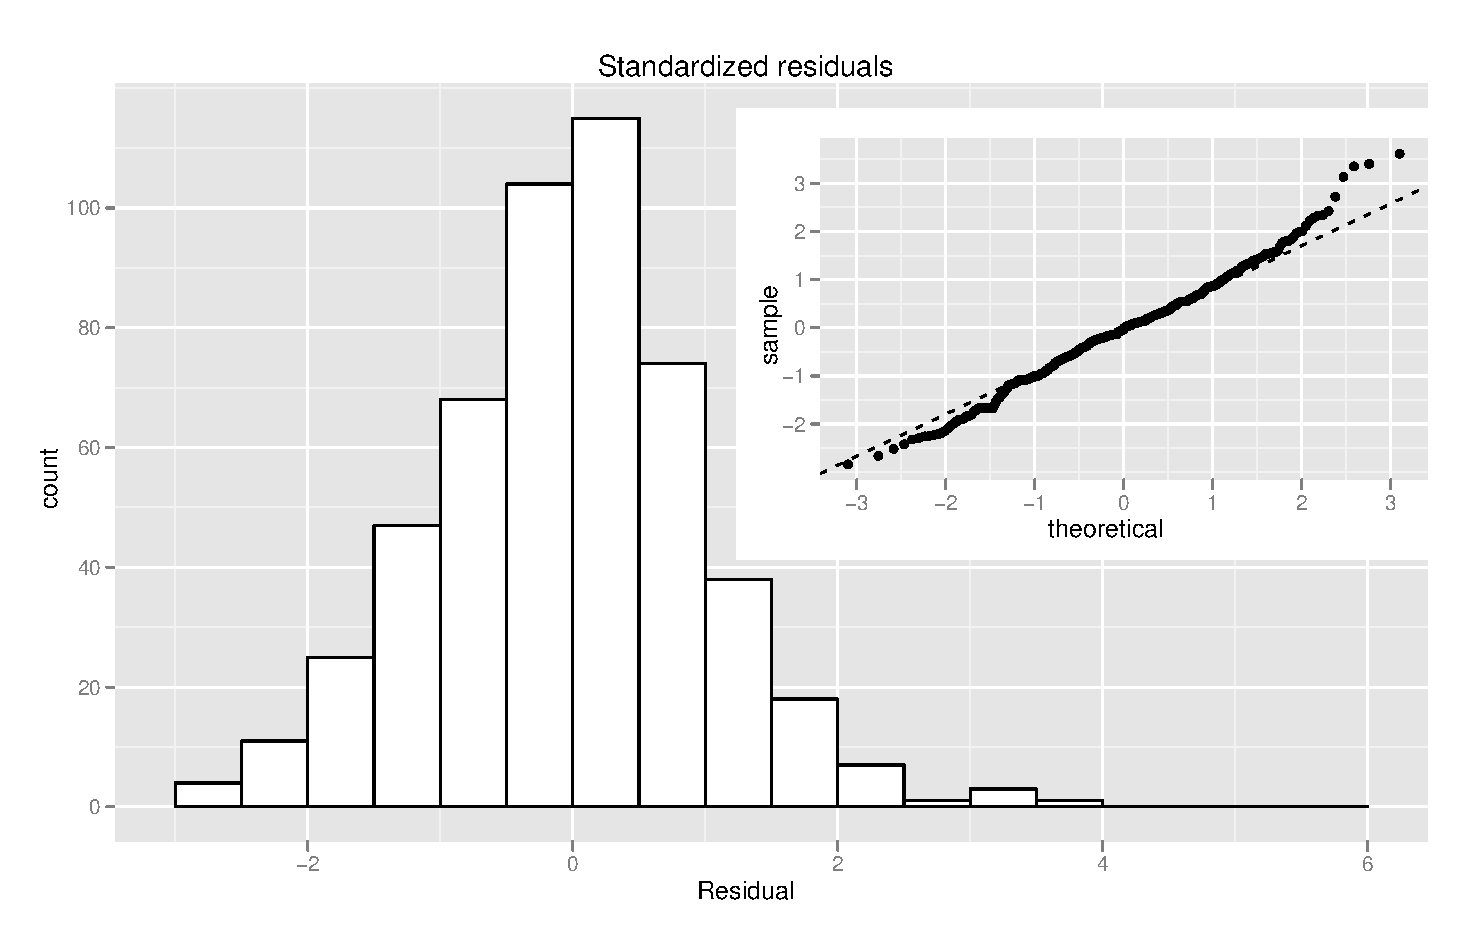
\includegraphics[width=150mm]{fdahistqq.eps} 
\caption{}
\label{fdahistqq}
\end{figure}
\begin{figure}[h]
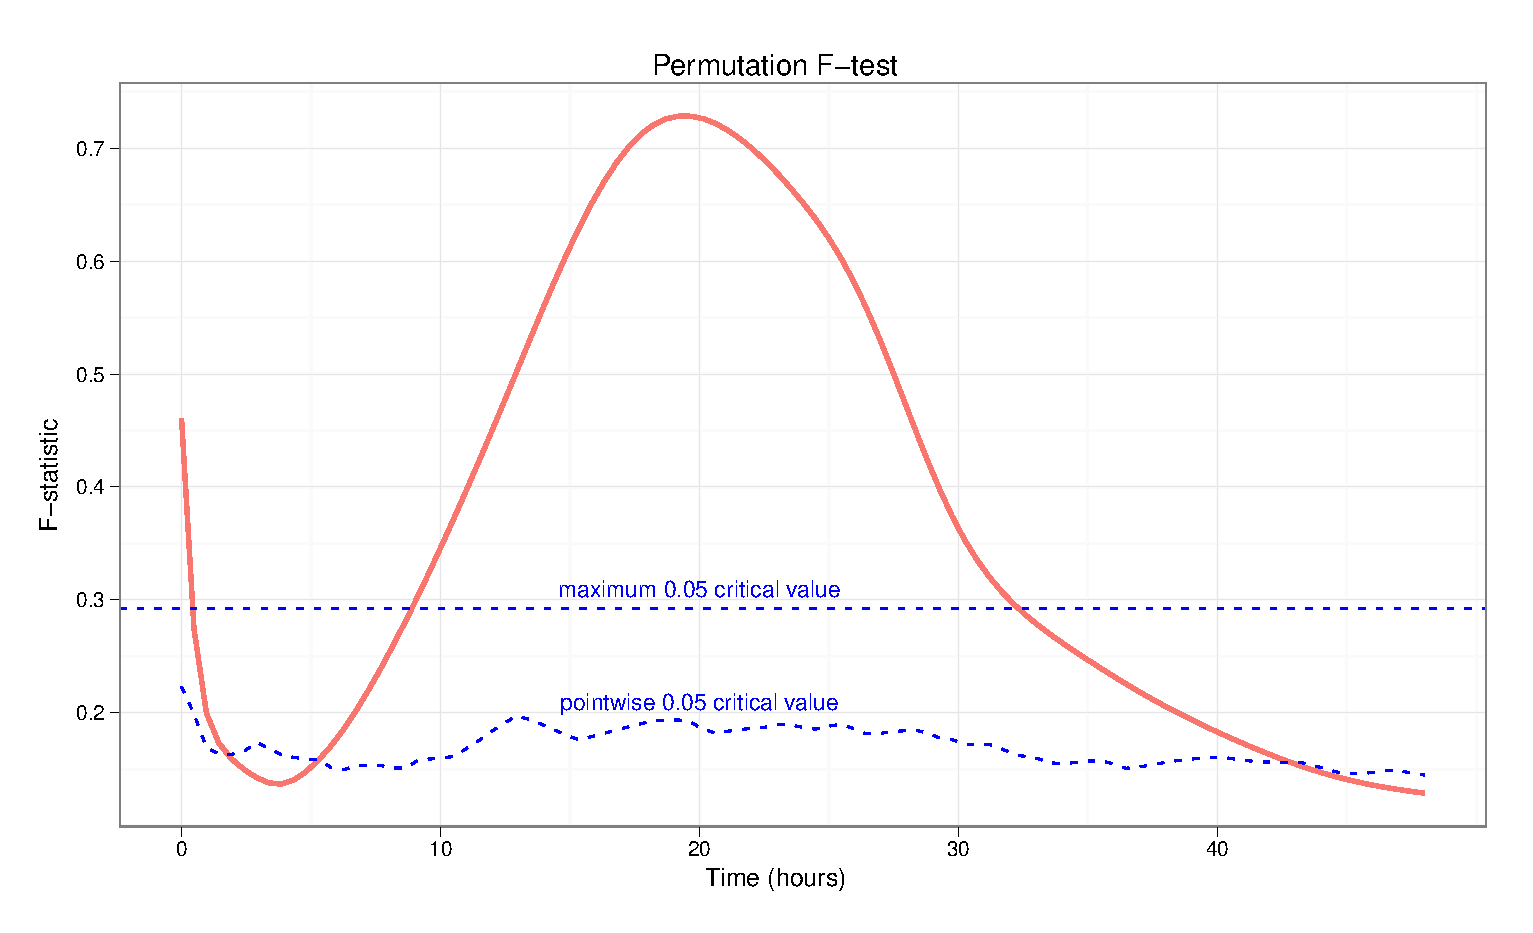
\includegraphics[width=150mm]{fdapermF.eps} 
\caption{}
\label{fdapermF}
\end{figure}
\begin{figure}[h]
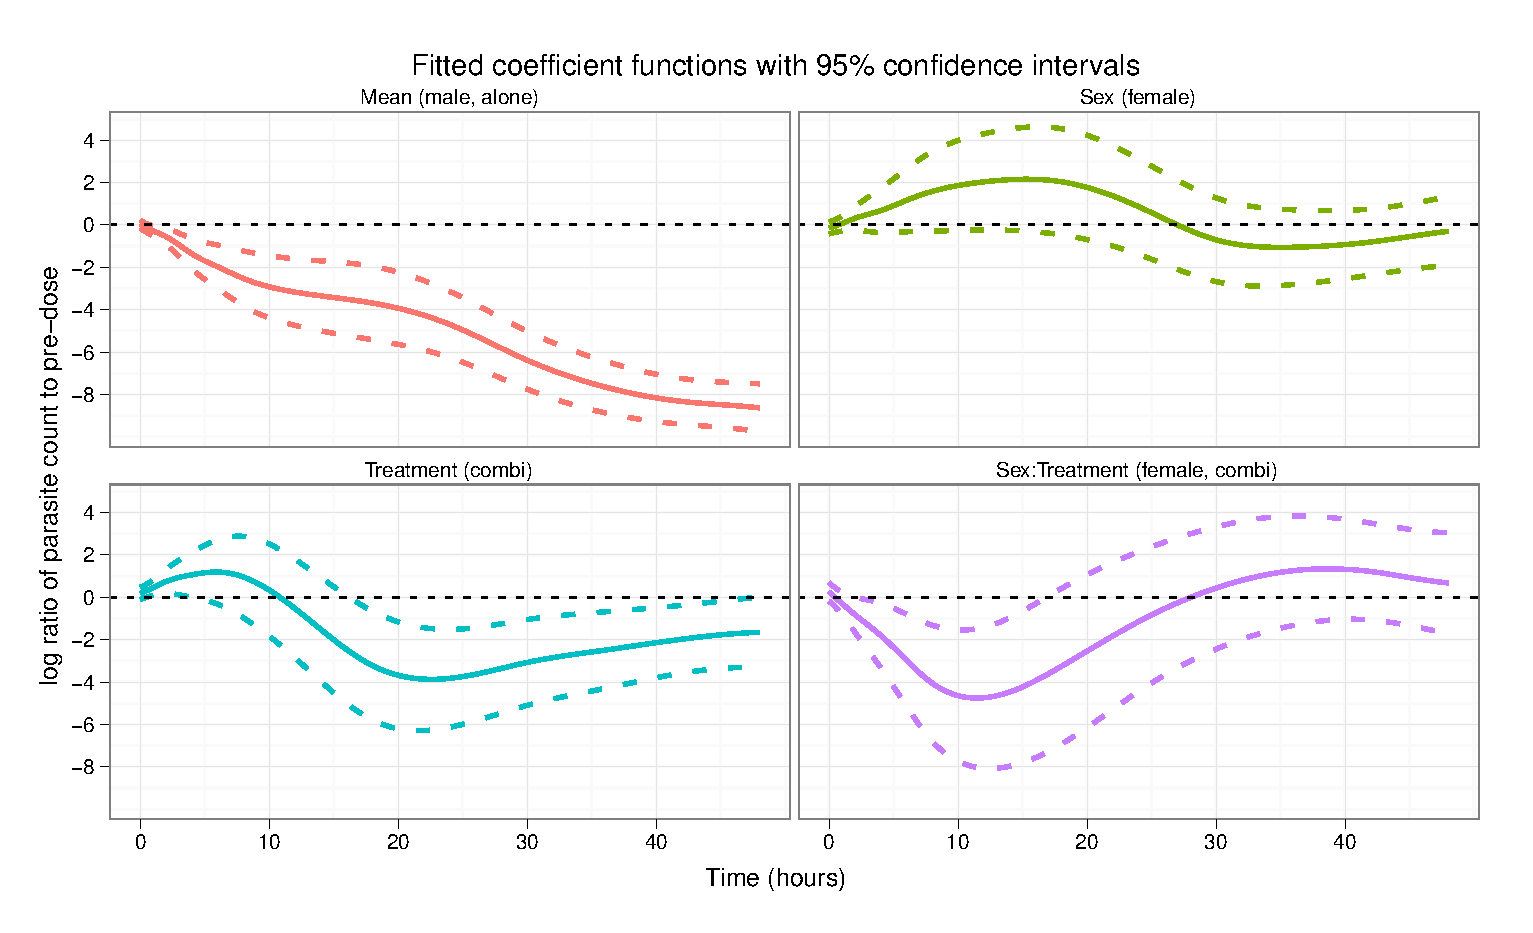
\includegraphics[width=150mm]{fdcoef.eps} 
\caption{}
\label{fdcoef}
\end{figure}
\begin{figure}[h]
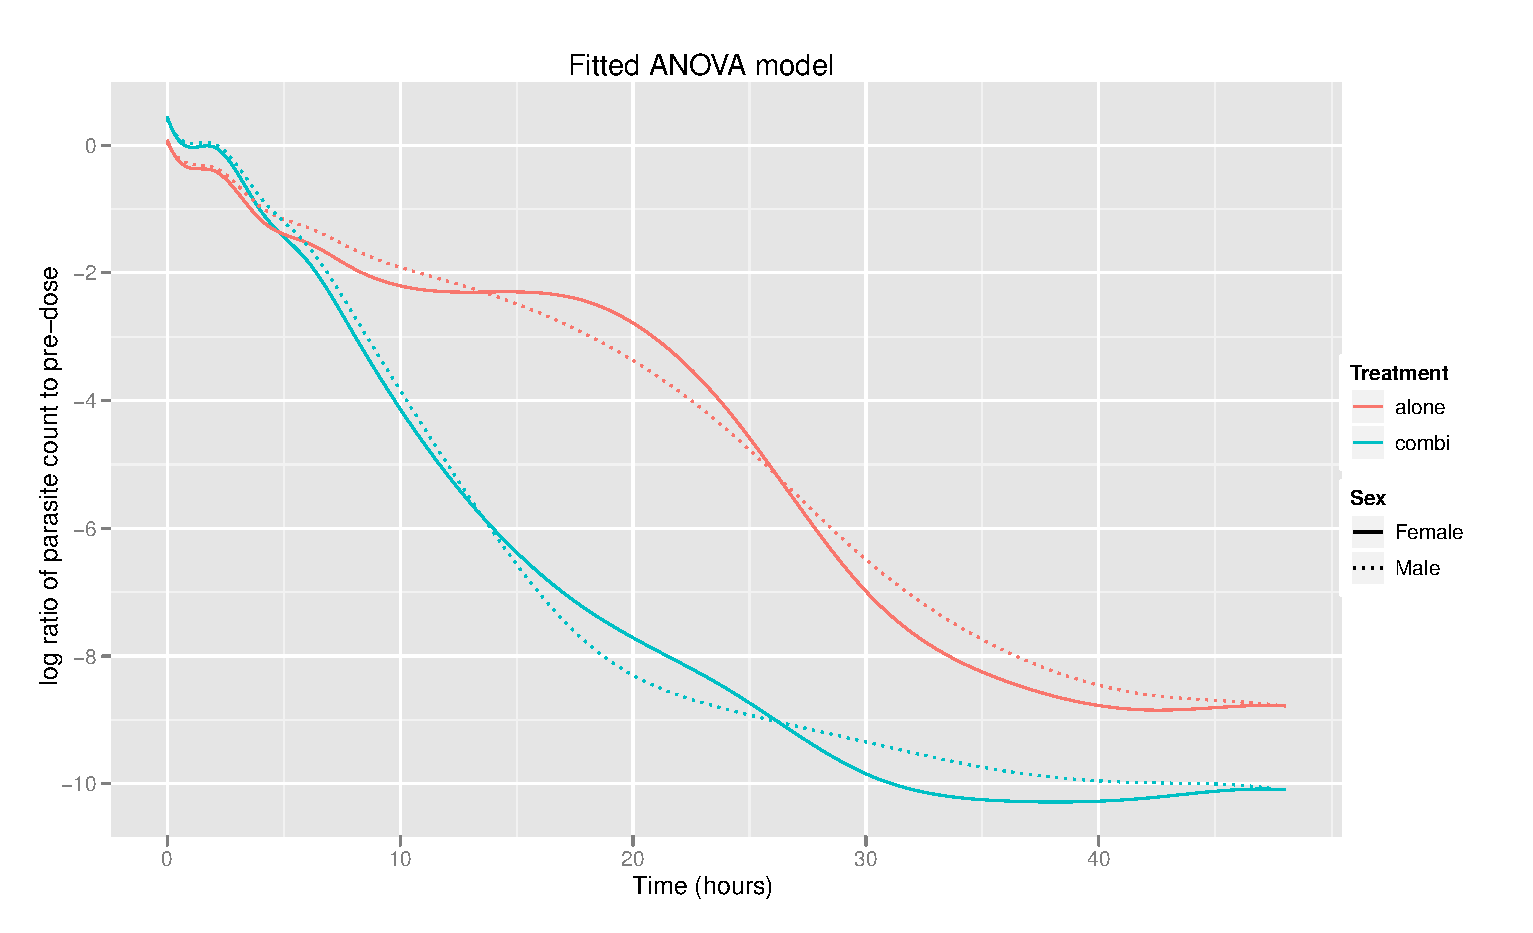
\includegraphics[width=150mm]{fdfitted.eps} 
\caption{}
\label{fdfitted}
\end{figure}

%\section{Key results}
\chapter{Discussion}\label{ch:discussion}
The were two primary questions addressed in this dissertation.
\begin{enumerate}
\item Given profiles of parasite counts per microlitre of blood with time from first dose of an antimalarial treatment, how do we derive an estimate of the time taken for 90\% of the parasites to be cleared from the blood?
\item Given our estimated times for parasite clearance, how do we determine if the average clearance time for subjects on one antimalarial treatment is significantly different to the average clearance time for subjects on an alternative treatment?
\end{enumerate}
The first question is not really one that can be formulated as a statistical hypothesis test, but is more a question of making a sensible and consistent estimate. The second question can be answered by the identification of a suitable test statistic.

The following discussion is primarily concerned with how these questions have been answered, but also goes on to look at some of the wider issues raised concerning analysis of data of this type.

\section{Derivation of clearance times}

\subsection{The nature of the problem}
In order to estimate the time for the parasite count to reach 90\% of its pre-dose level we need to know the nature of how the parasite count changes with time. Whether it falls monotonically, for example, follows a linear, or more complicated trend. The observed behaviours were summarised in section \ref{sec:behaviours} and can be seen in Figures \ref{raw1} and \ref{raw2} on pages \pageref{raw1} and \pageref{raw2}. One problem with this data is that we do not know how much of the erratic variation in parasite count per microlitre recorded genuinely reflects a sharp change in the parasite load of the subject and how much is due to error in the counting procedure. It is reported for patients taking antimalarial drugs that ``\textit{parasitemia may rise alarmingly in the hours following treatment}'' \cite{white}. However, it was reported by our contact at GSK that there may be a large variability in parasite counts simply due to the choice of the ``suitable'' area of the blood sample slide chosen by microscopists for parasite counting. Nevertheless, it seems that in the region around the PC90 level that the fall in parasite count is fairly smooth and not nearly as erratic as at earlier times. This can be seen in Figure \ref{comprawlog} on \pageref{comprawlog}. Hence, it seems that estimation between data recording times is more predictable in the PC90 region than at earlier times and that early erratic variation in the count is irrelevant. In this respect PC90 would seem a sensible choice of endpoint.
\subsection{Choice of interpolation method}
\subsubsection*{Criticism of the choice of logistic modelling}
We were told by GSK that logistic modelling had already been used for PC90 estimation for this data and suggested aims for this dissertation were the investigation of the logistic approach such as how to choose appropriate starting parameters for the fitting. This was done, however it was found that the logistic model simply did not have the appropriate shape for modelling the parasite-count profiles of some subjects. It is also not clear as to why a model for the whole count profile must be fitted in order to make an estimate within a narrow time window between observations that bracket the time of interest. It could be argued that the two observations either side of the PC90 time could be subject to a relatively large error and therefore the behaviour should be averaged over a wider timescale. However, this could be more suitably achieved with some sort of spline regression as it seems innappropriate for large fluctuations at early times to influence the estimate at later times when the count profile is relatively smooth.

Some problems with logistic regression are highlighted by Wootton {\it et al.}  

\section{Analysis of clearance times}

{\backmatter
\bibliographystyle{wileyj}
\renewcommand{\bibname}{References}
{\singlespace\bibliography{dissertation}}}
\addappheadtotoc
\appendix
\appendixpage
\chapter{Complete plots of data}
\section{Raw parasite counts}
\begin{sidewaysfigure}
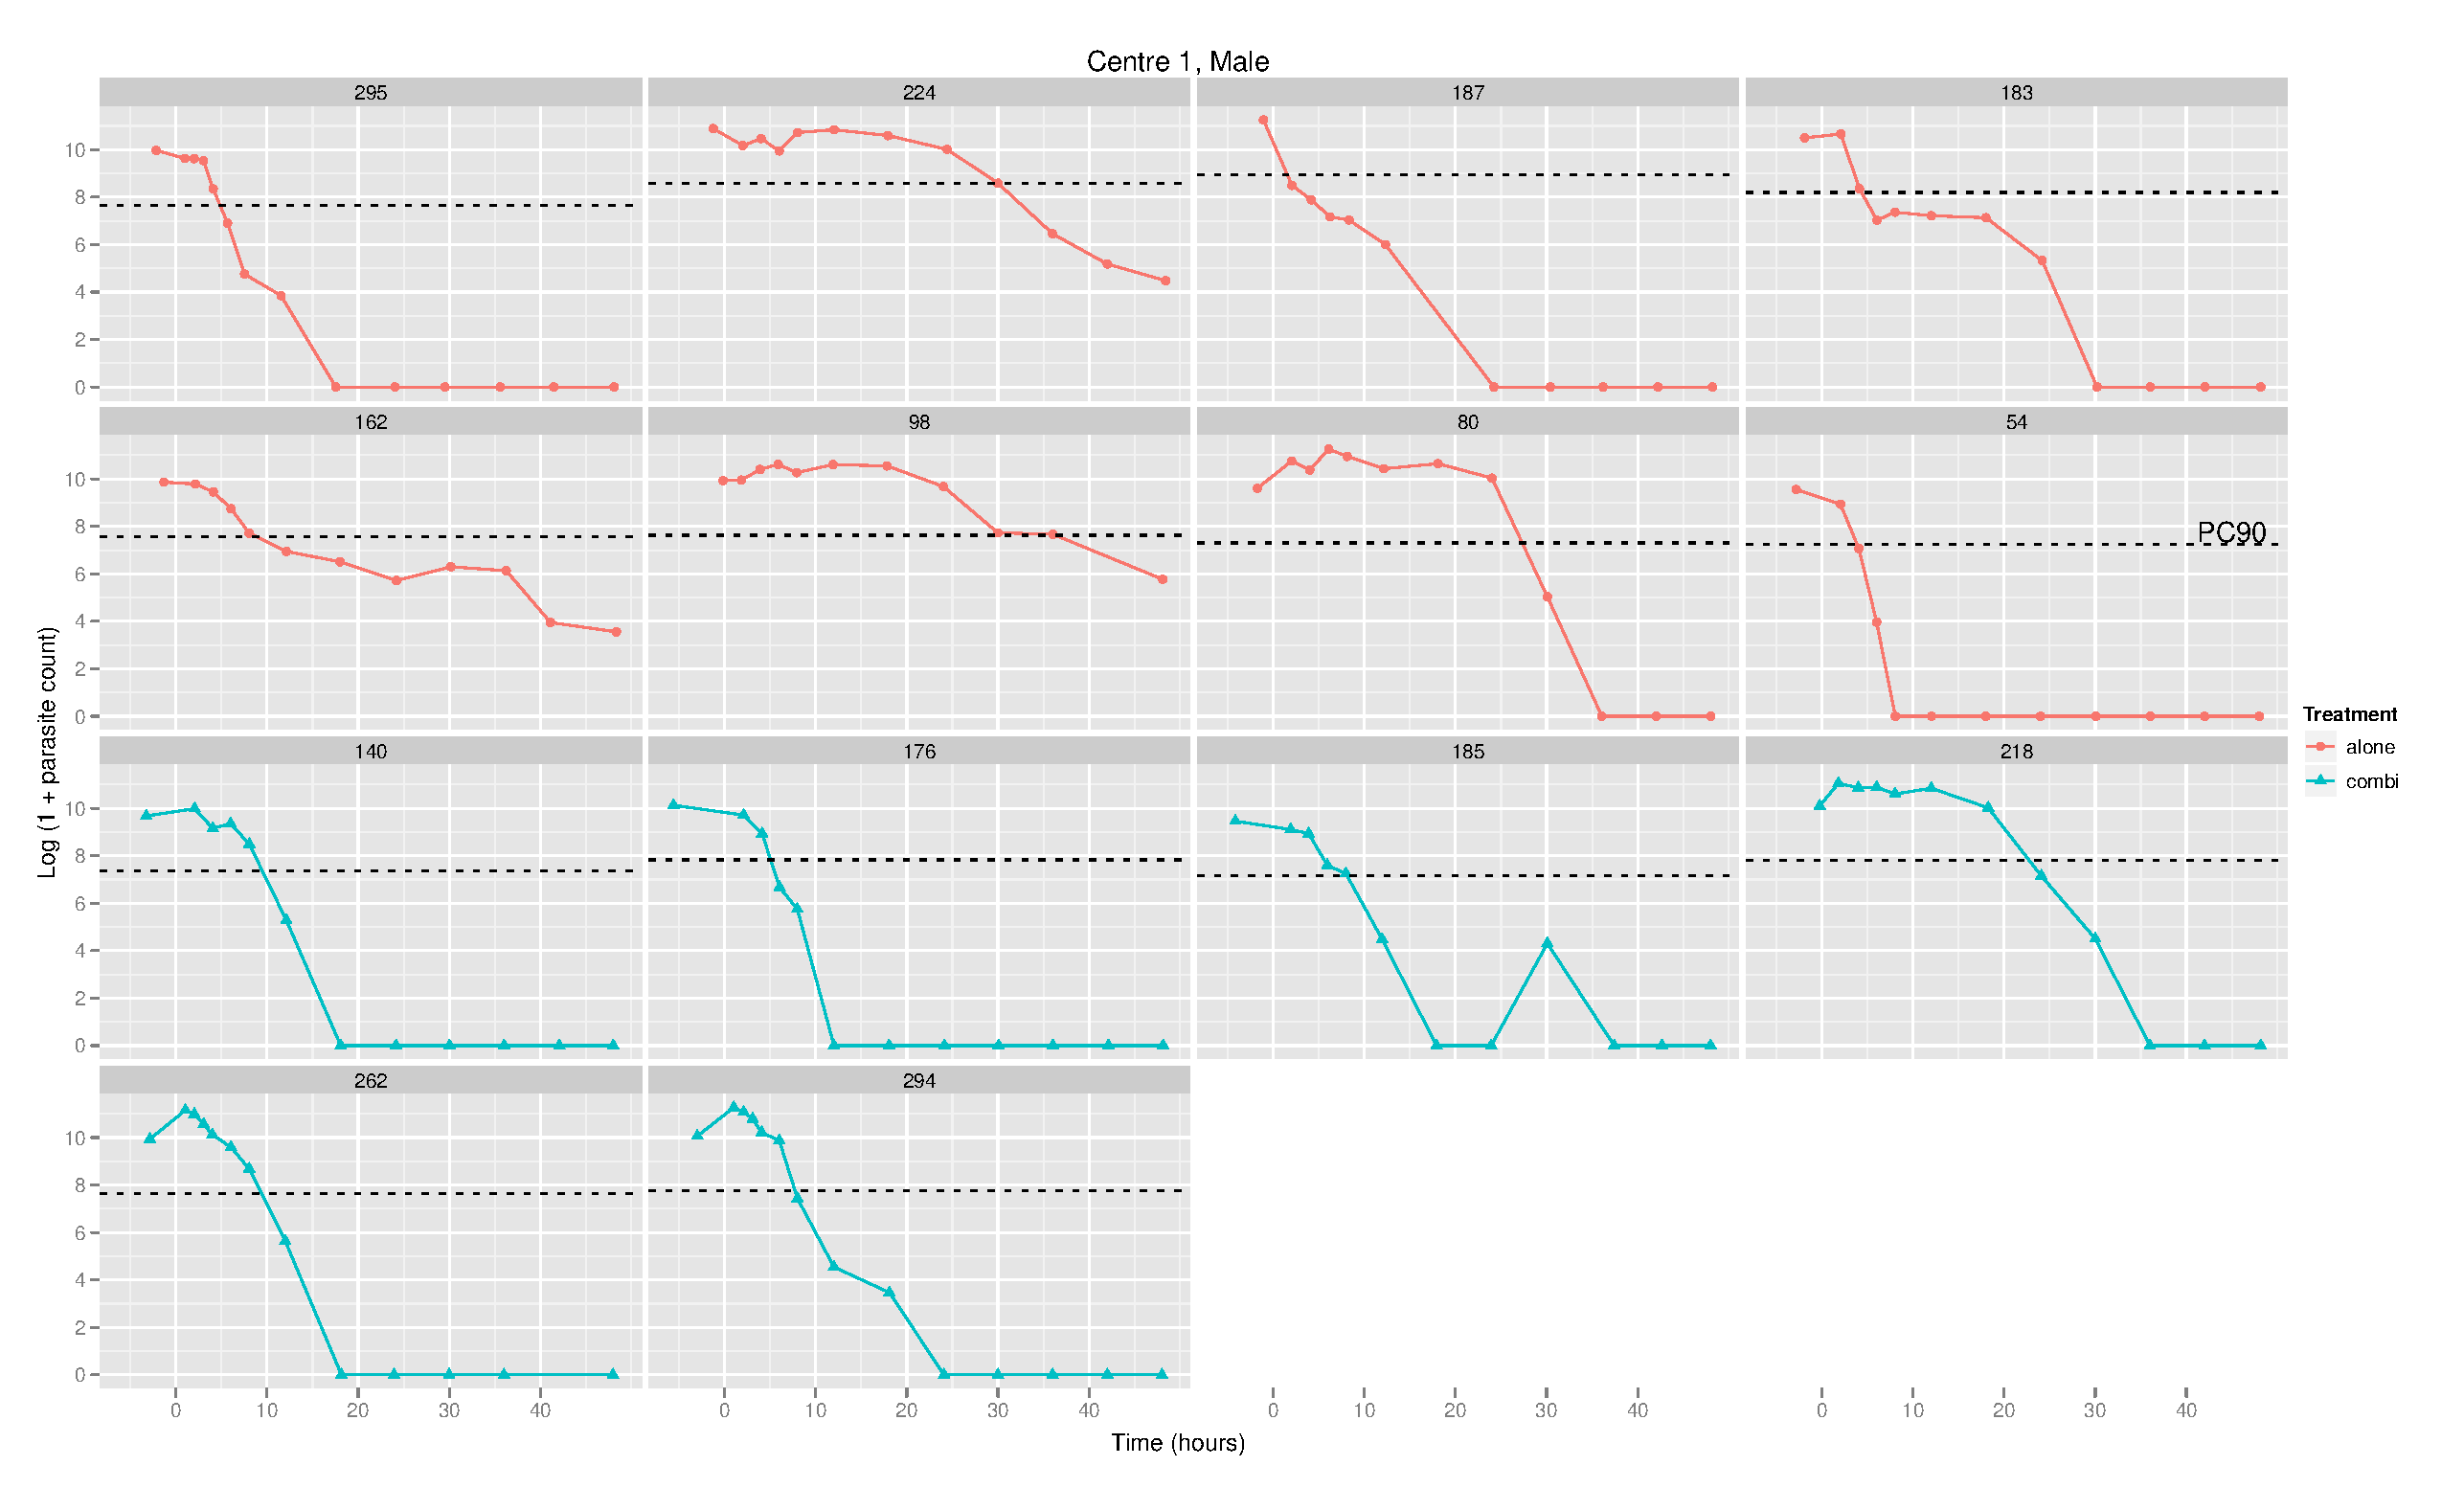
\includegraphics[height=150mm]{Araw1M.eps}
\end{sidewaysfigure}
\begin{sidewaysfigure}
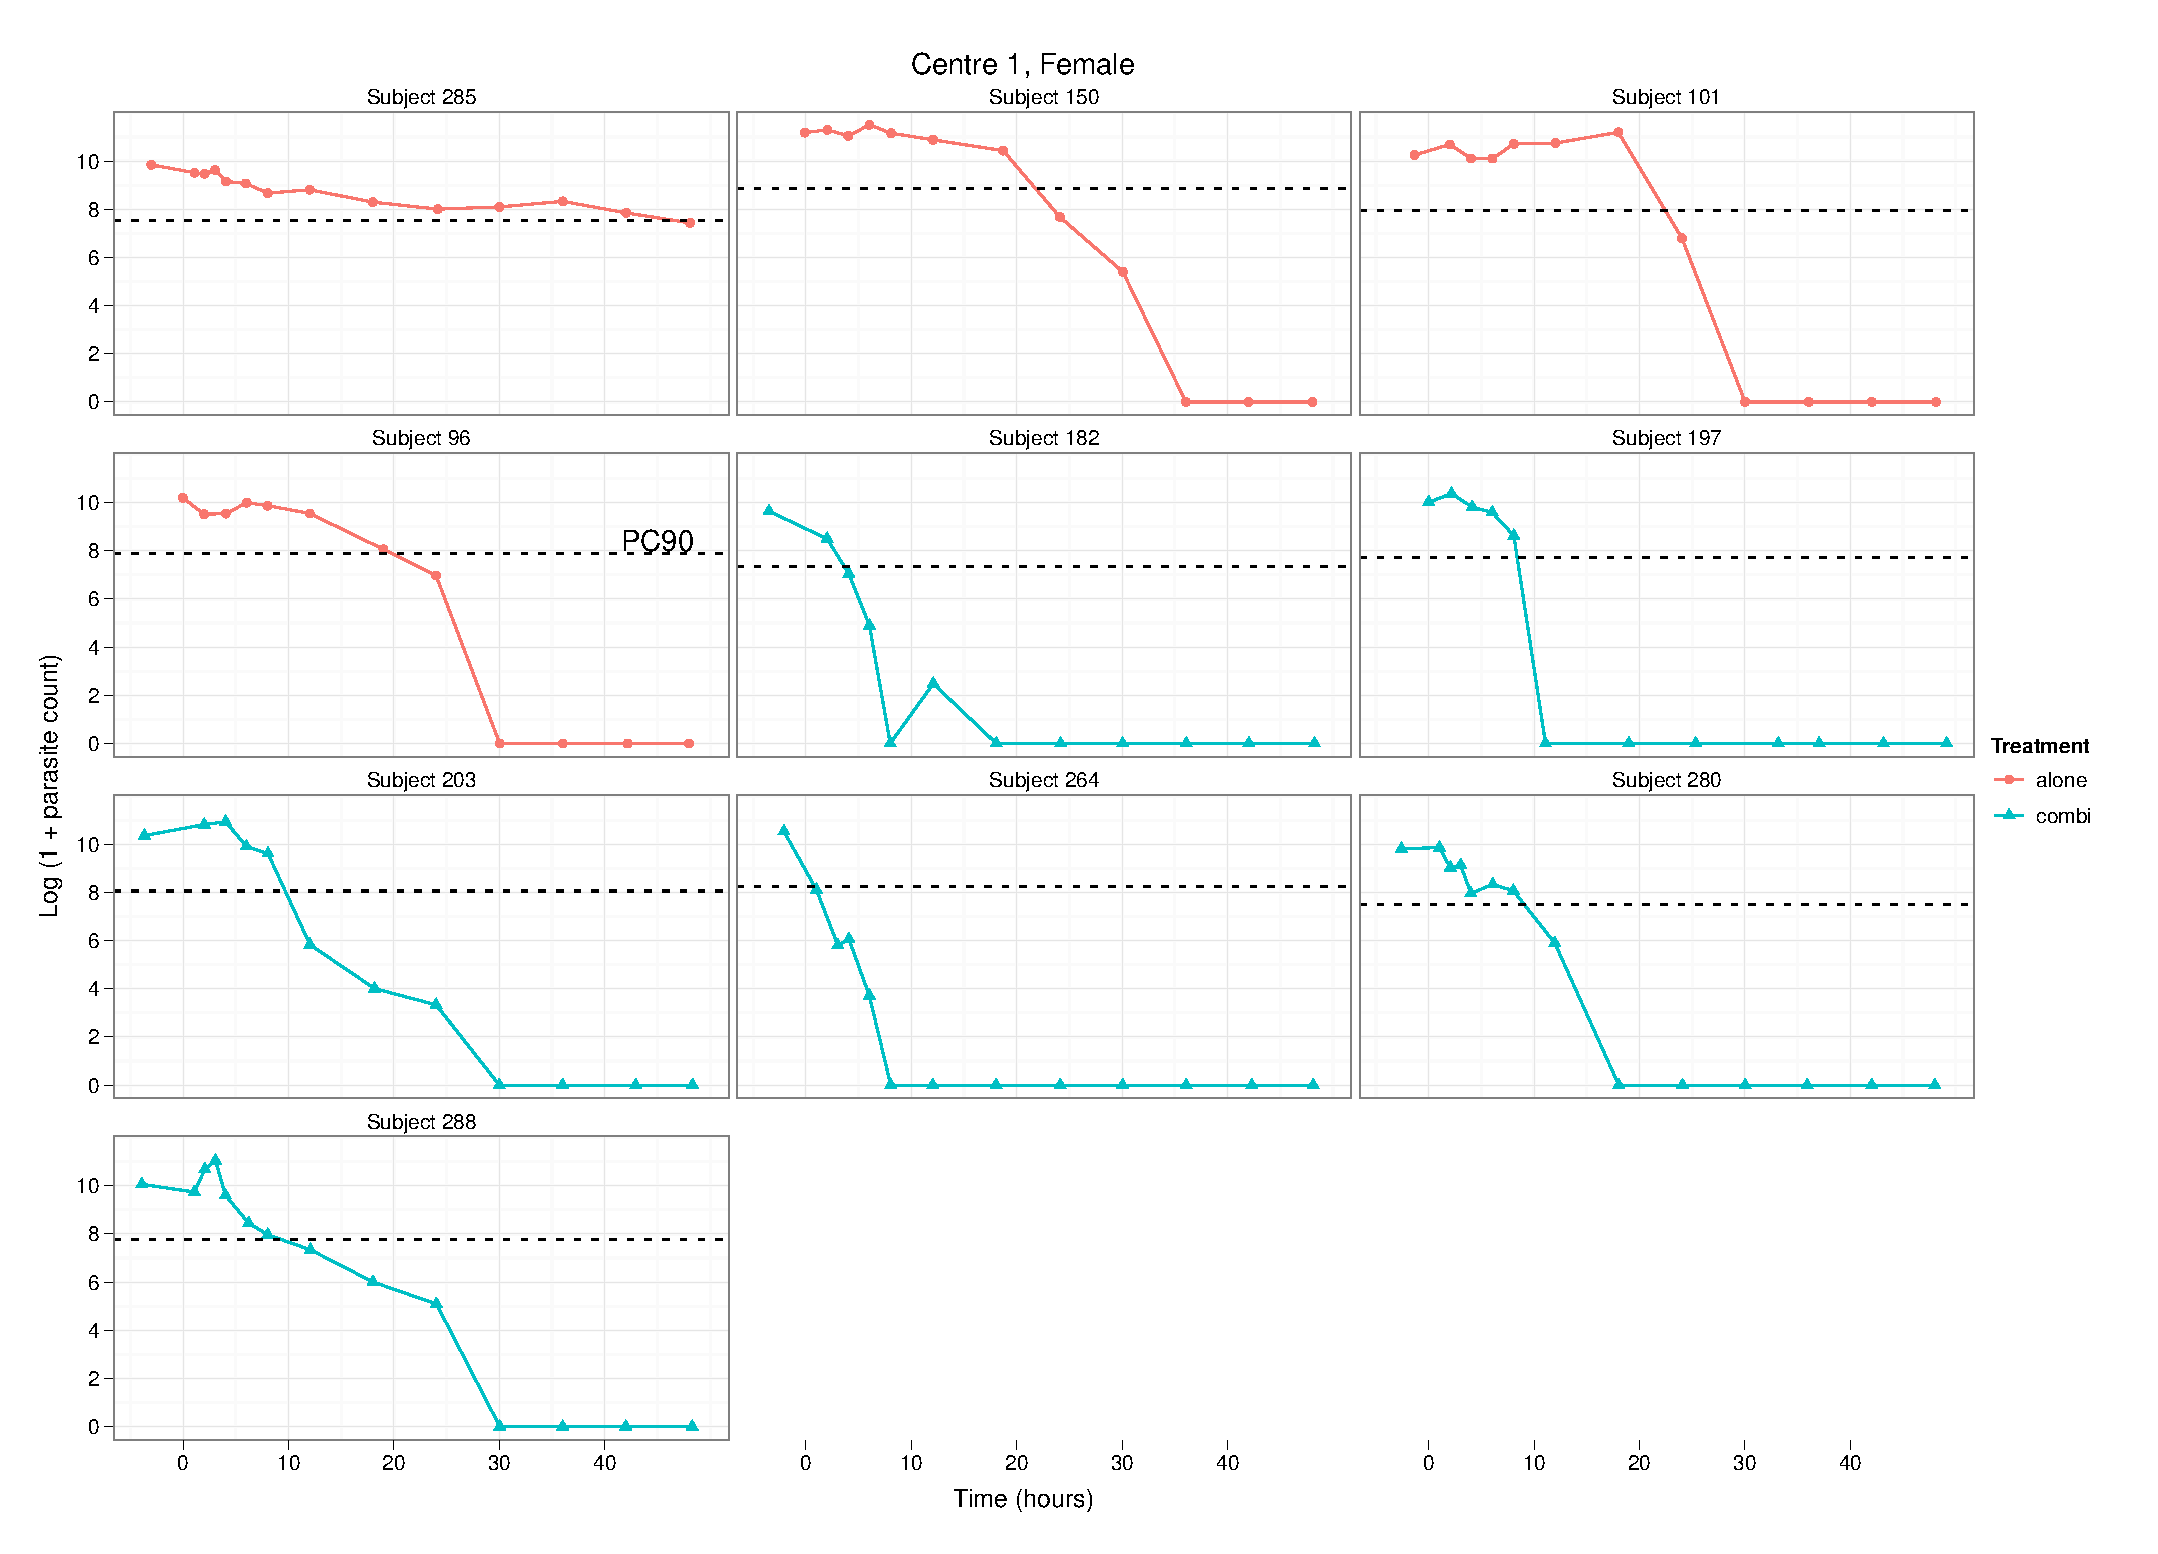
\includegraphics[height=150mm]{Araw1F.eps}
\end{sidewaysfigure}
\begin{sidewaysfigure}
\includegraphics[height=150mm]{Araw2M.eps}
\end{sidewaysfigure}
\begin{sidewaysfigure}
\includegraphics[height=150mm]{Araw2F.eps}
\end{sidewaysfigure}

\clearpage
\section{Model fits}
\begin{sidewaysfigure}
\includegraphics[height=150mm]{Afits1M.eps}
\end{sidewaysfigure}
\begin{sidewaysfigure}
\includegraphics[height=150mm]{Afits1F.eps}
\end{sidewaysfigure}
\begin{sidewaysfigure}
\includegraphics[height=150mm]{Afits2M.eps}
\end{sidewaysfigure}
\begin{sidewaysfigure}
\includegraphics[height=150mm]{Afits2F.eps}
\end{sidewaysfigure}

\chapter{\emph{R} code listings}
\lstset{numberstyle=\small,
frame=single,
framesep=6pt,
tabsize=2,
basicstyle=\small\ttfamily,
%keywordstyle=\bfseries,
%keywordstyle=\color{blue},
%commentstyle=\itshape\color{red},
showstringspaces=false,
columns = fullflexible,
language=R,
breaklines=true,
showstringspaces=false,
lineskip=-1pt}

\section{Functions for PC90 estimation}
\begin{lstlisting}[float=h,caption=Functions to find PC90 by cubic regression,label=R:cubics]
# Create a list of cubic fits to data up to first zero
cubic.fits <- function(data) {
	require(nlme)
	lmList(log(1 + parct) ~ acttm + I(acttm^2) + I(acttm^3) | SUBJID, data=uptofirstzero(data))
}

# Create a new data frame containing data up to first zero count
uptofirstzero <- function(data) {
	new.df <- data.frame()
	for (s in unique(data$SUBJID)) {
		rows <- data[data$SUBJID==s,]
		n <- match(0, rows$parct)
		if (!is.na(n)) {
			rows <- rows[1:n,]
		}
		new.df <- rbind(new.df, rows)
	}
	new.df
}

# Find the PC90 time from a cubic fit
pc90cubic <- function(fit, data) {
	coefs <- coef(fit)
	parct90 <- log(1 + (data$parct[data$plantm=='PRE-DOSE'] * 0.1))
	preds <- predict(fit)
	
	# Find the times at which counts are above and below PC90 
	upper <- which.min(preds > parct90)
	lower <- upper - 1
	interval <- c(data$acttm[lower], data$acttm[upper])

	# Search for PC90 between these times
	soln <- uniroot(function(x) coefs[1] + coefs[2]*x + coefs[3]*x^2 + coefs[4]*x^3 - parct90, interval=interval)
	soln$root
}
\end{lstlisting}

\begin{lstlisting}[float=h,caption=Functions to find PC90 by logistic regression,label=R:logistics]
# Perform logistic fitting after selecting starting parameters
logistic.fit <- function(dat) {
	# Set alpha and lambda to max and min counts
	initA <- max(log(1 + dat$parct))
	initL <- min(log(1 + dat$parct))

	# Set mu to time closest to half max count
	halfway <- (initA + initL)/2
	initU <- dat$acttm[which.min(abs(log(1 + dat$parct) - halfway))]

	# Set beta to -0.5 i.e. 2 in SSfpl formulation
	initB <- 2
	
	tryCatch(fit <- nls(log(1 + parct) ~ SSfpl(acttm, A, L, U, B), data=dat,
				start=list(A=initA, L=initL, U=initU, B=initB)),
		error=function(e) e)
	fit
}

# Find PC90 time from logistic fit
getPC90.logistic <- function(fit, data) {
	parct90 <- log(1 + (data$parct[data$plantm=='PRE-DOSE'] * 0.1))
	preds <- predict(fit)

	# Find the times at which counts are above and below PC90
	upper <- which.min(preds > parct90)
	lower <- upper - 1
	interval <- c(data$acttm[lower], data$acttm[upper])

	# Search for PC90 between these times
	soln <- uniroot(function(x) predict(fit, data.frame(acttm=x)) - parct90, interval=interval)
	soln$root
}
\end{lstlisting}

\begin{lstlisting}[float=h,caption=Functions to find PC90 by log-linear interpolation,label=R:loglinear]
# Get PCx time from log-linear interpolation
getPC.loglin <- function(data, PC=90) {
	pc <- log(1 + (data$parct[data$plantm=='PRE-DOSE'] * (100 - PC)/100))
	fit <- lmloglin(data, PC)
	B0 <- coef(fit)[1]
	B1 <- coef(fit)[2]
	(pc - B0) / B1
}

# Perform linear fit between two points either side of PCx
lmloglin <- function(data, PC=90) {
	lm(log(1 + parct) ~ acttm, data=data, subset=getAboveBelow(data, PC))
}

# Get indices of counts immediately above and below PCx level
getAboveBelow <- function(data, PC=90) {
	pc90 <- data$parct[data$plantm=='PRE-DOSE'] * (100 - PC)/100
	above.pc90 <- which(data$parct > pc90)
	upper <- above.pc90[length(above.pc90)]
	lower <- upper + 1
	c(upper, lower)
}
\end{lstlisting}

\clearpage
\section{Resampling functions}

\clearpage
\section{Functional data analysis}

\clearpage
\section{Plotting functions}
\begin{lstlisting}[float=h,caption=Plot raw count data for male and female subjects side-by-side,label=R:rawggplot]
# Plot raw data for male and female subjects side-by-side
rawggplot3 <- function(data, title="", centre="", r1=4, r2=4, points=T, lines=T) {
	require(ggplot2)

	vp1 <- viewport(width=0.45, x=0, just="left")
	q <- getrawplot(data[data$SEX=='Male',])
	q <- addtrtgeoms(q, points, lines)
	q <- q + opts(title=paste(centre, "Male"), legend.position='none')
	q <- q + facet_wrap(~SUBJID, nrow=r1, scales="free_y")
	print(q, vp=vp1)

	vp2 <- viewport(width=0.55, x=1, just="right")
	q <- getrawplot(data[data$SEX=='Female',])
	q <- addtrtgeoms(q, points, lines)
	q <- q + opts(title=paste(centre, "Female"))
	q <- q + facet_wrap(~SUBJID, nrow=r2, scales="free_y")
	print(q, vp=vp2)
}

# Set up the basic plot with data, scales and panels by subject
getrawplot <- function(data) {
	q <- ggplot(data, aes(x=acttm, y=parct))
	q <- q + scale_x_continuous(name="Time (hours)")
	q <- q + scale_y_continuous(formatter=function(x) return(x/1000), name="Parasite Count (1000s)")
	l <- length(unique(data$SUBJID))
	q + facet_wrap(~SUBJID, ncol=min(3,l), scales="free_y")
}

# Change point shape and line colour to reflect treatment group
addtrtgeoms <- function(q, points=T, lines=T) {
	# Reorder the patient factor so that "alone" treatment patients are first
	for(subj in as.character(unique(q$data$SUBJID[q$data$trt=='A']))) {
		q$data$SUBJID <- relevel(q$data$SUBJID, subj)
	}
	if (points) {
		q <- q + geom_point(aes(shape=trttxt, colour=trttxt))
	}
	if (lines) {
		q <- q + geom_line(aes(colour=trttxt))
	}
	q + scale_shape(name="Treatment") + scale_colour_discrete("Treatment")
}
\end{lstlisting}

\begin{lstlisting}[float=h,caption=Boxplots of pre-dose count by sex\, centre and treatment,label=R:predoseaov]
# Plot pre-dose counts as boxplots by centre, sex and treatment
predoseaov2 <- function(data) {
	require(ggplot2)

	# Boxplots of pre-dose count by sex for each centre
	vp1 <- viewport(width=1, height=0.33, y=1, just="top")
	q1 <- qplot(SEX, parct, data=data, geom="blank", colour=SEX, xlab="Sex:Centre", ylab="")
	q1 <- q1 + scale_colour_discrete(h.start=120)
	q1 <- q1 + scale_y_continuous(limits=c(0,100000), formatter="comma")
	q1 <- q1 + geom_boxplot(width=0.3, outlier.size=0)
	q1 <- q1 + geom_point(position=position_jitter(w=0.1))
	q1 <- q1 + opts(legend.position="none")
	q1 <- q1 + facet_grid(.~CENTREID)
	print(q1, vp=vp1)

	# Boxplots of pre-dose count by treatment for each centre
	vp2 <- viewport(width=1, height=0.33, y=0.5, just="centre")
	q2 <- qplot(trttxt, parct, data=data, geom="blank", colour=trttxt, xlab="Treatment:Centre", ylab="Parasite Count")
	q2 <- q2 + scale_y_continuous(limits=c(0,100000), formatter="comma")
	q2 <- q2 + geom_boxplot(width=0.3, outlier.size=0)
	q2 <- q2 + geom_point(position=position_jitter(w=0.1))
	q2 <- q2 + opts(legend.position="none")
	q2 <- q2 + facet_grid(.~CENTREID)
	print(q2, vp=vp2)

	# Boxplots of pre-dose count by treatment for each sex
	vp3 <- viewport(width=1, height=0.33, y=0, just="bottom")
	q3 <- qplot(trttxt, parct, data=data, geom="blank", colour=trttxt, xlab="Treatment:Sex", ylab="")
	q3 <- q3 + scale_y_continuous(limits=c(0,100000), formatter="comma")
	q3 <- q3 + geom_boxplot(width=0.3, outlier.size=0)
	q3 <- q3 + geom_point(position=position_jitter(w=0.1))
	q3 <- q3 + opts(legend.position="none")
	q3 <- q3 + facet_grid(.~SEX)
	print(q3, vp=vp3)
}
\end{lstlisting}

\begin{lstlisting}[float=h,caption=Residuals diagnostic plots for \texttt{lm,aov} fitted models,label=R:plotresids.lm]
# Residuals diagnostics plots for lm/aov fit
plotresids.lm <- function(model, resids, data, binwidth=0.5, trans=F, weighted=F, xlab="Fitted PC90 (hours)") {
	require(ggplot2)
	require(MASS)
	if (missing(resids)) {
		resids <- stdres(model)
	}
	if (missing(data)) {
		data <- model$model
	}
	lab.txt <- "Standardized residuals"

	# Histogram
	vp1 <- viewport(width=0.5, height=0.5, x=0.25, y=0.75)
	q <- qplot(resids, xlab=lab.txt, geom="blank") + geom_histogram(colour="black", fill="white", binwidth=binwidth) 
	print(q, vp=vp1)

	# QQ normal
	vp2 <- viewport(width=0.5, height=0.5, x=0.75, y=0.75)
	q <- qplot(sample=resids)
	y <- quantile(resids, c(0.25, 0.75))
	x <- qnorm(c(0.25, 0.75))
	slope <- diff(y)/diff(x)
	int <- y[1L] - slope * x[1L]
	q <- q + geom_abline(intercept=int, slope=slope, linetype=2)
	print(q, vp=vp2)

	# vs factors
	vp3 <- viewport(width=0.5, height=0.5, x=0.25, y=0.25)
	p <- dim(data)[2] - weighted
	data.l <- reshape(data, direction="long", varying=list(2:p), v.names="Factor")
	if (p > 2)
		q <- qplot(Factor, rep(resids, p-1), data=data.l, geom="blank", ylab=lab.txt, colour=time)
	else
		q <- qplot(Factor, resids, data=data.l, geom="blank", ylab=lab.txt)
	q <- q + geom_hline(aes(yintercept=0), linetype=2)
	q <- q + geom_point(position=position_jitter(w=0.1))
	if (is.factor(data$Factor))
		q <- q + stat_summary(fun.dat="mean_sdl", mult=1, geom="crossbar", width=0.5)
	q <- q + opts(legend.position="none")
	print(q, vp=vp3)

	# vs fitted
	vp4 <- viewport(width=0.5, height=0.5, x=0.75, y=0.25)
	q <- qplot(fitted(model)^(1+1*trans), resids, data=data, xlab=xlab, ylab=lab.txt)
	q <- q + geom_hline(aes(yintercept=0), linetype=2)
	print(q, vp=vp4)
}
\end{lstlisting}

\begin{lstlisting}[float=h,caption=Plot all 3 PC90 methods on same plot,label=R:comparePC90]
# All 3 PC90 estimation methods on same plot
comparePC90 <- function(dat, pc90, logfit=T, ...) {
	q <- getrawplot(dat) + geom_point(shape=1)
	q <- getlogplot(q)
	q <- addPC90lines(q, logplot=T)
	q <- addcubicfit(q, colour="blue")
	if (logfit) {
		tryCatch(q <- addlogfit(q, colour="red", ...), error=function(e) {})
	}
	q <- addloglin(q, colour="green")
	addPC90vlines(q, pc90) + facet_wrap(~SUBJID, ncol=2)
}

# Convert the plot q to log-linear
getlogplot <- function(q) {
	q <- q %+% transform(q$data, parct=log(1+parct))
	q <- q + scale_y_continuous(name="Log (1 + parasite count)")
	l <- length(unique(q$data$SUBJID))
	q + facet_wrap(~SUBJID, ncol=min(3,l), scales="fixed")
}

# Add cubic fit to plot q
addcubicfit <- function(q, ...) {
	q + stat_smooth(method="lm", formula=y~x+I(x^2)+I(x^3), data=uptofirstzero(q$data), fullrange=F, se=F, ...) 
}

# Add logistic fit to plot q
addlogfit <- function(q, ...) {
	q + stat_smooth(method="nls", formula="y ~ SSfpl(x, A, L, U, B)", se=F, ...)
}

# Add log-linear interpolation to plot q
addloglin <- function(q, ...) {
	dat <- q$data
	dat$parct <- exp(q$dat$parct) - 1
	dat <- by(dat, dat$SUBJID, getAboveBelow)
	data <- data.frame()
	for (s in unique(q$data$SUBJID)) {
		data <- rbind(data, q$data[q$data$SUBJID==s,][dat[[s]],])
	}
	q + geom_line(data=data, ...)
}

# Add vertical lines showing 3 PC90 estimates
addPC90vlines <- function(q, dat, colours=c("blue", "red", "green")) {
	dat <- subset(dat, subset=SUBJID %in% unique(q$data$SUBJID))
	q + geom_vline(data=dat, aes(xintercept=PC90, colour=method), linetype=2) + scale_colour_manual(values=colours)
}
\end{lstlisting}

\begin{lstlisting}[float=h,language=SAS,caption=SAS,label=SAS]
data subjects;
	set Project.Msc_data;
	x=acttm;
	y=log(1+parct);
	run;
data predose;
	set Project.Msc_data (keep=SUBJID plantm parct);
	if plantm eq 'PRE-DOSE';
	l90 = log(1 + (0.1 * parct));
	run;	
proc nlin data=subjects;
	parms A=0 to 12 L=8 to 14 B=-0.5 to 0 by 0.1  U=5 to 20 by 5;
	model y=A+(L/(1+exp(-B*(x-U))));
	by SUBJID;
	output out=nlinfit p=pred;
	run;
quit;
data plotdata;
	merge nlinfit predose;
	by SUBJID;
	run;
symbol1 c=black i=none v=x;
symbol2 c=blue i=join v=none;
symbol3 c=black i=join l=2 v=none;
proc gplot data=plotdata;
	plot (y pred l90)*x / overlay;
	by SUBJID;
	run;
quit;
\end{lstlisting}
\end{document}